\PassOptionsToPackage{dvipsnames}{xcolor}
\documentclass[UTF8,12pt]{ctexart}

% 显式给 Fandol 中文字体登记 small-caps 形状。
% 模板的 \ChapterSectionLabel 与 titlepage 都用到 \textsc / \scshape，
% 默认查不到 CJK 字体的 sc 形状会出现 "Font shape ... sc undefined" 警告；
% 这里把 sc 显式落到 Regular/Hei，警告消失，输出无可见变化（中文本无大小写之分）。
\setCJKmainfont{FandolSong-Regular}[
  Extension  = .otf,
  ItalicFont = FandolKai-Regular,
  BoldItalicFont = FandolKai-Regular,
  Script = Default,
  BoldFont   = FandolHei-Regular,
  FontFace   = {m}{sc}{Font=FandolSong-Regular},
  FontFace   = {bx}{sc}{Font=FandolHei-Regular},
]

\usepackage[paper=a4paper,left=2.5cm,right=2.5cm,top=3cm,bottom=3cm]{geometry}
\usepackage{amsmath,amsthm,amssymb,mathrsfs,bbm,needspace}
\usepackage{graphicx,tikz-cd,titlesec}
\usepackage[dvipsnames]{xcolor}
\usepackage[
    colorlinks=true,
    linkcolor=MidnightBlue,
    citecolor=BrickRed,
    urlcolor=MidnightBlue,
    linktoc=all
]{hyperref}

\pagestyle{plain}

% 设置环境
\usepackage{aliascnt}
\theoremstyle{plain}
\newtheorem{theorem}{定理}[section]
\newaliascnt{definition}{theorem}
\newtheorem{definition}[definition]{定义}
\aliascntresetthe{definition}
\newaliascnt{lemma}{theorem}
\newtheorem{lemma}[lemma]{引理}
\aliascntresetthe{lemma}
\newaliascnt{corollary}{theorem}
\newtheorem{corollary}[corollary]{推论}
\aliascntresetthe{corollary}
\newaliascnt{remark}{theorem}
\newtheorem{remark}[remark]{注}
\aliascntresetthe{remark}
\newaliascnt{example}{theorem}
\newtheorem{example}[example]{例}
\aliascntresetthe{example}
\newaliascnt{proposition}{theorem}
\newtheorem{proposition}[proposition]{命题}
\aliascntresetthe{proposition}
\newaliascnt{problem}{theorem}
\newtheorem{problem}[problem]{问题}
\aliascntresetthe{problem}
\newtheorem{exercise}{习题}
\numberwithin{equation}{section}
\numberwithin{figure}{section}

% autoref names
\providecommand{\sectionautorefname}{章}
\renewcommand{\sectionautorefname}{章}

\providecommand{\subsectionautorefname}{节}
\renewcommand{\subsectionautorefname}{节}

\providecommand{\definitionautorefname}{定义}
\renewcommand{\definitionautorefname}{定义}

\providecommand{\theoremautorefname}{定理}
\renewcommand{\theoremautorefname}{定理}

\providecommand{\lemmaautorefname}{引理}
\renewcommand{\lemmaautorefname}{引理}

\providecommand{\propositionautorefname}{命题}
\renewcommand{\propositionautorefname}{命题}

\providecommand{\corollaryautorefname}{推论}
\renewcommand{\corollaryautorefname}{推论}

\providecommand{\exampleautorefname}{例}
\renewcommand{\exampleautorefname}{例}

\providecommand{\remarkautorefname}{注}
\renewcommand{\remarkautorefname}{注}

\providecommand{\exerciseautorefname}{习题}
\renewcommand{\exerciseautorefname}{习题}

\providecommand{\problemautorefname}{问题}
\renewcommand{\problemautorefname}{问题}

\providecommand{\figureautorefname}{图}
\renewcommand{\figureautorefname}{图}

\providecommand{\tableautorefname}{表}
\renewcommand{\tableautorefname}{表}

% 设置 proof 样式
\makeatletter
\renewcommand{\proofname}{\textbf{证明}}
\renewenvironment{proof}[1][\proofname]{\par
  \pushQED{\qed}%
  \normalfont
  \topsep6\p@\@plus6\p@\relax
  \trivlist
  \item[\hskip\labelsep
        \normalfont\bfseries
    #1\@addpunct{.}]\ignorespaces
}{%
  \popQED\endtrivlist\@endpefalse
}
\makeatother
\renewcommand{\qedsymbol}{\ensuremath{\square}}

% 设置 section 样式
\newlength{\chapterNumSpace}
\setlength{\chapterNumSpace}{1.4cm}

% 附录判断：正文显示 Chapter，\appendix 后显示 Appendix
\newif\ifInAppendix
\InAppendixfalse

% 目录中的附录判断
\newif\ifInAppendixToc
\InAppendixTocfalse

% 目录可调参数
\newlength{\tocSectionLabelWidth}
\setlength{\tocSectionLabelWidth}{4.2em}

\newlength{\tocAppendixGap}
\setlength{\tocAppendixGap}{0.2em}

\newlength{\tocSubIndent}
\setlength{\tocSubIndent}{1.2em}

\newlength{\tocSubNumWidth}
\setlength{\tocSubNumWidth}{3.0em}

% 目录 section 编号文字
\newcommand{\TocSectionNumber}[1]{%
  \ifInAppendixToc
    附录\hspace{\tocAppendixGap}#1%
  \else
    第~#1~章%
  \fi
}

\makeatletter

% section 目录格式：
% 正文：第 1 章 群的定义与性质
% 附录：附录A 集合论补遗
\renewcommand*\l@section[2]{%
  \ifnum\c@tocdepth>\z@
    \addvspace{0.55em}%
    \begingroup
      \parindent\z@
      \rightskip\@pnumwidth
      \parfillskip-\@pnumwidth
      \leavevmode
      \bfseries
      \setlength{\@tempdima}{\tocSectionLabelWidth}%
      \advance\leftskip\@tempdima
      \hskip-\leftskip
      \def\numberline##1{%
        \makebox[\@tempdima][l]{\TocSectionNumber{##1}}%
      }%
      #1\nobreak\hfill\nobreak\makebox[\@pnumwidth][r]{#2}\par
    \endgroup
  \fi
}

% subsection 目录格式：
% 1.1 循环群 / A.1 集合基础
\renewcommand*\l@subsection{%
  \@dottedtocline{2}{\tocSubIndent}{\tocSubNumWidth}%
}

\makeatother

\let\OriginalAppendix\appendix
\renewcommand{\appendix}{%
  \OriginalAppendix
  \InAppendixtrue
  \addtocontents{toc}{\protect\InAppendixToctrue}%
}

\newcommand{\ChapterSectionLabel}{%
  \thispagestyle{plain}%
  \vspace*{-0.5cm}%
  \makebox[\textwidth][r]{%
    {\fontsize{18pt}{18pt}\selectfont\scshape
      \ifInAppendix 附录\else 第\fi
    }\enspace
    {\fontsize{62pt}{62pt}\selectfont\bfseries\thesection}\enspace{\fontsize{18pt}{18pt}\selectfont\ifInAppendix\else 章\fi}%
  }%
  \par\vspace{-0.25cm}%
  \noindent\rule{\dimexpr\textwidth-\chapterNumSpace\relax}{0.45pt}%
}

\titleformat{\section}[display]
  {\normalfont}
  {\ChapterSectionLabel}
  {0cm}
  {\raggedleft\rightskip=\chapterNumSpace\fontsize{30pt}{35pt}\selectfont\bfseries}
  [\vspace{0.3cm}]

\newcommand{\sectionbreak}{\clearpage}

% 不编号 section，例如前言、目录
\titleformat{name=\section,numberless}[block]
  {\normalfont\Large\bfseries\centering}
  {}
  {0pt}
  {}

% section 整体间距
\titlespacing{\section}
  {0pt}
  {0pt}
  {0pt}

% subsection 样式
\ctexset{
  subsection = {
    format = \large\bfseries
  }
}



\usepackage[most]{tcolorbox}
\usepackage{xurl,longtable}
% 仅登记平均积分符号，保留模板原有积分字体.
\DeclareSymbolFont{sourceaveragesymbols}{U}{esint}{m}{n}
\DeclareMathSymbol{\fintop}{\mathop}{sourceaveragesymbols}{'037}
\newcommand{\fint}{\fintop\nolimits}
\newfontfamily\SourceAccentFont{Times New Roman}
\newtheoremstyle{boxedsource}{0pt}{0pt}{\normalfont}{}{\bfseries}{.}{.5em}{}
\theoremstyle{boxedsource}
\newtheorem*{definition*}{定义}
\newtheorem*{example*}{例}
\newtheorem*{proposition*}{命题}
\newtheorem*{theorem*}{定理}
\newtheorem*{problem*}{问题}
\newtheorem*{openproblem}{未解问题}
\theoremstyle{plain}
\setlength{\emergencystretch}{1em}
\newcounter{boxcounter}[section]
\renewcommand{\theboxcounter}{\thesection.\arabic{boxcounter}}
\providecommand{\boxcounterautorefname}{知识框}
\newenvironment{sourcebox}[1]{\refstepcounter{boxcounter}\begin{tcolorbox}[breakable,colback=gray!4,colframe=gray!55,title={知识框~\theboxcounter\quad #1},fonttitle=\bfseries,coltitle=black]}{\end{tcolorbox}}
\newcommand{\orig}[2]{\href[page=#1]{../../books/Santambrogio 2015 Optiomal Transport For Applied Mathematicians.pdf}{#2}}
\providecommand{\subsubsectionautorefname}{节}
\renewcommand{\subsubsectionautorefname}{节}
\renewcommand{\refname}{参考文献}
\hypersetup{pdftitle={应用数学家的最优运输：前置内容与第1章中文译稿},pdfauthor={Filippo Santambrogio},bookmarksnumbered=true}
\newcommand{\id}{\operatorname{id}}
\newcommand{\spt}{\operatorname{spt}}
\newcommand{\Lip}{\operatorname{Lip}}
\newcommand{\Per}{\operatorname{Per}}
\newcommand{\cof}{\operatorname{cof}}
\newcommand{\Tr}{\operatorname{Tr}}
\newcommand{\R}{\mathbb R}
\newcommand{\N}{\mathbb N}
\newcommand{\dd}{\,\mathrm d}
\newcommand{\restr}{\mathbin{\vrule height 1.4ex depth -.1ex width .07ex\vrule height .07ex depth -.0ex width .7ex}}
\begin{document}
\hypersetup{pageanchor=false}
% 原件物理1、4；沿用本库已用中文模板，不复刻封面装饰.
\begin{titlepage}
\flushleft
\rule{\textwidth}{1.2pt}\\[.1cm]\rule{\textwidth}{.8pt}\\[1.4cm]
{\fontsize{36pt}{48pt}\selectfont\bfseries 应用数学家的\\最优运输}\\[.8cm]
{\Large\itshape Optimal Transport for Applied Mathematicians}\\[.8cm]
\rule{\textwidth}{.6pt}\\[.8cm]
{\Large 变分法、偏微分方程与建模}\\[.3cm]
{\large Calculus of Variations, PDEs, and Modeling}\\[1cm]
{\Large Filippo Santambrogio}\\[1cm]
{\small Progress in Nonlinear Differential Equations and Their Applications 87\\Birkhäuser / Springer，2015}
\vfill
{\small 中文全译稿\\2026年11月4日\\原书作者、编号与论证次序保留；具体核验范围见随附说明.}
\end{titlepage}

\pagenumbering{roman}\hypersetup{pageanchor=true}
% 原件物理3、5、6；原文人名和机构名保留以便溯源.
\section*{丛书信息}\phantomsection\addcontentsline{toc}{section}{丛书信息}
\begin{center}\large 非线性偏微分方程进展及其应用\\Progress in Nonlinear Differential Equations and Their Applications\\第87卷\end{center}
\noindent\textbf{主编}\\Haim Brezis\\Université Pierre et Marie Curie，法国巴黎\\以及 Rutgers University，美国新泽西州新不伦瑞克.

\noindent\textbf{编委会}
\begin{small}\begin{itemize}
\item Antonio Ambrosetti，Scuola Internationale Superiore di Studi Avanzati，意大利的里雅斯特.
\item A. Bahri，Rutgers University，美国新泽西州新不伦瑞克.
\item Felix Browder，Rutgers University，美国新泽西州新不伦瑞克.
\item Luis Caffarelli，The University of Texas，Austin，美国得克萨斯州.
\item Lawrence C. Evans，University of California，Berkeley，美国加利福尼亚州.
\item Mariano Giaquinta，University of Pisa，意大利比萨.
\item David Kinderlehrer，Carnegie-Mellon University，美国宾夕法尼亚州匹兹堡.
\item Sergiu Klainerman，Princeton University，美国新泽西州普林斯顿.
\item Robert Kohn，New York University，美国纽约州纽约.
\item P. L. Lions，University of Paris IX，法国巴黎.
\item Jean Mawhin，Université Catholique de Louvain，比利时新鲁汶.
\item Louis Nirenberg，New York University，美国纽约州纽约.
\item Lambertus Peletier，University of Leiden，荷兰莱顿.
\item Paul Rabinowitz，University of Wisconsin，美国威斯康星州麦迪逊.
\item John Toland，University of Bath，英国巴斯.
\end{itemize}\end{small}
丛书详情：\url{http://www.springer.com/series/4889}.
\clearpage
\section*{题名与版权}\phantomsection\addcontentsline{toc}{section}{题名与版权}
\noindent Filippo Santambrogio\\Laboratoire de Mathématiques d'Orsay\\Université Paris-Sud\\法国奥赛.
\vspace{1em}

\noindent ISSN 1421-1750；电子ISSN 2374-0280.\\
纸本ISBN 978-3-319-20827-5；电子书ISBN 978-3-319-20828-2.\\
DOI：\href{https://doi.org/10.1007/978-3-319-20828-2}{\nolinkurl{10.1007/978-3-319-20828-2}}.\\
美国国会图书馆控制号：2015946595.

\noindent 2010年数学主题分类：49J45，90C05，35J96，35K10，39B62，90B06，91A13，90B20，26B25，49N15，52A41，49M29，76M25.

\noindent Springer：Cham、Heidelberg、New York、Dordrecht、London.\\
\copyright\ Springer International Publishing Switzerland 2015.

本作品受版权保护. 全部权利由出版者保留，无论涉及全部还是部分材料，包括翻译、重印、插图再利用、朗诵、广播、缩微胶片或其他物理形式的复制，以及信息传输、存储与检索、电子改编、计算机软件，或以现已知晓或今后开发的类似或不同方式进行的使用.

本出版物使用通用描述性名称、注册名称、商标、服务标志等，即使没有特别声明，也不意味着这些名称不受有关保护法律法规约束，或可以自由地为一般用途使用.

出版者、作者和编者认为，本书中的建议与信息在出版时真实而准确. 对于书中所载材料，以及可能存在的错误或遗漏，出版者、作者和编者均不作明示或默示的保证.

本书采用无酸纸印刷.

Springer International Publishing AG Switzerland 隶属于 Springer Science+Business Media（\href{https://www.springer.com}{\nolinkurl{www.springer.com}}）.
\clearpage
\thispagestyle{plain}\vspace*{.25\textheight}
\begin{flushright}\itshape
献给我亲爱的妻子Anna.\\
她很生气，因为我的书\\
比她的书构思得晚，却早得多就完成了\ldots\\
不过，她似乎依然爱我.
\end{flushright}\clearpage

% 原文前言：印刷vii–xiii／PDF物理8–14.
\section*{前言}\phantomsection\label{sec:preface}\addcontentsline{toc}{section}{前言}
\subsection*{为什么写这本书？}
为什么还要写一本最优运输（optimal transport）的书？菲尔兹奖得主Cédric Villani的两本书还不够吗？还有Luigi Ambrosio、Nicola Gigli和Giuseppe Savaré撰写的梯度流“圣经”，其中同样包含许多关于最优运输的高级而一般的细节.

本书很松散地受到我2011、2012年在奥赛开设的课程，以及更早在格勒诺布尔暑期学校讲授的两门短期入门课程\cite{b274,b275}的启发，希望提出不同的视角，也部分面向不同的读者群体. 目前，将最优运输作为工具从事应用数学研究的群体正在不断扩大. 例如图像处理、经济学和演化偏微分方程，后者尤其涉及生物学或社会科学中的群体动力学建模，以及流体力学. 更一般地，在应用数学中，最优运输既是进行证明、估计和设计数值方法的技术工具，也是描述涉及距离、路径和成本的现象的建模工具.

从这一侧进入最优运输的读者最关心的问题包括：怎样数值计算最优映射与成本；问题有哪些不同表述，以便将其用于新的模型和目的；怎样以尽可能具体的方式得到连接运输与偏微分方程的主要结果；以及怎样运用该理论研究已有模型. 我们不能说已有著作没有回答这些问题，但很可能没有一本是以此为写作目的的.

C. Villani的第一本书\cite{b292}最接近我们的意图. 它广泛介绍这一主题及其应用，适合各种读者. 但我决定在这里讨论的一些主题并未在\cite{b292}中描述，例如本书\hyperref[sec:4]{第4章}的最小流问题. 而且，自2003年以来，这一理论已经取得巨大进展. ST Rachev和L Ruschednorf的两卷著作\cite{b257,b258}也不应被忘记，其中涉及许多概率与统计应用. 不过，它们的研究范围很快便与本书分开，因此我们不会展开\cite{b257}中的大部分应用和语言. 我们主要坚持确定性的框架与变分法的风格.

如果考察\cite{b292}之后的发展，至少应提到此后出版的两部优美著作. C. Villani的新书\cite{b293}将原先的介绍扩充为近千页的篇幅，增加的内容大多涉及几何问题，尤其是曲率概念. 流形上二次成本的最优运输成为核心工具，也是研究度量测度空间的出发点. 另一部参考书是L. Ambrosio、N. Gigli和G. Savaré的著作\cite{b15}，研究度量空间，尤其是概率测度的Wasserstein空间中的梯度流演化. 这一主题有许多有趣应用，例如热方程、Fokker--Planck方程与多孔介质方程，所发展的工具也非常有用. 但作者的主要视角是研究这些抽象空间中隐藏的微分结构；建模与应用数学大概并非他们首先关注的事情.

上述部分文献技术性很强，发展了能够适用于非常一般情形的强大抽象工具，但许多读者可能难以使用. 因而后来出现了一些较短的综述和更容易处理的讲义，例如\cite{b11}对\cite{b15}部分内容的简化，以及L. Ambrosio和N. Gigli撰写的简短入门\cite{b9}. 然而，仔细分析\cite{b9}便会发现，前半部分介绍带有某些变化的最优运输一般理论，余下部分讨论一般度量空间的梯度流，以及具有曲率下界的度量测度空间. 还应提到两篇很新的综述\cite{b63,b228}：前者在L. V. Kantorovich诞辰百年之际回顾该理论的主要成果，后者则对这一主题及其与几何和经济学的联系作总体介绍.

与此同时，许多活动凸显了人们对最优运输应用侧面日益增长的兴趣：出版物\footnote{ESAIM M2AN的“Optimal Transport in Applied Mathematics”专刊正在筹备；本书部分参考文献取自该专刊.}、学校、研讨会、研究项目等. 自2010年代以来，这个群体十分活跃，尤其在法国，也包括加拿大、意大利、奥地利、英国等地. 这些考虑使我觉得，撰写一本专门的书可能是个好主意；你现在手中的这本书，就是过去三年工作的成果.

\subsection*{这本书有什么特点？}
本书严格介绍最优运输理论及一些受到忽视的变体，并解释它与演化偏微分方程、图像处理和经济学中许多主题之间最重要的联系.

我尽可能避开最一般的框架，将注意力集中于欧氏情形；但若在Polish空间中陈述结果并不增加困难，反而有助于澄清图景，也会采用这一表述. 只要加上紧性假设能够简化叙述，又不至于过多降低结论的意义——当然是依照我的个人判断——我便借此略过一些困难. 许多时候，我也先从最简单的情形，例如具有紧性或连续性的情形讲起，然后再推广.

在可以选择时，我尽量采用更“具体”的证明，因为我认为读者更容易理解. 例如，Wasserstein空间中Lipschitz曲线的速度场存在性，在这里通过逼近证明；而\cite{b15}采用抽象泛函分析工具，关键是巧妙运用Hahn--Banach定理.

我没有试图穷尽所有可能的主题，而是把全书分为八章，大致各对应一讲较长的课程. 显然，我增加了许多通常一讲之内无法涉及的材料，但主题的选择与顺序确实遵循2011年奥赛的一门八讲课程；仅有的例外是\autoref{sec:1}与\hyperref[sec:5]{第5章}各用了约一讲半，后续章节在2011年则缩短为半讲. 距离这八“讲”的主题太远的内容，不放入各章主体. 另一方面，每章末尾都有讨论部分，介绍推广、联系、旁支主题及不同观点. 在某些情形，例如拥挤运输与分支运输，这些讨论部分相当于相关运输模型的小型综述. 其风格较为非正式：有时证明陈述，有时只给出草图或提及结果.

为了扩大读者群，让尽可能多的人能够阅读，我决定详细解释一些原本可以假定读者已知的记号——不过，回顾它们总是更好. 各章通过称为“回顾”（Memo）或“重要概念”（Important Notion）的专门知识框回顾部分概念\footnote{两者的区别只是：在后一种情形，我本来更愿意将其视为“回顾”，但学生通常不同意.}. 第三种知识框称为“值得了解”（Good to Know!），提供通常不属于非专门方向数学研究生背景知识的额外概念. 随着全书推进，知识框和说明图的密度都会降低.

为求简便，我决定不反复强调至少一个重要问题：可测性. 你可以相信，书中引入的集合、函数和映射都具有所需的可测性，但我不会逐一明确说明. 实际上，这是我对不够严密所作的唯一让步：全书证明是严格的，至少我希望如此，纯数学家或应用数学家都可以将其作为有关主题的参考. 唯一叙述略显非正式的是关于数值方法的\hyperref[sec:6]{第6章}，这里的意思是我们不提供收敛证明或精确的实现细节.

最后但并非最不重要的是：本书有一章数值方法！尤其介绍与偏微分方程联系最紧密的连续方法，而组合性和离散性最强的方法则在讨论部分简述.

\subsection*{这本书写给谁？}
本书采用应用数学家的视角，应用数学家理应是其自然读者. 不过，我希望与更广泛的读者交流. 纯数学家当然也受到欢迎——纯数学与应用数学之间的区别是否有意义，本来就是个人判断. 他们会看到严格的证明，有时受到不同视角的启发；也可能有兴趣发现最优运输能够用在何处、怎样使用，并作出自己的贡献.

更一般地，可以把区分移到“使用最优运输工作的人”和“研究最优运输本身的人”之间. 前者是本书的自然读者，但后者也可能对内容感兴趣. 反过来，本书是否也面向非数学家，例如物理学家、工程师和理论经济学家？这涉及读者需要多少数学背景. 显然，如果他们有足够的数学背景，而且工作领域与书中应用足够接近，了解这些应用背后的内容会很有意思.

需要多少数学也同样是学生面对的问题. 这是一本数学研究生教材. 即使我试图提供工具，帮助回顾所需背景，要充分利用本书，仍然需要一定先修知识. 主要先修内容是测度论与泛函分析. 我特意没有采纳某位“匿名”审稿人关于加入测度论附录的建议. 我的想法是，希望接近最优运输的数学工作者，应当已经对这些主题有所了解：什么是可测函数、什么是测度、主要收敛定理的条件是什么，以及$L^p$与$W^{1,p}$函数、弱收敛等. 回顾框的作用是帮助读者不至于迷失. 对于阅读本书的非数学家，我希望更具体的处理方式能帮助他们看出哪些性质重要而合理；但这些读者也应掌握一些数学语言，而且肯定需要付出额外努力，才能充分受益.

关于读者，数值部分，即\hyperref[sec:6]{第6章}，还值得多说几句. 详细比较各种方法的优缺点、讨论实现中最巧妙的技巧，以及最新算法，都超出本书范围. 因而，已经研究这一领域的人大概用不上这一章. 另一方面，使用最优运输但不了解数值方法的人，或尚未接触最优运输的数值分析工作者，可能会感兴趣.

我也确信，借助其中许多回顾主要背景概念的知识框和书末习题，本书的一部分材料可以用于有关主题的研究生课程.

\subsection*{这本书包含什么？}
在这篇前言和一篇简短的最优运输导论之后——导论主要介绍问题、历史，以及它与数学其他部分的主要联系——本书包含八章. 最重要的两章是\autoref{sec:1}与\hyperref[sec:5]{第5章}，它们构成最优运输的一般理论. 全书前半部分研究把一个给定测度的质量以最优方式运到另一个测度的问题，先用Monge--Kantorovich框架，再采用最小流观点，其中\autoref{sec:1}最重要. 后半部分转向测度会变化的情形，即\hyperref[sec:5]{第5章}以及之后的\hyperref[sec:7]{第7章}和\hyperref[sec:8]{第8章}. \hyperref[sec:6]{第6章}放在第5章之后，是因为Benamou--Brenier方法与Wasserstein空间中的测地线有关.

\autoref{sec:1}介绍Kantorovich对原始Monge问题所作的松弛，以及相关对偶问题，包括Kantorovich势、$c$-循环单调性等. 这些工具用于给出第一个最优映射存在性定理，即Brenier定理. 讨论部分也主要从Kantorovich解释与对偶性出发.

\hyperref[sec:2]{第2章}集中于一维情形，它更简单，也已有许多推论. 随后介绍Knothe映射：这是由一维构件建立的运输映射，并讨论其退化的最优性. 核心概念是单调运输. 讨论部分将一维和单调映射用于数学，例如等周不等式，以及数学以外的领域，例如图像处理中的直方图均衡化.

\hyperref[sec:3]{第3章}讨论第1章未涉及的极限情形. 第1章的结果告诉我们，怎样处理$p\in(1,+\infty)$时形如$|x-y|^p$的运输成本，却不能处理$p=1$这一Monge原本提出的问题. 为此需要额外想法，尤其是通过第二个变分问题选择某个特定极小元. 另一极限情形$p=\infty$也需要类似技术，本章同样详细讨论. 讨论部分介绍处理一般形如$h(y-x)$的凸成本的主要困难与方法，其中不要求严格凸，并允许取无穷值；这在近年是一个活跃课题. 随后考虑$0<p<1$，即关于距离为凹函数的成本.

\hyperref[sec:4]{第4章}介绍更具欧拉风格的其他表述：怎样通过具有指定散度的向量场$w$描述运输现象，并通过涉及$w$的泛函使总成本最小. 最小化$w$的$L^1$范数时，得到与Monge原始问题等价的表述. 本章主体给出在拉格朗日与欧拉框架之间往返的对应，并研究这一极小化问题及其解. 讨论部分提出两个变体：交通拥挤，对应关于$w$严格凸的成本；分支运输，对应关于$w$为凹的成本.

\hyperref[sec:5]{第5章}介绍最优运输理论的另一个基本工具：运输成本在测度空间上诱导的距离，称为Wasserstein距离. 研究其性质之后，我们研究这些空间中的曲线，尤其是测地线，并强调其与连续性方程的联系. 讨论部分比较Wasserstein距离与概率测度上的其他距离，最后描述测度重心的应用.

\hyperref[sec:6]{第6章}从前一章的想法出发，提出数值方法. 在描述Wasserstein空间时，可以看到求最优运输等价于在连续性方程的解中最小化动能泛函. 这提供了第一个最优运输数值方法，即Benamou--Brenier方法. 本章其余部分描述另两种连续数值方法，讨论部分则介绍离散和半离散方法.

\hyperref[sec:7]{第7章}汇集定义在测度上的有用泛函，并研究其性质，不一定都与最优运输有关，例如凸性、半连续性以及第一变分的计算. 这些泛函经常在建模问题中与运输距离一起出现. 本章还详细介绍位移凸性，即沿Wasserstein空间测地线的凸性. 讨论部分比较多样，既有几何不等式应用，也有城市区域中的均衡问题.

\hyperref[sec:8]{第8章}以独特的方式介绍最优运输最引人注目的应用之一：Wasserstein空间中的梯度流，它使我们能够处理许多演化方程，尤其是抛物型方程. 我们介绍一般框架，并详细研究Fokker--Planck方程. 讨论部分介绍具有这种梯度流结构的其他方程，以及最优运输虽有作用、却并非梯度流的其他演化方程.

在书末详细的参考文献与索引之前，还有来自各章、难度各异的69道习题. 从学生到资深研究者，我们都邀请读者动手尝试这些习题，体会最优运输的滋味.

\begin{flushright}法国奥赛\hfill Filippo Santambrogio\\2015年5月\end{flushright}

% 印刷xiv–xviii／物理15–19，原前言内的导论，不另造作者前言.
\subsection*{最优运输导论}\phantomsection\label{sec:introduction}\addcontentsline{toc}{subsection}{最优运输导论}
最优运输的历史始于很久以前的法国. 法国大革命前几年，Gaspard Monge在提交给科学院的一份报告\cite{b239}中提出如下问题\footnote{这发生在1781年；这里把他的问题改写为现代数学语言.}：给定$\mathbb R^d$上的两个质量密度$f,g\geq0$，满足$\int f(x)\,dx=\int g(y)\,dy=1$，寻找映射$\mathrm{T}:\mathbb R^d\to\mathbb R^d$，把第一个密度推到第二个密度上，即满足
\begin{equation}\tag{1}\label{eq:intro1}
\int_A g(y)\,dy=\int_{\mathrm{T}^{-1}(A)}f(x)\,dx\qquad\text{对任意Borel子集 }A\subset\mathbb R^d,
\end{equation}
并在所有满足此条件的映射中使
\[
M(\mathrm{T}):=\int_{\mathbb R^d}|\mathrm{T}(x)-x|f(x)\,dx
\]
最小. 这意味着我们有一群依照密度$f$分布于$\mathbb R^d$中的粒子，必须移动它们，使其形成预先指定密度为$g$的新分布. 移动方式应使平均位移最小. 在Monge的描述中，初始密度$f$表示要运到目标形状$g$的沙土分布. 这两个形状对应法语中的\textit{déblais}和\textit{remblais}，即挖方与填方. 显然，当时空间维数只考虑$d=2$或$3$. 映射$\mathrm{T}$描述我们必须最优选择的移动，$\mathrm{T}(x)$表示原来位于$x$处的粒子的目的地.

下文经常使用$X$上的测度$\mu$经可测映射$\mathrm{T}:X\to Y$得到的像测度；在问题最一般的表述中，测度将取代密度$f$与$g$. 这是$Y$上的测度，记为$\mathrm{T}_\#\mu$，与\eqref{eq:intro1}一样，由下式刻画：
\begin{align*}
(\mathrm{T}_\#\mu)(A)&=\mu(\mathrm{T}^{-1}(A))&&\text{对每个可测集 }A,\\
\text{或}\qquad\int_Y\phi\,d(\mathrm{T}_\#\mu)&=\int_X(\phi\circ \mathrm{T})\,d\mu&&\text{对每个可测函数 }\phi.
\end{align*}
更一般地，对于一般运输成本$c:X\times Y\to\mathbb R$，可以考虑
\[
(\mathrm{MP})\qquad\min\left\{M(\mathrm{T}):=\int c(x,\mathrm{T}(x))\,d\mu(x):\mathrm{T}_\#\mu=\nu\right\}.
\]
在欧氏框架内，如果两个测度$\mu,\nu$由密度$f,g$诱导，并假设$f,g,\mathrm{T}$足够正则且$\mathrm{T}$为单射，仅用换元公式便容易把等式$\nu=\mathrm{T}_\#\mu$变为偏微分方程
\begin{equation}\tag{2}\label{eq:intro2}\index{D039@Jacobi行列式（determinant of the Jacobian）|hyperpage}
g(\mathrm{T}(x))\det(D\mathrm{T}(x))=f(x).
\end{equation}
然而，这个方程关于$\mathrm{T}$高度非线性，这也是难以轻易分析Monge问题的困难之一. 例如，怎样证明极小元存在？通常的做法如下：取一列极小化序列$\mathrm{T}_n$，找到它的界，从而在某种拓扑中获得紧性；这里如果$\nu$的支集紧，则$\mathrm{T}_n$取值于共同的有界集$\operatorname{spt}(\nu)$，因而可以得到$\mathrm{T}_n$关于$L^\infty$弱星收敛的紧性. 随后取极限$\mathrm{T}_n\rightharpoonup \mathrm{T}$，并证明$\mathrm{T}$为极小元. 这要求泛函$M$对该收敛半连续；许多情形确实如此，例如$c$关于第二个变量凸. 我们需要
\[
\mathrm{T}_n\rightharpoonup \mathrm{T}\quad\Longrightarrow\quad\liminf_n M(\mathrm{T}_n)\geq M(\mathrm{T}),
\]
但还需要极限$\mathrm{T}$仍满足约束. 然而，偏微分方程的非线性使我们在只有弱收敛时无法证明这种稳定性. 读者可以尝试寻找一个弱收敛序列而其相应像测度不收敛的例子；这正是书末的\hyperref[ex:1]{习题(1)}.

Monge在\cite{b239}中分析了解的精细几何性质，强调了若干重要想法，我们将在\hyperref[sec:3]{第3章}看到：运输射线不相交、它们与某一族曲面正交，以及沿运输射线将各点单调排列是一种自然选择. 不过，他并没有真正解决问题，甚至没有处理极小元存在性. 此后150年，最优运输问题基本仍与法国紧密相连，科学院也为此设奖. 首个奖项由P. Appell凭一篇长篇论文\cite{b21}获得，该文改进了一些方面，但远未令人满意，也未处理存在性问题\footnote{关于Monge的工作，以及为该奖提交的论文内容等历史问题，读者可参见\cite{b181}；抱歉，该文为法语.}.

Monge问题一直没有解决：极小元是否存在，怎样刻画它？直到1940年代才取得进展. Kantorovich在1942年的工作，见\cite{b200}，才把它置于适当框架中，使人们能够着手研究，后来给出解并分析它们. 此后问题得到广泛推广，用很一般的成本函数$c(x,y)$取代欧氏距离$|x-y|$，并采用更一般的测度与空间. Kantorovich的主要思想是把Monge问题与线性规划联系起来. 他改变视角，用$X\times Y$上的测度$\gamma$描述粒子运动，要求$(\pi_x)_\#\gamma=\mu$且$(\pi_y)_\#\gamma=\nu$. 这些定义在$X\times Y$上的概率测度提供了另一种描述$\mu$中粒子位移的方式：不再给出每个原来位于$x$处的粒子的目的地$\mathrm{T}(x)$，而是对每一对$(x,y)$，给出从$x$前往$y$的粒子数量. 显然，这允许更一般的移动，因为原则上同一点$x$的粒子可以前往不同的目的地$y$. 若出现多个目的地，这种移动便无法用映射$\mathrm{T}$描述. 要极小化的成本变为简单的$\int_{X\times Y}c\,d\gamma$. 现在我们得到一个带有线性约束的线性问题，可以证明解存在，并运用对偶等凸优化技术刻画最优解，见\autoref{sec:1}.

某些情形下，尤其是$c(x,y)=|x-y|^2$时，甚至可以证明最优$\gamma$不允许这种质量分裂. 二次成本也非常自然，并因与动能的联系而在物理建模中广泛应用. 位于$x$的粒子只被送往唯一目的地$\mathrm{T}(x)$，由此给出原始Monge问题的解. Brenier在\cite{b82}中完成了这一点，还证明最优映射具有十分特殊的形式：$\mathrm{T}(x)=\nabla u(x)$，其中$u$是凸函数. 顺便说，这使问题与Monge--Ampère方程紧密联系：由\eqref{eq:intro2}得到
\[
\det(D^2u(x))=\frac{f(x)}{g(\nabla u(x))}.
\]
这是一个退化、非线性的方程，恰好在凸函数类中为椭圆型. Brenier还利用该结果给出向量映射的独特极分解定理，见\autoref{sec:1.7.2}：向量场可以写成凸函数梯度与保测映射的复合. 这推广了矩阵可以写成对称正定矩阵与正交矩阵之积这一事实.

Brenier的结果容易推广到其他关于差$x-y$严格凸的成本，也已推广到黎曼流形上的距离平方，见\cite{b231}. 但是，Monge最初提出的成本，即距离本身，要困难得多.

继法国学派之后，轮到俄罗斯数学家登场了. 从Kantorovich引入的精确方法出发，Sudakov\cite{b290}为原始Monge问题(MP)提出了一种解法. 成本$|x-y|$的Kantorovich问题的最优运输方案$\gamma$具有如下性质：$\mathbb R^d$可以分解为本质互不相交的线段之并，这些线段被$\gamma$保持，即$\gamma$集中于属于同一线段的点对$(x,y)$. 这些线段由一个Lipschitz函数构造，其水平集就是Monge“预见”的那些曲面. 随后，只须把问题化为一族一维问题. 如果$\mu\ll\mathscr L^d$，那么$\mu$在每条线段上诱导的测度也应绝对连续、没有原子. 而在一维，只要源测度没有原子，就可以定义单调递增运输，它对关于差$x-y$的任意凸成本都是最优的.

策略很清楚，但存在一个小缺陷：沿线段对$\mu$作分解所得测度的绝对连续性，听起来像Fubini型定理，却对任意线段族并不成立. 线段方向需要某种正则性. Ambrosio注意到这一点，并在\cite{b8,b10}中修复了它. 与此同时，Evans--Gangbo\cite{b159}通过一种与\hyperref[sec:4]{第4章}所见方法相关的方法获得了其他证明，可惜要求密度满足更强假设；Caffarelli--Feldman--McCann\cite{b101}和独立工作的Trudinger--Wang\cite{b291}则通过严格凸成本逼近得到了证明.

\phantomsection\label{idx:i123-pxvii}\index{Q122@二次成本（quadratic cost）!123@流形上（on manifolds）|hyperpage}
在为最优映射存在性付出许多努力后，人们也研究了其正则性. 这一方面的主要参考是Caffarelli的工作，他通过研究上述Monge--Ampère方程，证明了二次情形的正则性. 令人惊讶的是，本世纪初，Ma--Trudinger--Wang\cite{b219}找到了不同成本下正则性的关键. 特别是，他们对$\mathbb R^d$上的$C^4$成本找到了保证正则性的条件，即关于四阶导数的一些不等式. 该条件可以推广到光滑流形上的距离平方，此时假设变为底流形的曲率条件. Loeper后来在\cite{b216}中证明这些条件是尖锐的. 正则性是一个优美而精细的主题，本书无法给予它本应获得的全部篇幅；更多细节和参考见\autoref{sec:1.7.6}.

最优运输理论不能仅归结为最优映射的存在性和性质. 这一理论的成功，与它和许多其他数学分支的联系密不可分. 部分联系通过最优映射实现，例如一些可以借助它证明或重新证明的几何与泛函不等式. 本书只介绍等周不等式，见\hyperref[sec:2.5.3]{第2.5.3节}，以及Brunn--Minkowski不等式，见\hyperref[sec:7.4.2]{第7.4.2节}. 应当强调，定量等周不等式中最精细的进展之一来自Figalli--Maggi--Pratelli，其证明强烈依赖最优运输工具\cite{b167}.

另一方面，许多最优运输应用通过其定义的距离实现，即Wasserstein距离，见\hyperref[sec:5]{第5章}. 对每一对测度，可以根据成本$|x-y|^p$下将$\mu$运往$\nu$的最小成本，关联一个记为$W_p(\mu,\nu)$的量. 可以证明它是距离，并将概率测度的弱收敛度量化，至少在紧空间上如此. 这一距离在研究某些偏微分方程时很有用. 一些演化方程，尤其是可能带非局部项的抛物型方程，可以解释为这一距离的梯度流，即最速下降曲线，见\hyperref[sec:8]{第8章}. 这一思想最初由\cite{b198,b246}强调，可用来证明解存在或逼近解. 对另一些偏微分方程，沿两个解对Wasserstein距离求导，可以成为证明稳定性、唯一性或向稳态收敛速率的技术工具，见\hyperref[sec:5.3.5]{第5.3.5节}. 最后，还有一些演化模型与涉及动能的作用量极小化有关——这在物理学中十分常见，因为密度曲线相对于$W_2$距离的速度，恰好是某种动能——或者与方程中出现的特殊凸函数的梯度有关，见\hyperref[sec:8.4.4]{第8.4.4节}.

配备距离$W_p$的概率测度空间$\mathbb W_p$的结构，过去和现在都受到许多关注. 尤其是其测地线，以及某些泛函沿这些测地线的凸性，既在参考书\cite{b15}发展的度量梯度流理论中发挥关键作用，也具有几何方面的推论. 在黎曼流形上，熵$E(\varrho):=\int\varrho\log\varrho$是否沿这些测地线凸，与Ricci曲率的下界等价. 由此产生了度量测度空间上广泛的分析理论，其中将这种凸性作为曲率下界的定义，见\cite{b218,b288,b289}. 近年来，这一理论因Ambrosio、Gigli、Savaré、Kuwada、Ohta及其合作者的许多新结果而大有进展，例如\cite{b18,b183}.

从建模角度看，最优运输可出现在与空间经济学、交通、网络和集体运动等有关的许多领域，但至少对某些具体应用，Monge--Kantorovich模型是否合适，仍可受到质疑. 这促使人们研究另一类模型：交通拥挤对应更“凸”的模型，组织高效运输网络对应更“凹”的模型. 这些模型通常写成带散度约束的流极小化形式，在某种意义上是原始Monge成本的变体. 实际上，原始Monge问题，即成本为$|x-y|$时从$\mu$到$\nu$的最优运输，等价于在$\nabla\cdot w=\mu-\nu$的条件下极小化向量场$w$的$L^1$范数. \hyperref[sec:4]{第4章}介绍这一问题，\hyperref[sec:4.4]{第4.4节}则把交通拥挤与分支运输模型作为其变体介绍.

最后，特别是由于图像处理中的应用，见\hyperref[sec:2.5.1]{第2.5.1节}和\hyperref[sec:5.5.5]{第5.5.5节}，高效计算或逼近两个测度之间的最优运输及Wasserstein距离，近来变得至关重要. 这是一个新兴而活跃的研究领域；\hyperref[sec:6]{第6章}介绍的仅是若干经典方法. 本书无意在这方面穷尽全部内容，只希望对这些主题提供一些说明.

我们无意在最优运输的“纯粹”和“应用”两个侧面之间筑墙. 近年来，两者都以令人瞩目的速度进步. 本书致力于那些可能更能吸引以下读者的理论主题：关注经济学、图像处理、社会和生物演化现象、流体力学中的建模问题，关注偏微分方程应用，或关注数值问题的读者. 无论这篇简短导论，还是整本书，都不可能完全概括这些主题正在探索的新方向.

我们只希望让读者体会这些主题的趣味，并严格分析其背后的数学.

% 印刷xix–xx／PDF物理20–21.
\clearpage\section*{致谢}\label{sec:acknowledgments}\addcontentsline{toc}{section}{致谢}
从这个以交流最优运输想法为目标的项目开始时起，我就十分清楚首先应该感谢谁. 我第一次接触这一迷人主题，是2002年还在读本科时，Luigi Ambrosio在比萨高等师范学校开设的一门课. 我真诚感谢他，感谢我从他那里学到的许多东西\footnote{而且我不会抱怨这门课的成绩，我保证，尽管那是我在比萨求学期间最差的成绩.}：他的课程内容，长期以来一直是我对最优运输全部认识的真正基础.

我还想感谢两位始终陪伴我的学术生涯、使我体会到优化、建模与应用的趣味的人：我过去的导师Giuseppe Buttazzo，以及与我密切合作的Guillaume Carlier. 感谢他们的支持、建议、想法与友谊.

另一位经常受到我打扰，并向我解释许多想法与应用的人，是Yann Brenier. 最近几个月，他投入许多时间与我交流，值得特别感谢. 我还感谢Lorenzo Brasco和Bertrand Maury长期以来的支持与帮助. 前者从项目一开始就在场，并通过总计28页的“匿名”审稿报告给出极有用的建议；后者则自项目萌芽便观察、跟进、评论并欣赏它，也激发了本书背后的一部分应用研究.

还有许多人通过富有成果的讨论、建议，以及阅读本书部分内容作出贡献. 我特别感谢我的博士生Nicolas Bonnotte、Jean Louet、Alpár Mészáros、Antonin Monteil和Paul Pegon，他们深度参与了本书的形成与发展；Paul还撰写了\orig{187}{第4.4.2节}的初稿. 同样感谢以下同事与朋友对不同版本手稿的意见，按字母顺序排列：Jean-David Benamou、Aude Chupin、Maria Colombo、Guido De Philippis、Simone Di Marino、Augusto Gerolin、Chloé Jimenez、Quentin Mérigot、Mircea Petrache和Davide Piazzoli. 也感谢Bruno Lévy、Gabriel Peyré、Julien Rabin和Luca Nenna，他们对数值图件给予极其积极的帮助；感谢José-Antonio Carrillo、Marco Cuturi、Nicola Gigli、Robert McCann和Mike Cullen的富有成果的讨论与有用参考文献.

我还要感谢雅典大学数学系的热情接待——是希腊的雅典，而非美国佐治亚州——以及当地同事，使我得以在2014年5月讲授短期课程期间推进手稿；也感谢多伦多Fields研究所，我在那里起草了最终版本. 最后感谢CNRS的支持，使我得以在2013/2014年通过\textit{délégation}，即一种类似学术休假学期的安排，投入更多时间撰写本书.

\clearpage\tableofcontents\clearpage
% 原书目录：印刷xxi--xxiii／PDF物理22--24.
\clearpage
\section*{原书目录（页码沿用原书）}\phantomsection\label{sec:source-contents}
\addcontentsline{toc}{section}{原书目录（页码沿用原书）}
以下保留原书目录的全部层级、编号与原印刷页码. 标题链接到本译稿的对应内容；右栏页码不表示本译稿页码.
\begingroup
\small
\renewcommand{\arraystretch}{1.08}
\begin{longtable}{@{}p{1.4cm}p{11.2cm}r@{}}
\textbf{编号}&\textbf{标题}&\textbf{原页}\\\hline
\endfirsthead
\textbf{编号}&\textbf{标题（续）}&\textbf{原页}\\\hline
\endhead
&\hyperref[sec:preface]{\textbf{前言}}&vii\\
&\hyperref[sec:introduction]{\hspace{1em}最优运输导论}&xiv\\
&\hyperref[sec:acknowledgments]{\textbf{致谢}}&xix\\
&\hyperref[sec:notation]{\textbf{记号}}&xxv\\
\textbf{1}&\hyperref[sec:1]{\textbf{原问题与对偶问题}}&1\\
1.1&\hyperref[sec:1.1]{Kantorovich 问题与 Monge 问题}&1\\
1.2&\hyperref[sec:1.2]{对偶性}&9\\
1.3&\hyperref[sec:1.3]{$h$ 严格凸时 $c(x,y)=h(x-y)$ 的情形及最优 $\mathrm T$ 的存在性}&13\\
1.3.1&\hyperref[sec:1.3.1]{\hspace{1em}$\mathbb R^d$ 中的二次情形}&16\\
1.3.2&\hyperref[sec:1.3.2]{\hspace{1em}平坦环面上的二次情形}&18\\
1.4&\hyperref[sec:1.4]{存在性的反例}&20\\
1.5&\hyperref[sec:1.5]{Kantorovich 问题作为 Monge 问题的松弛}&21\\
1.6&\hyperref[sec:1.6]{$c$-凹性、对偶性与最优性}&25\\
1.6.1&\hyperref[sec:1.6.1]{\hspace{1em}凸函数与 $c$-凹函数}&25\\
1.6.2&\hyperref[sec:1.6.2]{\hspace{1em}$c$-循环单调性与对偶性}&28\\
1.6.3&\hyperref[sec:1.6.3]{\hspace{1em}对偶性的一个直接证明}&35\\
1.6.4&\hyperref[sec:1.6.4]{\hspace{1em}最优性的充分条件与稳定性}&37\\
1.7&\hyperref[sec:1.7]{讨论}&41\\
1.7.1&\hyperref[sec:1.7.1]{\hspace{1em}概率解释}&41\\
1.7.2&\hyperref[sec:1.7.2]{\hspace{1em}极分解}&42\\
1.7.3&\hyperref[sec:1.7.3]{\hspace{1em}匹配问题与经济学解释}&44\\
1.7.4&\hyperref[sec:1.7.4]{\hspace{1em}多边缘运输问题}&48\\
1.7.5&\hyperref[sec:1.7.5]{\hspace{1em}鞅最优运输与金融应用}&51\\
1.7.6&\hyperref[sec:1.7.6]{\hspace{1em}Monge--Amp\`ere 方程与正则性}&54\\
\textbf{2}&\hyperref[sec:2]{\textbf{一维问题}}&59\\
2.1&\hyperref[sec:2.1]{一维中的单调运输映射与方案}&59\\
2.2&\hyperref[sec:2.2]{单调映射的最优性}&63\\
2.3&\hyperref[sec:2.3]{Knothe 运输}&67\\
2.4&\hyperref[sec:2.4]{作为 Brenier 映射极限的 Knothe 映射}&72\\
2.5&\hyperref[sec:2.5]{讨论}&79\\
2.5.1&\hyperref[sec:2.5.1]{\hspace{1em}直方图均衡化}&79\\
2.5.2&\hyperref[sec:2.5.2]{\hspace{1em}由一维构造得到的单调映射}&81\\
2.5.3&\hyperref[sec:2.5.3]{\hspace{1em}通过 Knothe 或 Brenier 映射证明等周不等式}&83\\
\textbf{3}&\hyperref[sec:3]{\textbf{$L^1$ 与 $L^\infty$ 理论}}&87\\
3.1&\hyperref[sec:3.1]{成本为 $|x-y|$ 的 Monge 情形}&87\\
3.1.1&\hyperref[sec:3.1.1]{\hspace{1em}距离成本的对偶性}&88\\
3.1.2&\hyperref[sec:3.1.2]{\hspace{1em}次级变分问题}&89\\
3.1.3&\hyperref[sec:3.1.3]{\hspace{1em}运输射线的几何性质}&91\\
3.1.4&\hyperref[sec:3.1.4]{\hspace{1em}最优运输映射的存在与不存在}&99\\
3.1.5&\hyperref[sec:3.1.5]{\hspace{1em}单调运输的逼近}&101\\
3.2&\hyperref[sec:3.2]{上确界情形：$L^\infty$}&104\\
3.3&\hyperref[sec:3.3]{讨论}&109\\
3.3.1&\hyperref[sec:3.3.1]{\hspace{1em}不同范数与更一般的凸成本}&109\\
3.3.2&\hyperref[sec:3.3.2]{\hspace{1em}凹成本（$L^p$，$0<p<1$）}&113\\
\textbf{4}&\hyperref[sec:4]{\textbf{最小流}}&121\\
4.1&\hyperref[sec:4.1]{Euler 观点与 Lagrange 观点}&121\\
4.1.1&\hyperref[sec:4.1.1]{\hspace{1em}静态与动态模型}&121\\
4.1.2&\hyperref[sec:4.1.2]{\hspace{1em}连续性方程}&123\\
4.2&\hyperref[sec:4.2]{Beckmann 问题}&127\\
4.2.1&\hyperref[sec:4.2.1]{\hspace{1em}引言、形式等价与变体}&127\\
4.2.2&\hyperref[sec:4.2.2]{\hspace{1em}构造 Beckmann 问题的极小解}&129\\
4.2.3&\hyperref[sec:4.2.3]{\hspace{1em}曲线上的测度的交通强度与交通流}&134\\
4.2.4&\hyperref[sec:4.2.4]{\hspace{1em}一维中的 Beckman 问题}&140\\
4.2.5&\hyperref[sec:4.2.5]{\hspace{1em}最优 $\mathbf w$ 的刻画与唯一性}&142\\
4.3&\hyperref[sec:4.3]{运输密度的可积性}&144\\
4.4&\hyperref[sec:4.4]{讨论}&151\\
4.4.1&\hyperref[sec:4.4.1]{\hspace{1em}拥挤运输}&151\\
4.4.2&\hyperref[sec:4.4.2]{\hspace{1em}分支运输}&162\\
\textbf{5}&\hyperref[sec:5]{\textbf{Wasserstein 空间}}&177\\
5.1&\hyperref[sec:5.1]{定义与三角不等式}&179\\
5.2&\hyperref[sec:5.2]{$W_p$ 诱导的拓扑}&183\\
5.3&\hyperref[sec:5.3]{$\mathbb W_p$ 中的曲线与连续性方程}&187\\
5.3.1&\hyperref[sec:5.3.1]{\hspace{1em}Benamou--Brenier 泛函 $\mathscr B_p$}&189\\
5.3.2&\hyperref[sec:5.3.2]{\hspace{1em}绝对连续曲线具有速度场}&192\\
5.3.3&\hyperref[sec:5.3.3]{\hspace{1em}连续性方程的正则化}&194\\
5.3.4&\hyperref[sec:5.3.4]{\hspace{1em}速度场给出 Lipschitz 性质}&197\\
5.3.5&\hyperref[sec:5.3.5]{\hspace{1em}$W_p^p$ 沿测度曲线的导数}&198\\
5.4&\hyperref[sec:5.4]{$\mathbb W_p$ 中的恒速测地线}&202\\
5.5&\hyperref[sec:5.5]{讨论}&207\\
5.5.1&\hyperref[sec:5.5.1]{\hspace{1em}$W_\infty$ 距离}&207\\
5.5.2&\hyperref[sec:5.5.2]{\hspace{1em}Wasserstein 距离与负阶 Sobolev 距离}&209\\
5.5.3&\hyperref[sec:5.5.3]{\hspace{1em}Wasserstein 距离与分支运输距离}&211\\
5.5.4&\hyperref[sec:5.5.4]{\hspace{1em}切片 Wasserstein 距离}&214\\
5.5.5&\hyperref[sec:5.5.5]{\hspace{1em}$\mathbb W_2$ 中的重心}&215\\
\textbf{6}&\hyperref[sec:6]{\textbf{数值方法}}&219\\
6.1&\hyperref[sec:6.1]{Benamou--Brenier}&220\\
6.2&\hyperref[sec:6.2]{Angenent--Hacker--Tannenbaum}&225\\
6.3&\hyperref[sec:6.3]{Monge--Amp\`ere 方程的数值解}&232\\
6.4&\hyperref[sec:6.4]{讨论}&235\\
6.4.1&\hyperref[sec:6.4.1]{\hspace{1em}离散数值方法}&235\\
6.4.2&\hyperref[sec:6.4.2]{\hspace{1em}半离散数值方法}&242\\
\textbf{7}&\hyperref[sec:7]{\textbf{概率测度上的泛函}}&249\\
7.1&\hyperref[sec:7.1]{半连续性}&250\\
7.1.1&\hyperref[sec:7.1.1]{\hspace{1em}势能、相互作用、运输成本与对偶范数}&250\\
7.1.2&\hyperref[sec:7.1.2]{\hspace{1em}局部泛函}&254\\
7.2&\hyperref[sec:7.2]{凸性、第一变分与次微分}&260\\
7.2.1&\hyperref[sec:7.2.1]{\hspace{1em}对偶范数}&263\\
7.2.2&\hyperref[sec:7.2.2]{\hspace{1em}运输成本}&264\\
7.2.3&\hyperref[sec:7.2.3]{\hspace{1em}最优性条件}&267\\
7.3&\hyperref[sec:7.3]{位移凸性}&269\\
7.3.1&\hyperref[sec:7.3.1]{\hspace{1em}$\mathscr V$ 与 $\mathscr W$ 的位移凸性}&270\\
7.3.2&\hyperref[sec:7.3.2]{\hspace{1em}$\mathscr F$ 的位移凸性}&271\\
7.3.3&\hyperref[sec:7.3.3]{\hspace{1em}广义测地线上的凸性}&275\\
7.4&\hyperref[sec:7.4]{讨论}&276\\
7.4.1&\hyperref[sec:7.4.1]{\hspace{1em}一个案例研究：$\min F(\varrho)+W_2^2(\varrho,\nu)$}&276\\
7.4.2&\hyperref[sec:7.4.2]{\hspace{1em}Brunn--Minkowski 不等式}&279\\
7.4.3&\hyperref[sec:7.4.3]{\hspace{1em}城市均衡}&280\\
\textbf{8}&\hyperref[sec:8]{\textbf{梯度流}}&285\\
8.1&\hyperref[sec:8.1]{$\mathbb R^d$ 及度量空间中的梯度流}&285\\
8.2&\hyperref[sec:8.2]{$\mathbb W_2$ 中的梯度流与偏微分方程的推导}&290\\
8.3&\hyperref[sec:8.3]{Fokker--Planck 情形的分析}&293\\
8.4&\hyperref[sec:8.4]{讨论}&301\\
8.4.1&\hyperref[sec:8.4.1]{\hspace{1em}EVI、唯一性与测地凸性}&301\\
8.4.2&\hyperref[sec:8.4.2]{\hspace{1em}其他梯度流偏微分方程}&304\\
8.4.3&\hyperref[sec:8.4.3]{\hspace{1em}Dirichlet 边界条件}&311\\
8.4.4&\hyperref[sec:8.4.4]{\hspace{1em}演化偏微分方程：不止梯度流}&313\\
&\hyperref[sec:exercises]{\textbf{习题}}&325\\
&\hyperref[sec:references]{\textbf{参考文献}}&339\\
&\hyperref[sec:index]{\textbf{索引}}&351\\
\end{longtable}
\endgroup

% 印刷xxv–xxvii／物理26–28.
\clearpage\section*{记号}\label{sec:notation}\addcontentsline{toc}{section}{记号}
以下是全书使用而不总是重新说明其含义的标准符号.
\begin{itemize}
\item “区域”：$\mathbb R^d$中的非空连通集，等于其内部的闭包.
\item $\mathbb R_+$：非负实数，即$[0,+\infty[$.
\item $\log$：正数的自然对数，即Napier对数.
\item $\lim_n,\liminf_n,\limsup_n$：当$n\to\infty$时的极限、下极限和上极限；$n$也可以换成$k,h,j,\ldots$.
\item $\nabla$和$\nabla\cdot$分别表示梯度与散度.
\item $\Delta$表示Laplace算子：$\Delta u:=\nabla\cdot(\nabla u)$，而不是其相反数.
\item $\Delta_p$表示$p$-Laplace算子：$\Delta_p u:=\nabla\cdot(|\nabla u|^{p-2}\nabla u)$.
\item $D^2u$：标量函数$u$的Hessian矩阵.
\item $\mathscr P(X),\mathscr M(X),\mathscr M_+(X),\mathscr M^d(X)$：分别为$X$上的概率测度、有限测度、正有限测度和取值于$\mathbb R^d$的向量测度所成空间.
\item $\mathscr M^d_{\rm div}(\Omega)$：对于$\Omega\subset\mathbb R^d$，满足$\nabla\cdot\mathbf w\in\mathscr M(\Omega)$的测度$\mathbf w\in\mathscr M^d(\Omega)$所成空间.
\item $\mathbb R^d,\mathbb T^d,\mathbb S^d$：$d$维欧氏空间、平坦环面与球面.
\item $C(X),C_b(X),C_c(X),C_0(X)$：$X$上连续、有界连续、紧支集连续，以及在无穷远处消失的连续函数.
\item $L_c^\infty(\Omega)$：$\Omega$中具有紧支集的$L^\infty$函数.
\item $\delta_a$：集中于点$a$的Dirac质量.
\item $\mathbbm{1}_A$：集合$A$的示性函数，在$A$上为1，在$A^c$上为0.
\item $\wedge,\vee$：最小值与最大值运算，即$a\wedge b:=\min\{a,b\}$、$a\vee b:=\max\{a,b\}$.
\item $|A|,\mathscr L^d(A)$：集合$A\subset\mathbb R^d$的Lebesgue测度；对此测度积分记为$dx$或$d\mathscr L^d$.
\item $\omega_d$：$\mathbb R^d$中单位球的测度.
\item $\mathscr H^k$：$k$维Hausdorff测度.
\item $\operatorname{Per}(A)$：$\mathbb R^d$中集合$A$的周长；对光滑集$A$等于$\mathscr H^{d-1}(\partial A)$.
\item $\mu\ll\nu$：测度$\mu$关于$\nu$绝对连续.
\item $\mu_n\rightharpoonup\mu$：概率测度序列$\mu_n$在与$C_b$对偶的意义下收敛于$\mu$.
\item $f\cdot\mu$：关于$\mu$具有密度$f$的测度.
\item $\mu\restr A$：$\mu$在集合$A$上的限制，即$\mathbbm{1}_A\cdot\mu$.
\item $f|_A$：函数$f$在集合$A$上的限制.
\item $\mathrm T_\#\mu$：测度$\mu$通过映射$\mathrm T$得到的像测度.
\item $\mathrm M^{k\times h}$：$k$行$h$列实矩阵的集合.
\item $\mathrm I$：单位矩阵.
\item $\operatorname{Tr}$：矩阵的迹算子.
\item $M^t$：矩阵$M$的转置.
\item $\operatorname{cof}(M)$：$M$的余子式矩阵，满足$\operatorname{cof}(M)\cdot M=\det(M)\mathrm I$.
\item $\operatorname{id}$：恒等映射.
\item 若$\mathrm T:X\to Y$，则$(\operatorname{id},\mathrm T)$是从$X$到$X\times Y$的映射，定义为$x\mapsto(x,\mathrm T(x))$.
\item $\Pi(\mu,\nu)$：从$\mu$到$\nu$的运输方案集合.
\item $\mu\otimes\nu$：$\mu$与$\nu$的乘积测度，满足$(\mu\otimes\nu)(A\times B)=\mu(A)\nu(B)$.
\item $\gamma_{\mathrm T}$：与满足$\mathrm T_\#\mu=\nu$的映射$\mathrm T$关联的$\Pi(\mu,\nu)$中的运输方案.
\item $M(\mathrm T),K(\gamma)$：映射$\mathrm T$的Monge成本与方案$\gamma$的Kantorovich成本.
\item $\pi_x,\pi_y,\pi_i$：把乘积空间投影到各分量的映射.
\item $\mathrm{AC}(\Omega)$，或无歧义时记为$\mathscr C$：在$[0,1]$上参数化、取值于$\Omega$的绝对连续曲线空间.
\item $L(\omega),L_k(\omega)$：曲线$\omega$的长度或系数为$k$的加权长度.
\item $e_t:\mathrm{AC}(\Omega)\to\Omega$：时刻$t$的取值映射，即$e_t(\omega):=\omega(t)$.
\item $a^i_j,a^{ij}_{kh},\ldots$：上指标表示向量、矩阵等的分量，下指标表示导数；不区分向量与协向量.
\item $x_1,\ldots,x_d$：欧氏空间点的坐标用下指标表示.
\item $\varrho_t,\mathbf v_t,\ldots$：下指标$t$表示时刻$t$的值，而不表示时间导数；时间导数记为$\partial_t$或$\frac d{dt}$.
\item $\mathbf n$：给定区域的外法向量.
\item $W_p,\mathbb W_p$：分别为$p$阶Wasserstein距离与Wasserstein空间.
\item $\mathscr T_c(\mu,\nu)$：成本$c$下从$\mu$到$\nu$的最小运输成本.
\item $\operatorname{Lip}_1(\Omega)$：1-Lipschitz函数的集合.
\item $\frac{\delta F}{\delta\varrho}$：$F:\mathscr P(\Omega)\to\mathbb R$的第一变分，定义为
\[
\left.\frac d{d\varepsilon}F(\varrho+\varepsilon\chi)\right|_{\varepsilon=0}
=\int\frac{\delta F}{\delta\varrho}\,d\chi.
\]
\end{itemize}
\begin{center}---\end{center}
以下则是标准的记号选择.
\begin{itemize}
\item 环境空间的维数记为$d$；当$N$表示粒子数或离散化中的点数等时，使用$\mathbb R^N$.
\item $\mathrm T$是运输映射，而$T$通常表示终止时刻.
\item $\omega$通常是曲线，有时也表示连续模.
\item $\Omega$通常是$\mathbb R^d$中的区域，一般度量空间通常记为$X$.
\item $\mathscr X$通常是抽象Banach空间.
\item $\xi$通常是向量函数，常为测试函数.
\item $Q$通常是$\mathscr C$上的测度.
\item $\phi$通常是测试函数，而$\varphi$是Kantorovich势或类似对象.
\item $u$通常是成本$|x-y|$的Kantorovich势，或在$|x-y|^2$情形下满足$\mathrm T=\nabla u$的凸势.
\item 速度场通常记为$\mathbf v$；动量场在不依赖时间时通常记为$\mathbf w$，在可能依赖时间时记为$E$.
\end{itemize}

\clearpage\pagenumbering{arabic}\setcounter{footnote}{0}
\section{原问题与对偶问题}\label{sec:1}
% 原书印刷1--9页，PDF物理29--37页，止于§1.2标题之前.
本章首先讨论从空间 $X$ 上的测度 $\mu$ 到空间 $Y$ 上另一测度 $\nu$ 的传输问题的一般性质. 一般而言，$X$ 和 $Y$ 可以是完备可分度量空间，但我们很快就会集中讨论它们同为 $\mathbb R^d$ 的一个子集 $\Omega$（通常为紧集）的情形. 我们假设成本函数 $c:X\times Y\to[0,+\infty]$ 连续或半连续，随后分析一些特殊情形（例如严格凸函数 $h$ 所给出的 $c(x,y)=h(x-y)$）.

为便于叙述，本章的结构略显曲折，需要作一说明. 在\autoref{sec:1.1}中，我们介绍 Monge 与 Kantorovich 问题，并证明 Kantorovich 问题（KP）解的存在性. 在\autoref{sec:1.2}中，我们介绍对偶问题（DP），但不证明对偶性结果 $\min(\mathrm{KP})=\sup(\mathrm{DP})$. 在\autoref{sec:1.3}中，我们把这一对偶性结果视为已经证明，讨论（KP）的解由某个传输映射诱导、因而也解出（MP）的情形. \autoref{sec:1.4}和\autoref{sec:1.5}讨论（MP）解的存在性的反例，以及等式 $\min(\mathrm{MP})=\min(\mathrm{KP})$. 在\autoref{sec:1.6}中，我们引入循环单调性的概念，借此证明对偶性 $\min(\mathrm{KP})=\sup(\mathrm{DP})$、稳定性结果及充分最优性条件. 我们还给出一个独立的对偶性证明，其依据是凸分析中的一个概念；这个概念也在该节的知识框中介绍. 本章最后以\autoref{sec:1.7}中的一段较长讨论收尾.

\subsection{Kantorovich 问题与 Monge 问题}\label{sec:1.1}

最优传输（optimal transport）的起点是 Monge 的经典问题\cite{b239}，用现代语言写出其最一般的形式如下.

\begin{problem}\label{obj:1.1}
给定两个概率测度 $\mu\in\mathscr P(X)$、$\nu\in\mathscr P(Y)$ 和成本函数 $c:X\times Y\to[0,+\infty]$，求解
\begin{equation}\label{eq:1.1}
(\mathrm{MP})\qquad
\inf\left\{M(\mathrm{T}):=\int c(x,\mathrm{T}(x))\,d\mu(x):\mathrm{T}_\#\mu=\nu\right\}.
\end{equation}
这里回顾一下，记作 $\mathrm{T}_\#\mu$ 的测度对每个 $A$ 由 $(\mathrm{T}_\#\mu)(A):=\mu(\mathrm{T}^{-1}(A))$ 定义，称为 $\mu$ 经 $\mathrm{T}$ 的\emph{像测度}（image measure）或\emph{推前}（pushforward）.
\end{problem}

正如导论中指出的，问题（MP）\footnote{为明确记号，强调一下：我们用（MP）表示极小化问题的\emph{名称}，后面的（KP）、（BP）及许多其他记号也一样. 对其最小值，我们写作 $\min(\mathrm{MP})$.}的困难在于约束. 特别是，对 $\mathrm{T}$ 的这一约束在弱收敛下不封闭：见\orig{348}{习题(1)}，或者考虑 $[0,2\pi]$ 上的 $\mathrm{T}_n(x)=\sin(nx)$.

由于这一困难，我们暂且搁置（MP），转而考虑从 Kantorovich 的工作\cite{b200}中自然产生的推广：

\begin{problem}\label{obj:1.2}
给定 $\mu\in\mathscr P(X)$、$\nu\in\mathscr P(Y)$ 和 $c:X\times Y\to[0,+\infty]$，考虑问题
\begin{equation}\label{eq:1.2}
(\mathrm{KP})\qquad
\inf\left\{K(\gamma):=\int_{X\times Y}c\,d\gamma:\gamma\in\Pi(\mu,\nu)\right\},
\end{equation}
其中 $\Pi(\mu,\nu)$ 是所谓\emph{传输方案}（transport plans）的集合，即
\[
\Pi(\mu,\nu)=\left\{\gamma\in\mathscr P(X\times Y):(\pi_x)_\#\gamma=\mu,\ (\pi_y)_\#\gamma=\nu\right\};
\]
这里 $\pi_x$、$\pi_y$ 分别为 $X\times Y$ 到 $X$、$Y$ 的两个投影. 这些 $X\times Y$ 上的概率测度提供了另一种描述 $\mu$ 中粒子位移的方式：我们不再为每个 $x$ 指定原来位于 $x$ 的粒子的终点 $\mathrm{T}(x)$，而是为每对 $(x,y)$ 指定从 $x$ 到 $y$ 有多少粒子. 更确切地说，$\gamma(A\times B)$ 的值表示从 $A$ 移到 $B$ 的质量. 显然，这种描述容许更一般的运动，因为从一个点 $x$ 出发，粒子原则上可以移到不同终点 $y$. 如果确实出现多个终点，这一运动就不能用映射 $\mathrm{T}$ 来描述. 注意，对 $(\pi_x)_\#\gamma$ 和 $(\pi_y)_\#\gamma$ 的约束恰好意味着，我们只考虑那些把依照分布 $\mu$ 分布的粒子移成分布 $\nu$ 的运动.

这一问题的极小元称为 $\mu$ 与 $\nu$ 之间的\emph{最优传输方案}. 如果对于某个可测映射 $\mathrm{T}:X\to Y$，$\gamma$ 具有 $(\mathrm{id},\mathrm{T})_\#\mu$ 的形式（即不发生质量分裂），那么映射 $\mathrm{T}$ 就称为从 $\mu$ 到 $\nu$ 的\emph{最优传输映射}.
\end{problem}

\begin{remark}\label{obj:1.3}
容易验证，$(\mathrm{id},\mathrm{T})_\#\mu$（这一传输方案将记作 $\gamma_\mathrm{T}$）属于 $\Pi(\mu,\nu)$，当且仅当 $\mathrm{T}$ 把 $\mu$ 推前为 $\nu$（即对任意 Borel 集 $A$，$\nu(A)=\mu(\mathrm{T}^{-1}(A))$），而且泛函变成 $\int c(x,\mathrm{T}(x))\,d\mu(x)$；因而它推广了 Monge 问题.
\end{remark}

Kantorovich 的这一推广问题，比 Monge 原来提出的问题容易处理得多；例如，在 Monge 情形，我们至少需要存在一个满足约束的映射 $\mathrm{T}$. 当 $\mu=\delta_0$ 而 $\nu$ 不是单个 Dirac 质量时，这一点就不成立（见\autoref{sec:1.4}）. 相反，$\Pi(\mu,\nu)$ 中总存在传输方案（例如 $\mu\otimes\nu\in\Pi(\mu,\nu)$）. 此外，可以说（KP）是 Monge 原问题的松弛（relaxation）（这一点将在\autoref{sec:1.5}中说明；粗略地说，它意味着（KP）在某种意义上是（MP）的最小扩张，而这一扩张有希望取得极小元）.

无论如何，重要的是注意到，简单应用变分法中的直接法，就能证明最小值确实存在. 也就是说，我们取一条极小化序列，说明它在某种拓扑下具有紧性（这里采用概率测度的弱收敛），然后找出极限并证明所极小化泛函的半连续性（或连续性），从而该极限就是一个极小元.

\begin{sourcebox}{备忘：极小元存在的 Weierstrass 判据与半连续性}\label{box:1.1}
证明函数存在极小元的最常用方法，称为“变分法中的直接法”. 它就是经典的 Weierstrass 定理，必要时把连续性替换为半连续性.

\begin{definition*}
在度量空间 $X$ 上，如果对每条序列 $x_n\to x$ 都有 $f(x)\le\liminf_n f(x_n)$，则称函数 $f:X\to\mathbb R\cup\{+\infty\}$ 为\emph{下半连续}（lower semi-continuous，简称 l.s.c.）.
\end{definition*}

\begin{definition*}
如果从任意序列 $x_n$ 都能抽出收敛子列 $x_{n_k}\to x\in X$，则称度量空间 $X$ 是\emph{紧的}.
\end{definition*}

\begin{theorem*}[Weierstrass]
如果 $f:X\to\mathbb R\cup\{+\infty\}$ 下半连续，且 $X$ 紧，则存在 $\bar x\in X$ 使得 $f(\bar x)=\min\{f(x):x\in X\}$.
\end{theorem*}

\begin{proof}
定义 $\ell:=\inf\{f(x):x\in X\}\in\mathbb R\cup\{-\infty\}$（仅当 $f$ 恒等于 $+\infty$ 时才有 $\ell=+\infty$，但在这种情形，$X$ 中任意一点都使 $f$ 达到最小）. 根据定义，存在一条极小化序列 $x_n$，即 $X$ 中满足 $f(x_n)\to\ell$ 的点. 由紧性，可以假设 $x_n\to\bar x$. 由下半连续性，有 $f(\bar x)\le\liminf_n f(x_n)=\ell$. 另一方面，因为 $\ell$ 是下确界，所以 $f(\bar x)\ge\ell$. 这就证明了 $\ell=f(\bar x)\in\mathbb R$，而且这一数值是 $f$ 的最小值，在 $\bar x$ 处取得.
\end{proof}
\end{sourcebox}

\begin{sourcebox}{备忘：对偶空间中的弱紧性}\label{box:1.2}
\begin{definition*}
若 Banach 空间 $\mathscr X$ 中的序列 $x_n$ 满足：对每个 $\xi\in\mathscr X'$（其中 $\mathscr X'$ 为 $\mathscr X$ 的拓扑对偶，$\langle\cdot,\cdot\rangle$ 表示两空间间的对偶配对），都有 $\langle\xi,x_n\rangle\to\langle\xi,x\rangle$，则称 $x_n$ \emph{弱收敛}于 $x$，记为 $x_n\rightharpoonup x$. 若序列 $\xi_n\in\mathscr X'$ 满足：对每个 $x\in\mathscr X$ 都有 $\langle\xi_n,x\rangle\to\langle\xi,x\rangle$，则称其\emph{弱-*收敛}于 $\xi$，记为 $\xi_n\overset{*}{\rightharpoonup}\xi$.
\end{definition*}

\begin{theorem*}[Banach--Alaoglu]
如果 $\mathscr X$ 可分，且 $\xi_n$ 是 $\mathscr X'$ 中的有界序列，则存在子列 $\xi_{n_k}$ 弱收敛于某个 $\xi\in\mathscr X'$.
\end{theorem*}

泛函分析的全部细节可参见例如\cite{b90}.
\end{sourcebox}

\begin{sourcebox}{备忘：$C_0$ 与 $\mathscr M$ 之间的对偶性}\label{box:1.3}
\begin{definition*}
度量空间 $X$ 上的\emph{有限符号测度}，是一个给每个 Borel 子集 $A\subset X$ 指定数值 $\lambda(A)\in\mathbb R$ 的映射（我们将在\orig{146}{第4章}讨论向量测度，即 $\lambda$ 取值于 $\mathbb R^d$ 的情形），使得对每个可数不交并 $A=\bigcup_i A_i$（当 $i\ne j$ 时 $A_i\cap A_j=\varnothing$），都有
\[
\sum_i|\lambda(A_i)|<+\infty\qquad\text{且}\qquad\lambda(A)=\sum_i\lambda(A_i).
\]
\end{definition*}

以 $\mathscr M(X)$ 表示 $X$ 上有限符号测度的集合. 对这样的测度，可以通过
\[
|\lambda|(A):=\sup\left\{\sum_i|\lambda(A_i)|:A=\bigcup_i A_i,\ i\ne j\text{ 时 }A_i\cap A_j=\varnothing\right\}
\]
给它关联一个正标量测度 $|\lambda|\in\mathscr M_+(X)$.

\begin{theorem*}[Riesz表示定理]
假设 $X$ 是可分、局部紧的度量空间. 令 $\mathscr X=C_0(X)$ 为 $X$ 上在无穷远处消失的连续函数空间，即 $f\in C_0(X)$ 当且仅当 $f\in C(X)$，且对每个 $\varepsilon>0$，都存在紧子集 $K\subset X$，使得在 $X\setminus K$ 上 $|f|<\varepsilon$. 因为 $C_0(X)\subset C_b(X)$（后者为 $X$ 上有界连续函数的空间），给这一空间赋予上确界范数. 注意 $C_0(X)$ 是 Banach 空间，且是 $C_b(X)$ 的闭子集. 那么 $\mathscr X'$ 中的每个元素都能唯一地表示为 $\mathscr M(X)$ 中的元素：对所有 $\xi\in\mathscr X'$，存在唯一的 $\lambda\in\mathscr M(X)$，使得对每个 $\phi\in\mathscr X$ 都有 $\langle\xi,\phi\rangle=\int\phi\,d\lambda$；此外，$\mathscr X'$ 与赋予范数 $\|\lambda\|:=|\lambda|(X)$ 的 $\mathscr M(X)$ 同构.
\end{theorem*}

对 $\mathscr M(X)$ 中的符号测度，我们应把与 $C_0(X)$ 对偶意义下的收敛称为弱-*收敛. 不过，另一种值得关注的收敛概念是与 $C_b(X)$ 对偶意义下的收敛. 我们将把它称为\emph{弱收敛}（这是一种记号上的滥用），并用符号 $\rightharpoonup$ 表示：$\mu_n\rightharpoonup\mu$ 当且仅当对每个 $\phi\in C_b(X)$ 都有 $\int\phi\,d\mu_n\to\int\phi\,d\mu$（注意，取 $\phi=1$ 还能得到 $\mu_n(X)\to\mu(X)$，而 $\overset{*}{\rightharpoonup}$ 收敛则不具有这一性质）. 注意，当 $X$ 紧时，$C_0(X)=C_b(X)=C(X)$，这时两种收敛概念相同. 另一方面，对非紧的 $X$，空间 $\mathscr M(X)$ 并不是 $C_b(X)$ 的对偶：由 Hahn--Banach 定理，可以构造出（例如见\cite{b292}第1.3节）$C_b(X)'$ 中的元素，它们只看 $C_b(X)$ 中函数“在紧子集之外”（即在无穷远处或边界处）的行为. 与 $C_b$ 对偶意义下的弱收敛，有时也称为\emph{窄收敛}（narrow convergence）. 测度论的全部细节可参见例如\cite{b268}.
\end{sourcebox}

\begin{sourcebox}{备忘：概率测度的弱收敛}\label{box:1.4}
概率测度是 $\mathscr M(X)$ 中的特殊测度：$\mu\in\mathscr P(X)$ 当且仅当 $\mu\in\mathscr M_+(X)$ 且 $\mu(X)=1$（注意，对正测度，$\mu$ 与 $|\mu|$ 相同）.

\begin{definition*}
若对每个 $\varepsilon>0$，都存在紧子集 $K\subset X$，使得对每个 $n$ 都有 $\mu_n(X\setminus K)<\varepsilon$，则称 $X$ 上的概率测度序列 $\mu_n$ 是\emph{紧的}（tight）.
\end{definition*}

\begin{theorem*}[Prokhorov]
假设 $\mu_n$ 是完备可分度量空间 $X$（这种空间也称为 Polish 空间）上的紧概率测度序列. 则存在 $\mu\in\mathscr P(X)$ 和子列 $\mu_{n_k}$，使得 $\mu_{n_k}\rightharpoonup\mu$（在与 $C_b(X)$ 对偶的意义下）. 反之，每条满足 $\mu_n\rightharpoonup\mu$ 的序列必定是紧的.
\end{theorem*}

\begin{proof}[正向蕴含的证明草图]
对每个紧集 $K\subset X$，测度 $(\mu_n)\mathbin{\vrule height 1.4ex depth -0.3ex width 0.07ex\vrule height 0.07ex depth 0ex width 0.7ex}K$ 都存在收敛子列（在与 $C(K)$ 对偶的意义下）. 由紧性，可取递增的紧集序列 $K_i$，使得对每个 $i$ 和每个 $n$，$\mu_n(K_i^c)<\varepsilon_i=1/i$. 由对角线论证，可以抽出子列 $\mu_{n_h}$，使得 $(\mu_{n_h})\mathbin{\vrule height 1.4ex depth -0.3ex width 0.07ex\vrule height 0.07ex depth 0ex width 0.7ex}K_i\rightharpoonup\nu_i$（当 $n\to\infty$ 时在与 $C(K_i)$ 对偶意义下弱收敛）. 测度 $\nu_i$ 关于 $i$ 递增，并定义一个测度 $\mu=\sup_i\nu_i$（即 $\mu(A)=\sup_i\nu_i(A\cap K_i)$）. 为证明 $\mu_{n_h}\rightharpoonup\mu$，取 $\phi\in C_b(X)$，并写成
\[
\int_X\phi\,d(\mu_{n_h}-\mu)\le 2\varepsilon_i+\int_{K_i}\phi\,d(\mu_{n_h}-\nu_i).
\]
这就可以证明收敛. 为证明 $\mu\in\mathscr P(X)$，只需用 $\phi=1$ 作检验，核查 $\mu(X)=1$.
\end{proof}
\end{sourcebox}

现在可以陈述一些存在性结果了.

\Needspace{5\baselineskip}
\begin{theorem}\label{obj:1.4}
设 $X$、$Y$ 是紧度量空间，$\mu\in\mathscr P(X)$、$\nu\in\mathscr P(Y)$，且 $c:X\times Y\to\mathbb R$ 为连续函数. 则（KP）有解.
\end{theorem}
\begin{proof}
只需证明集合 $\Pi(\mu,\nu)$ 紧，映射 $\gamma\mapsto K(\gamma)=\int c\,d\gamma$ 连续，再应用 Weierstrass 定理. 为此需要选取一种收敛概念；我们选取概率测度的弱收敛（在与 $C_b(X\times Y)$ 对偶的意义下，在这里它与 $C(X\times Y)$ 或 $C_0(X\times Y)$ 相同）. 由于 $c\in C(X\times Y)$，根据定义，$K$ 连续.

至于紧性，取序列 $\gamma_n\in\Pi(\mu,\nu)$. 它们是概率测度，因此质量为 $1$，从而在 $C(X\times Y)$ 的对偶中有界. 所以，对偶空间中通常的弱-*紧性保证，存在子列 $\gamma_{n_k}\rightharpoonup\gamma$ 收敛于某个概率测度 $\gamma$. 我们只需核查 $\gamma\in\Pi(\mu,\nu)$. 为此可以固定 $\phi\in C(X)$，利用 $\int\phi(x)\,d\gamma_{n_k}=\int\phi\,d\mu$ 并取极限，得到 $\int\phi(x)\,d\gamma=\int\phi\,d\mu$. 这表明 $(\pi_x)_\#\gamma=\mu$. 对 $\pi_y$ 可以作同样的处理. 更一般地，经连续映射得到的像测度保持弱收敛（这里使用映射 $(x,y)\mapsto x$ 或 \mbox{$(x,y)\mapsto y$）.}
\end{proof}

\begin{theorem}\label{obj:1.5}
设 $X$、$Y$ 是紧度量空间，$\mu\in\mathscr P(X)$、$\nu\in\mathscr P(Y)$，且 $c:X\times Y\to\mathbb R\cup\{+\infty\}$ 下半连续并且有下界. 则（KP）有解.
\end{theorem}
\begin{proof}
唯一的区别是：$K$ 不再连续，而是对概率测度的弱收敛下半连续. 这是下面引理的推论，只需在空间 $X\times Y$ 上取 $f=c$.
\end{proof}

\begin{lemma}\label{obj:1.6}
如果 $f:X\to\mathbb R\cup\{+\infty\}$ 是度量空间 $X$ 上有下界的下半连续函数，则在 $X$ 上正测度中由 $J(\mu):=\int f\,d\mu$ 定义的泛函 $J:\mathscr M_+(X)\to\mathbb R\cup\{+\infty\}$，关于测度的弱收敛下半连续.
\end{lemma}
\begin{proof}
考虑一列递增收敛到 $f$ 的连续有界函数 $f_k$. 写成 $J(\mu)=\sup_k J_k(\mu)$，其中 $J_k(\mu):=\int f_k\,d\mu$（实际上 $J_k\le J$，且由单调收敛定理，对每个 $\mu$ 都有 $J_k(\mu)\to J(\mu)$）. 每个 $J_k$ 对弱收敛连续，因此作为连续泛函的上确界，$J$ 下半连续.
\end{proof}

\begin{sourcebox}{备忘：下半连续函数作为 Lipschitz 函数的上确界}\label{box:1.5}
\begin{theorem*}
如果 $f_\alpha$ 是 $X$ 上任意一族下半连续函数，则 $f=\sup_\alpha f_\alpha$（即 $f(x):=\sup_\alpha f_\alpha(x)$）也下半连续.
\end{theorem*}

\begin{proof}
取 $x_n\to x$，并写成 $f_\alpha(x)\le\liminf_n f_\alpha(x_n)\le\liminf_n f(x_n)$. 然后对 $\alpha$ 取上确界，得到 $f(x)\le\liminf_n f(x_n)$. 也可以利用上图集检验同一事实：一个函数下半连续，当且仅当其上图集 $\{(x,t):t\ge f(x)\}\subset X\times\mathbb R$ 闭；而上确界的上图集就是各上图集的交.
\end{proof}

\begin{theorem*}
设 $f:X\to\mathbb R\cup\{+\infty\}$ 是有下界的函数. 则 $f$ 下半连续，当且仅当存在一列 $k$-Lipschitz 函数 $f_k$，使得对每个 $x\in X$，$f_k(x)$ 递增收敛于 $f(x)$.
\end{theorem*}

\begin{proof}
一个方向很容易，因为函数 $f_k$ 连续，因而下半连续，且 $f$ 是 $f_k$ 的上确界. 另一个方向较为细致. 给定有下界的下半连续函数 $f$，定义
\[
f_k(x)=\inf_y\bigl(f(y)+k d(x,y)\bigr).
\]
这些函数是 $k$-Lipschitz 连续的，因为 $x\mapsto f(y)+k d(x,y)$ 是 $k$-Lipschitz 的. 对固定的 $x$，序列 $f_k(x)$ 递增，且 $\inf f\le f_k(x)\le f(x)$. 只需证明 $\ell:=\lim_k f_k(x)=\sup_k f_k(x)=f(x)$. 反设 $\ell<f(x)$，这尤其意味着 $\ell<+\infty$. 对每个 $k$，选取一点 $y_k$，使得 $f(y_k)+k d(y_k,x)<f_k(x)+1/k$. 由 $f$ 有下界及 $\ell<\infty$，得到
\[
d(y_k,x)\le\frac{\ell+1/k-f(y_k)}{k}\le\frac Ck.
\]
因此 $y_k\to x$. 然而，$f_k(x)+1/k\ge f(y_k)$，故 $\lim_k f_k(x)\ge\liminf_k f(y_k)\ge f(x)$. 这证明了 $\ell\ge f(x)$. 最后，通过取 $f_k\wedge k$，可以使函数 $f_k$ 有界.
\end{proof}
\end{sourcebox}

\begin{theorem}\label{obj:1.7}
设 $X$、$Y$ 是 Polish 空间，即完备可分度量空间，$\mu\in\mathscr P(X)$、$\nu\in\mathscr P(Y)$，且 $c:X\times Y\to[0,+\infty]$ 下半连续. 则（KP）有解.
\end{theorem}
\begin{proof}
现在不再显然的是紧性. 我们需要使用 Prokhorov 定理，也就是证明 $\Pi(\mu,\nu)$ 中的任意序列都是紧的. 为此，固定 $\varepsilon>0$，找出两个紧集 $K_X\subset X$、$K_Y\subset Y$，使得 $\mu(X\setminus K_X),\nu(Y\setminus K_Y)<\frac12\varepsilon$（由 Prokhorov 定理的逆向蕴含，这是可能的，因为单个测度总是紧的）. 则集合 $K_X\times K_Y$ 在 $X\times Y$ 中紧，且对任意 $\gamma_n\in\Pi(\mu,\nu)$，都有
\begin{equation*}
\begin{aligned}
\gamma_n\bigl((X\times Y)\setminus(K_X\times K_Y)\bigr)
&\le\gamma_n\bigl((X\setminus K_X)\times Y\bigr)+\gamma_n\bigl(X\times(Y\setminus K_Y)\bigr)\\
&=\mu(X\setminus K_X)+\nu(Y\setminus K_Y)<\varepsilon.
\end{aligned}
\end{equation*}
这就证明了 $\Pi(\mu,\nu)$ 中所有序列的紧性（tightness）（因而也证明了紧致性）.
\end{proof}

本节最后补充上述连续性与半连续性结果的一个改进，在成本函数不连续时可能会有用.

\begin{lemma}\label{obj:1.8}
设 $\gamma_n,\gamma\in\Pi(\mu,\nu)$ 是 $X\times Y$ 上的概率测度，$a:X\to\widetilde X$、$b:Y\to\widetilde Y$ 是取值于两个可分度量空间 $\widetilde X$、$\widetilde Y$ 的可测映射. 设 $c:\widetilde X\times\widetilde Y\to\mathbb R_+$ 为连续函数，且 $c(a,b)\le f(a)+g(b)$，其中 $f,g$ 连续，并且 $\int(f\circ a)\,d\mu,\int(g\circ b)\,d\nu<+\infty$. 则
\[
\gamma_n\rightharpoonup\gamma\implies
\int_{X\times Y}c(a(x),b(y))\,d\gamma_n\to
\int_{X\times Y}c(a(x),b(y))\,d\gamma.
\]
\end{lemma}
\begin{proof}
先考虑 $c$ 有界的情形，设 $0\le c\le M$. 可以对取值于 $\widetilde X$ 和 $\widetilde Y$ 的映射应用 Lusin 定理的弱版本（见下面\autoref{box:1.6}中的说明）. 固定 $\delta>0$，找出两个紧集 $K_X\subset X$、$K_Y\subset Y$，满足 $\mu(X\setminus K_X)<\delta$、$\nu(Y\setminus K_Y)<\delta$，且 $a$ 和 $b$ 分别限制在 $K_X$ 和 $K_Y$ 上时连续. 令 $K:=K_X\times K_Y\subset X\times Y$，它是乘积空间中的紧集.

可以写成
\[
\int c(a,b)\,d\gamma_n\le\int\mathbf1_K c(a,b)\,d\gamma_n+2M\delta,
\]
而函数 $\mathbf1_K c(a,b)$ 在 $X\times Y$ 上上半连续（因为它在一个闭集上连续且非负，在该集之外为零）. 因此
\begin{equation*}
\begin{aligned}
\limsup_n\int c(a,b)\,d\gamma_n
&\le\int\mathbf1_K c(a,b)\,d\gamma+2M\delta\\
&\le\int c(a,b)\,d\gamma+2M\delta.
\end{aligned}
\end{equation*}
由于 $\delta$ 任意，$\limsup_n\int c(a,b)\,d\gamma_n\le\int c(a,b)\,d\gamma$. 这就证明了当 $c$ 以 $M$ 为界时积分泛函的上半连续性. 以 $M-c$ 替换 $c$ 作类似计算，即得下半连续性.

如果 $c$ 非负但无界，只需用截断 $c_M=c\wedge M$ 从下方逼近它，就证明了积分泛函的下半连续性，因为它是下半连续泛函的上确界. 再把 $c$ 替换为函数 $\widetilde X\times\widetilde Y\ni(\widetilde x,\widetilde y)\mapsto f(\widetilde x)+g(\widetilde y)-c(\widetilde x,\widetilde y)$，也就证明了上半连续性.
\end{proof}

\begin{sourcebox}{备忘：Lusin 定理}\label{box:1.6}
测度论中的一个著名定理断言，合理的测度空间 $(X,\mu)$ 上的每个可测函数 $f$，实际上在某个满足 $\mu(X\setminus K)$ 很小的集合 $K$ 上连续. 这个 $K$ 可以取为紧集. 事实上，至少可以有两种表述：或者只要求 $f$ 在 $K$ 上连续，或者要求 $f$ 在 $K$ 上与某个定义于 $X$ 的连续函数相同. 这个定理通常针对实值函数陈述，但我们需要它用于取值于更一般空间的函数. 更确切地说，取赋有有限正则测度 $\mu$ 的拓扑空间 $X$（即任意 Borel 集 $A\subset X$ 满足 $\mu(A)=\sup\{\mu(K):K\subset A,\ K\text{ 紧}\}=\inf\{\mu(B):B\supset A,\ B\text{ 开}\}$）. 假设目标空间 $Y$ 满足第二可数公理（即存在可数开集族 $(B_i)_i$，使得任意其他开集 $B\subset Y$ 都可以写成若干 $B_i$ 的并；例如，可分度量空间满足第二可数公理）.

\begin{theorem*}[弱Lusin定理]
在上述关于 $X,Y,\mu$ 的假设下，如果 $f:X\to Y$ 可测，则对每个 $\varepsilon>0$，都存在紧集 $K\subset X$，使得 $\mu(X\setminus K)<\varepsilon$，且 $f$ 在 $K$ 上的限制连续.
\end{theorem*}

\begin{proof}
对每个 $i\in\mathbb N$，令 $A_i^+=f^{-1}(B_i)$、$A_i^-=f^{-1}(B_i^c)$. 取紧集 $K_i^\pm\subset A_i^\pm$，使得 $\mu(A_i^\pm\setminus K_i^\pm)<\varepsilon2^{-i}$. 令 $K_i=K_i^+\cup K_i^-$，$K=\bigcap_i K_i$. 对每个 $i$，有 $\mu(X\setminus K_i)<\varepsilon2^{1-i}$. 根据构造，$K$ 紧，且 $\mu(X\setminus K)<4\varepsilon$. 为证明 $f$ 在 $K$ 上连续，只需核查对每个开集 $B$，$f^{-1}(B)\cap K$ 在 $K$ 中相对开，而只对 $B=B_i$ 核查就已足够. 等价地，只需证明 $f^{-1}(B_i^c)\cap K$ 闭；这确实成立，因为它等于 $K_i^-\cap K$.
\end{proof}

\begin{theorem*}[强Lusin定理]
在对 $X$ 的同样假设下，如果 $f:X\to\mathbb R$ 可测，则对每个 $\varepsilon>0$，都存在紧集 $K\subset X$ 和连续函数 $g:X\to\mathbb R$，使得 $\mu(X\setminus K)<\varepsilon$，且在 $K$ 上 $f=g$.
\end{theorem*}

\begin{proof}
由于 $\mathbb R$ 满足第二可数公理，先应用弱 Lusin 定理. 随后只需把 $f|_K$ 延拓成整个 $X$ 上的连续函数 $g$. 这是可能的，因为 $f|_K$ 一致连续（它是紧集上的连续函数），因而有一个连续模 $\omega$：$|f(x)-f(x')|\le\omega(d(x,x'))$（函数 $\omega$ 可以取成次可加且连续的）. 然后定义 $g(x)=\inf\{f(x')+\omega(d(x,x')):x'\in K\}$. 容易验证，$g$ 连续，且在 $K$ 上与 $f$ 相同.
\end{proof}

注意，最后这个证明强烈依赖于目标空间是 $\mathbb R$ 这一事实. 对 $\mathbb R^d$，只需逐分量延拓，就能加以改写. 另一方面，显然强 Lusin 定理不可能对任意空间 $Y$ 成立：只需取 $X$ 连通、$Y$ 不连通. 若可测函数 $f:X\to Y$ 在两个正测度集合上取值于两个不同的连通分支，就不可能在强 Lusin 定理的意义下用连续函数来逼近它.
\end{sourcebox}

上述全部连续性、半连续性和紧性结果的后果是，在对成本与空间非常宽松的假设下，存在最优传输方案 $\gamma$. 此后，如果关心 Monge 问题，就可以问：“这一极小化方案 $\gamma$ 是否来自传输映射 $\mathrm{T}$？”若答案为是，则（MP）有解，而且这个解也解决了一个范围更大的问题，即在传输方案中极小化. 这就是接下来的\autoref{sec:1.2}和\autoref{sec:1.3}的主题. 另一方面，在某些情形，证明最优传输方案来自某个传输映射（或证明至少存在一个来自映射的最优方案），等价于证明（MP）有解，因为在传输方案中和传输映射中取的下确界往往相同. 这取决于是否存在原子（见\autoref{sec:1.4}和\autoref{sec:1.5}）.

% 原书印刷9--13页，PDF物理37--41页，止于§1.3标题之前.
\subsection{对偶性}\label{sec:1.2}\index{D046@对偶问题（dual problems）|hyperpage}\index{K082@Kantorovich对偶性（Kantorovich duality）|hyperpage}

问题（KP）是在由线性等式或不等式给出的凸约束下的线性优化. 因此，对偶理论将是一项重要工具，它通常用于凸问题. 我们将为（KP）找出一个对偶问题（DP），并利用对偶问题与原问题之间的联系.

首先，通过交换下确界与上确界，形式地找出一个对偶问题.

用如下方式表达约束 $\gamma\in\Pi(\mu,\nu)$：注意，如果 $\gamma\in\mathscr M_+(X\times Y)$，则
\begin{equation*}
\begin{aligned}
&\sup_{\varphi,\psi}\left(\int_X\varphi\,d\mu+\int_Y\psi\,d\nu
-\int_{X\times Y}\bigl(\varphi(x)+\psi(y)\bigr)\,d\gamma\right)\\
&\hspace{3em}=\begin{cases}
0,&\gamma\in\Pi(\mu,\nu),\\
+\infty,&\text{否则},
\end{cases}
\end{aligned}
\end{equation*}
其中上确界在有界连续函数 $\varphi,\psi$ 中取得.

于是，只要加上前面的上确界，就可以去掉对 $\gamma$ 的约束：若约束得到满足，所加的量为零；若不满足，则得到 $+\infty$（极小化时会避开这种情形）. 因此，可以考察如下问题：
\begin{equation}\label{eq:1.3}
\min_\gamma\left(\int_{X\times Y}c\,d\gamma+
\sup_{\varphi,\psi}\left[\int_X\varphi\,d\mu+\int_Y\psi\,d\nu
-\int_{X\times Y}\bigl(\varphi(x)+\psi(y)\bigr)\,d\gamma\right]\right),
\end{equation}
并考虑交换上确界与下确界：
\begin{equation*}
\sup_{\varphi,\psi}\left(\int_X\varphi\,d\mu+\int_Y\psi\,d\nu+
\inf_\gamma\int_{X\times Y}\bigl(c(x,y)-(\varphi(x)+\psi(y))\bigr)\,d\gamma\right).
\end{equation*}

我们希望上述两个优化问题（“$\inf\sup$”与“$\sup\inf$”）等价，且数值相同. 这并不总能做到，而实现这一交换的主要工具是 Rockafellar 的一个定理（见\cite{b260}第37节），它要求对一个变量凹、对另一个变量凸，以及某种紧性假设. 然而，Rockafellar 的陈述涉及有限维空间，而这里并非如此. 为处理无限维情形，需要使用更一般的极小极大定理\footnote{我们将在\autoref{sec:1.6.3}中按这一思路给出一个证明.}.

目前，我们暂不进一步研究如何得到对偶等式的问题. 这一结果在适当假设下成立，后面将看到如何证明它. 现在先把它作为成立的结果接受下来.

回到关于 $(\varphi,\psi)$ 的极大化，可以把关于 $\gamma$ 的下确界改写为对 $\varphi$ 与 $\psi$ 的约束：
\[
\inf_{\gamma\ge0}\int_{X\times Y}(c-\varphi\oplus\psi)\,d\gamma
=\begin{cases}
0,&\text{在 }X\times Y\text{ 上 }\varphi\oplus\psi\le c,\\
-\infty,&\text{否则},
\end{cases}
\]
其中 $\varphi\oplus\psi$ 表示由 $(\varphi\oplus\psi)(x,y):=\varphi(x)+\psi(y)$ 定义的函数. 上述等式容易看出：如果在某处有 $\varphi\oplus\psi>c$，就取集中在这一严格不等式成立的集合上、质量趋于 $\infty$ 的测度 $\gamma$，积分便趋于 $-\infty$. 这就导出了如下对偶优化问题.

\begin{problem}\label{obj:1.9}
给定 $\mu\in\mathscr P(X)$、$\nu\in\mathscr P(Y)$ 和成本函数 $c:X\times Y\to[0,+\infty[$，考虑问题
\begin{equation}\label{eq:1.4}
(\mathrm{DP})\qquad
\max\left\{\int_X\varphi\,d\mu+\int_Y\psi\,d\nu:
\varphi\in C_b(X),\ \psi\in C_b(Y):\varphi\oplus\psi\le c\right\}.
\end{equation}
\end{problem}

首先注意，$\sup(\mathrm{DP})\le\min(\mathrm{KP})$：只需对条件 $\varphi\oplus\psi\le c$ 关于 $\gamma$ 积分，便得到
\[
\int_X\varphi\,d\mu+\int_Y\psi\,d\nu
=\int_{X\times Y}(\varphi\oplus\psi)\,d\gamma
\le\int_{X\times Y}c\,d\gamma.
\]
这对每对可行的 $(\varphi,\psi)$ 及每个可行的 $\gamma$ 均成立，从而证明了所需不等式.

不过，（DP）没有直接的存在性结果，因为可行函数类缺少紧性. 回顾一下连续函数空间中关于紧性的主要结果.

\begin{sourcebox}{备忘：一致收敛意义下的紧性}\label{box:1.7}\index{C024@紧性（compactness）!025@Ascoli--Arzelà定理（Ascoli-Arzelà）|hyperpage}
\begin{theorem*}[Ascoli--Arzelà]
如果 $X$ 是紧度量空间，且 $f_n:X\to\mathbb R$ 等度连续（即对每个 $\varepsilon>0$，存在共同的 $\delta>0$，使得对所有满足 $d(x,y)<\delta$ 的点对 $x,y$ 以及所有 $n$，都有 $|f_n(x)-f_n(y)|<\varepsilon$），并且一致有界（即存在共同的常数 $C$，使得对所有 $x\in X$ 和所有 $n$，都有 $|f_n(x)|\le C$），则序列 $(f_n)$ 存在一致收敛于某个连续函数 $f:X\to\mathbb R$ 的子列 $f_{n_k}$.

反之，$C(X)$ 的一个子集在一致收敛意义下相对紧，当且仅当其元素等度连续且一致有界.

如果把目标空间 $\mathbb R$ 和一致有界假设替换为目标空间为紧度量空间，同一结果仍成立.
\end{theorem*}
\end{sourcebox}

\begin{definition}\label{obj:1.10}
给定函数 $\chi:X\to\overline{\mathbb R}$，通过
\[
\chi^c(y)=\inf_{x\in X}c(x,y)-\chi(x)
\]
定义它的 $c$-变换（$c$-transform，也称为 $c$-共轭函数）$\chi^c:Y\to\overline{\mathbb R}$.

也通过
\[
\zeta^{\bar c}(x)=\inf_{y\in Y}c(x,y)-\zeta(y)
\]
定义 $\zeta:Y\to\overline{\mathbb R}$ 的 $\bar c$-变换.

此外，如果存在 $\chi$ 使得 $\psi=\chi^c$，则称定义于 $Y$ 的函数 $\psi$ 为 $\bar c$-凹的；类似地，如果存在 $\zeta:Y\to\overline{\mathbb R}$ 使得 $\varphi=\zeta^{\bar c}$，则称 $X$ 上的函数 $\varphi$ 为 $c$-凹的. 我们分别以 $c\text{-}\mathrm{conc}(X)$ 和 $\bar c\text{-}\mathrm{conc}(Y)$ 表示 $c$-凹函数与 $\bar c$-凹函数的集合（当 $X=Y$ 且 $c$ 对称时，$c$ 与 $\bar c$ 之间的区别将不再有作用，我们会尽早略去这种区别）.
\end{definition}

重要的是注意到，$c$-凹性的概念蕴含一个对连续模的界.

\begin{sourcebox}{备忘：以下确界或上确界定义的函数的连续性}\label{box:1.8}
\begin{proposition*}
设 $(f_\alpha)_\alpha$ 是一族函数（有限、无限、可数、不可数等等），全都满足同一条件
\[
|f_\alpha(x)-f_\alpha(x')|\le\omega(d(x,x')).
\]
考虑由 $f(x):=\inf_\alpha f_\alpha(x)$ 定义的 $f$. 则 $f$ 也满足同样的估计.
\end{proposition*}

由 $f_\alpha(x)\le f_\alpha(x')+\omega(d(x,x'))$ 可以很容易地看出这一点：因为 $f\le f_\alpha$，所以 $f(x)\le f_\alpha(x')+\omega(d(x,x'))$. 然后在右端对 $\alpha$ 取下确界，得到 $f(x)\le f(x')+\omega(d(x,x'))$. 交换 $x$ 与 $x'$，可得
\[
|f(x)-f(x')|\le\omega(d(x,x')).
\]
特别地，如果函数 $\omega:\mathbb R_+\to\mathbb R_+$ 满足 $\lim_{t\to0}\omega(t)=0$（即函数族 $(f_\alpha)_\alpha$ 等度连续），则 $f$ 与函数 $f_\alpha$ 具有相同的连续模（即相同的函数 $\omega$）. 显然，把下确界换成上确界，同样的思路仍然适用.
\end{sourcebox}

在我们的情形，如果 $c$ 在紧集上连续且有限，因而一致连续，就意味着存在递增连续函数 $\omega:\mathbb R_+\to\mathbb R_+$，满足 $\omega(0)=0$，使得
\[
|c(x,y)-c(x',y')|\le\omega(d(x,x')+d(y,y')).
\]
于是，由 $\chi^c$ 的定义，有 $\chi^c(y)=\inf_x g_x(y)$，其中 $g_x(y):=c(x,y)-\chi(x)$，而函数 $g_x$ 满足 $|g_x(y)-g_x(y')|\le\omega(d(y,y'))$. 这证明 $\chi^c$ 也具有相同的连续模.

容易看出，给定极大化问题（DP）中的一对 $(\varphi,\psi)$，总可以先把它替换为 $(\varphi,\varphi^c)$，再替换为 $(\varphi^{c\bar c},\varphi^c)$，而约束保持成立，积分值增大. 事实上还可以继续下去，但我们将看到，对任意 $\varphi$ 都有 $\varphi^{c\bar cc}=\varphi^c$（见\autoref{sec:1.6}）. 这些变换旨在“改进”极大化序列，使其连续性具有统一的界.

上述考虑的一个推论是如下存在性结果.

\begin{proposition}\label{obj:1.11}
假设 $X$、$Y$ 紧且 $c$ 连续. 则问题（DP）存在解 $(\varphi,\psi)$，其形式为 $\varphi\in c\text{-}\mathrm{conc}(X)$、$\psi\in\bar c\text{-}\mathrm{conc}(Y)$，且 $\psi=\varphi^c$. 特别地，
\[
\max(\mathrm{DP})=\max_{\varphi\in c\text{-}\mathrm{conc}(X)}\int_X\varphi\,d\mu+\int_Y\varphi^c\,d\nu.
\]
\end{proposition}
\begin{proof}
由前面的考虑，可以取一条极大化序列 $(\varphi_n,\psi_n)$，并借助 $c$-变换与 $\bar c$-变换加以改进，从而可以假设这些函数的连续性具有统一的界（与 $c$ 具有相同的连续模）. 我们不另行命名，仍把经过这些变换得到的新序列记作 $(\varphi_n,\psi_n)$. 为应用 Ascoli--Arzelà 定理，只需核查一致有界性. 注意到总可以给 $\varphi$ 加上一个常数，并从 $\psi$ 中减去它：泛函的值不变，约束也不受影响. 因为 $\varphi_n$ 在紧集上连续，因而有界，总可以减去它的最小值，不失一般性地假设 $\min\varphi_n=0$. 于是 $\max\varphi_n\le\omega(\operatorname{diam}X)$（因为函数的振幅总不超过其连续模在集合中最大可能距离处的取值）. 因此，如果选取 $\psi_n=\varphi_n^c$，还会有
\[
\psi_n(y)=\inf_x c(x,y)-\varphi_n(x)
\in[\min c-\omega(\operatorname{diam}X),\max c].
\]
这给出 $\varphi_n$ 和 $\psi_n$ 的统一界，使我们可以应用 Ascoli--Arzelà 定理.

抽取子列后，可以假设 $\varphi_n\to\varphi$、$\psi_n\to\psi$，且两者都一致收敛. 由一致收敛容易看出，
\[
\int_X\varphi_n\,d\mu+\int_Y\psi_n\,d\nu
\to\int_X\varphi\,d\mu+\int_Y\psi\,d\nu.
\]
此外，
\[
\varphi_n(x)+\psi_n(y)\le c(x,y)\implies\varphi(x)+\psi(y)\le c(x,y)
\]
（这里逐点收敛就已足够）. 这表明 $(\varphi,\psi)$ 是（DP）的一对可行函数，并且是最优的.
\end{proof}

若接受对偶性结果 $\min(\mathrm{KP})=\max(\mathrm{DP})$（证明推迟到\autoref{sec:1.6}），则还得到
\[
\min(\mathrm{KP})=\max_{\varphi\in c\text{-}\mathrm{conc}(X)}\int_X\varphi\,d\mu+\int_Y\varphi^c\,d\nu,
\]
这也表明（KP）的最小值是 $(\mu,\nu)$ 的凸函数，因为它是线性泛函的上确界.

\begin{definition}\label{obj:1.12}\index{K083@Kantorovich势（Kantorovich potentials）|hyperpage}
在\hyperref[eq:3.1]{(3.1)}中实现最大值的函数 $\varphi$，称为从 $\mu$ 到 $\nu$ 的传输的 Kantorovich 势（Kantorovich potentials）. 这实际上是一种小小的滥用，因为这个术语传统上只用于 $c(x,y)=|x-y|$ 的情形，但如今也用于一般情形.
\end{definition}

\begin{remark}\label{obj:1.13}
注意，Kantorovich 势 $\varphi$ 未必 $c$-凹，但它与 $c$-凹函数 $\varphi^{c\bar c}$ 在 $\mu$-几乎处处相同. 不过，总可以选取一个 $c$-凹的 Kantorovich 势，我们也将经常这样做.
\end{remark}

% 原书印刷13--20页，PDF物理41--48页，止于§1.4标题之前.
\subsection[严格凸成本与最优传输映射的存在性]{严格凸 $h$ 所给出的 $c(x,y)=h(x-y)$ 情形与最优 $\mathrm{T}$ 的存在性}\label{sec:1.3}

本节主要讨论在 $X=Y=\Omega\subset\mathbb R^d$，且成本 $c$ 对某个严格凸函数 $h$ 具有 $c(x,y)=h(x-y)$ 的形式时，可以得到的结果. 为简单起见，还假设 $\Omega$ 紧. 这一情形容许得到很强的结果，特别是，我们将证明最优 $\mathrm{T}$ 的存在性，并给出其表示公式. 不过，本节开头几行将讨论更一般的情形：满足扭转条件（twist condition）的成本函数 $c$，其中最突出的情形正是严格凸 $h$ 所给出的 $h(x-y)$ 形式\footnote{本节的一般结果主要归于\cite{b176}，它们推广了\cite{b82,b84}.}.

主要工具是对偶性结果. 更确切地说，我们使用\autoref{obj:1.39}，它适用于紧区域和连续成本函数 $c$，保证 $\max(\mathrm{DP})=\min(\mathrm{KP})$.

由（KP）的最小值与（DP）的最大值相等，以及这两个极值都能取得，可以考虑一个最优传输方案 $\gamma$ 和一个 Kantorovich 势 $\varphi$，并写成
\begin{equation*}
\begin{aligned}
&\varphi(x)+\varphi^c(y)\le c(x,y)\qquad\text{在 }\Omega\times\Omega\text{ 上},\\
&\varphi(x)+\varphi^c(y)=c(x,y)\qquad\text{在 }\operatorname{spt}(\gamma)\text{ 上}.
\end{aligned}
\end{equation*}
在 $\operatorname{spt}(\gamma)$ 上的等式，来自处处成立的不等式以及
\[
\int_{\Omega\times\Omega}c\,d\gamma
=\int_\Omega\varphi\,d\mu+\int_\Omega\varphi^c\,d\nu
=\int_{\Omega\times\Omega}\bigl(\varphi(x)+\varphi^c(y)\bigr)\,d\gamma,
\]
后者意味着等式 $\gamma$-几乎处处成立. 由于这些函数连续，等式就在一个闭集上成立，即在测度 $\gamma$ 的支集上成立（下面回顾测度支集的定义，不要把它与测度集中于其上的集合混淆）.

\begin{definition}\label{obj:1.14}
在可分度量空间 $X$ 上，测度 $\gamma$ 的支集（support）定义为 $\gamma$ 集中于其上的最小闭集，即
\[
\operatorname{spt}(\gamma):=\bigcap\{A:A\text{ 闭且 }\gamma(X\setminus A)=0\}.
\]
由于可分性假设，可以把这里的交取为可数交，所以此定义是良好的. 此外，还有如下刻画：
\[
\operatorname{spt}(\gamma)=\{x\in X:\text{对所有 }r>0,\ \gamma(B(x,r))>0\}.
\]
\end{definition}

有了这一点，固定一点 $(x_0,y_0)\in\operatorname{spt}(\gamma)$. 由前面的计算可以推出
\[
x\mapsto\varphi(x)-c(x,y_0)\qquad\text{在 }x=x_0\text{ 处最小},
\]
并且，如果 $\varphi$ 和 $c(\cdot,y_0)$ 在 $x_0$ 处可微，且 $x_0\notin\partial\Omega$，就得到 $\nabla\varphi(x_0)=\nabla_x c(x_0,y_0)$. 因为很久以后还要使用这一事实，下面将它概括为一个很短的陈述（这里不对 $c$ 施加最尖锐的假设）.

\begin{proposition}\label{obj:1.15}
如果 $c$ 为 $C^1$ 函数，$\varphi$ 是从 $\mu$ 到 $\nu$、成本为 $c$ 的传输的 Kantorovich 势，且 $(x_0,y_0)$ 属于某个最优传输方案 $\gamma$ 的支集，那么只要 $\varphi$ 在 $x_0$ 处可微，就有 $\nabla\varphi(x_0)=\nabla_x c(x_0,y_0)$. 特别地，两个不同的 Kantorovich 势，在每个两者都可微的点 $x_0\in\operatorname{spt}(\mu)$ 上，其梯度相同.
\end{proposition}
\begin{proof}
证明已经包含在上面的考虑中.
\end{proof}

当 $c$ 满足下面定义时，等式 $\nabla\varphi=\nabla_x c$ 尤其有用.

\begin{definition}\label{obj:1.16}
对 $\Omega\subset\mathbb R^d$，若 $c:\Omega\times\Omega\to\mathbb R$ 在每一点都对 $x$ 可微，且映射 $y\mapsto\nabla_x c(x_0,y)$ 对每个 $x_0$ 都是单射，则称 $c$ 满足扭转条件. 这一条件在经济学中也称为 Spence--Mirrlees 条件（例如见\cite{b261}）. 对“良好”的区域和成本函数，它对应于 $\det\bigl(\frac{\partial^2c}{\partial y_i\partial x_j}\bigr)\ne0$.
\end{definition}

这一条件旨在从 $(x_0,y_0)\in\operatorname{spt}(\gamma)$ 推出 $y_0$ 确实由 $x_0$ 唯一确定. 这表明 $\gamma$ 集中在某个图像上，即把每个 $x_0$ 对应到 $y_0$ 的映射的图像上，而这一映射就是最优传输. 由于这个映射只用 $\varphi$ 和 $c$ 构造，并未使用 $\gamma$，它也给出了最优 $\gamma$ 的唯一性.

下面将在 $c(x,y)=h(x-y)$、$h$ 严格凸的特殊情形中，更详细地考察这一策略，不过读者也可以看出如何把它改写到最一般的情形.

对这样选取的 $c$，如果 $\varphi$ 和 $h$ 分别在 $x_0$ 和 $x_0-y_0$ 处可微，且 $x_0\notin\partial\Omega$，则有 $\nabla\varphi(x_0)=\nabla h(x_0-y_0)$. 这在函数 $h$ 可微时成立；若不可微，则应写成 $\nabla\varphi(x_0)\in\partial h(x_0-y_0)$（使用 $h$ 的次微分；见\autoref{sec:1.6}中的\autoref{box:1.12}）. 对严格凸函数 $h$，可以借助 $(\nabla h)^{-1}$ 将这一关系反解，得到
\[
x_0-y_0=(\nabla h)^{-1}(\nabla\varphi(x_0)).
\]
注意，由\autoref{box:1.12}中对 $\partial h$ 的可逆性的讨论可知，对严格凸函数 $h$，无论 $h$ 是否属于 $C^1$，表达式 $(\nabla h)^{-1}$ 都有意义.

只要 $\varphi$ 关于 $\mu$ 几乎处处可微，这一公式就给出具有此成本的传输问题的解. 通常，要求 $\mu$ 关于 Lebesgue 测度绝对连续，并利用 $\varphi$ 可证为 Lipschitz 的事实，就能保证这一点.

\begin{sourcebox}{备忘：Lipschitz 函数的可微性}\label{box:1.9}
\begin{theorem*}[Rademacher]
设 $f:\mathbb R^d\to\mathbb R$ 为 Lipschitz 连续函数. 则 $f$ 不可微的点集关于 Lebesgue 测度为零测集.
\end{theorem*}

这里不证明这一事实，可参阅\cite{b12}第3章.
\end{sourcebox}

随后，可以利用前面的计算推出，对每个 $x_0$，满足 $(x_0,y_0)\in\operatorname{spt}(\gamma)$ 的点 $y_0$（只要存在）是唯一的（即 $\gamma$ 具有 $\gamma_\mathrm{T}:=(\mathrm{id},\mathrm{T})_\#\mu$ 的形式，其中 $\mathrm{T}(x_0)=y_0$）. 此外，这也给出了最优传输方案及 Kantorovich 势的梯度的唯一性.

可以把以上内容概括为如下定理：

\begin{theorem}\label{obj:1.17}
给定紧区域 $\Omega\subset\mathbb R^d$ 上的概率测度 $\mu$ 与 $\nu$，对成本 $c(x,y)=h(x-y)$、其中 $h$ 严格凸，存在最优传输方案 $\gamma$. 若 $\mu$ 绝对连续且 $\partial\Omega$ 为零测集，则该方案唯一，且具有 $(\mathrm{id},\mathrm{T})_\#\mu$ 的形式. 此外，存在 Kantorovich 势 $\varphi$，且 $\mathrm{T}$ 与势 $\varphi$ 由下式联系：
\[
\mathrm{T}(x)=x-(\nabla h)^{-1}(\nabla\varphi(x)).
\]
\end{theorem}
\begin{proof}
前面的定理给出最优 $\gamma$ 和最优 $\varphi$ 的存在性. 前面的考虑表明，如果取一点 $(x_0,y_0)\in\operatorname{spt}(\gamma)$，满足 $x_0\notin\partial\Omega$ 且 $\nabla\varphi(x_0)$ 存在，则必有 $y_0=x_0-(\nabla h)^{-1}(\nabla\varphi(x_0))$. 根据假设，边界上的点 $x_0$ 构成零测集. 根据 Rademacher 定理，不可微点构成 Lebesgue 零测集. 事实上，$\varphi$ 与 $c$ 具有相同的连续模，而 $c$ 在 $\Omega\times\Omega$ 上是 Lipschitz 函数，因为 $h$ 局部 Lipschitz 连续，且 $\Omega$ 有界. 因而 $\varphi$ 也是 Lipschitz 的. 由 $\mu$ 的绝对连续性假设，这两个“坏”点集（边界和 $\varphi$ 的不可微点）也都是 $\mu$-零测集. 这同时表明每个最优传输方案都由一个传输映射诱导，且这个映射就是 $x\mapsto x-(\nabla h)^{-1}(\nabla\varphi(x))$. 因而它被唯一确定（因为势 $\varphi$ 不依赖于 $\gamma$）. 由此也得到最优 $\gamma$ 的唯一性.
\end{proof}

\begin{remark}\label{obj:1.18}
所有形如 $c(x,y)=|x-y|^p$、$p>1$ 的成本，都可以用\autoref{obj:1.17}处理.
\end{remark}

\begin{remark}\label{obj:1.19}
在前面的定理中，我们通过给出最优映射的显式表达式，证明了最优方案的唯一性. 不过，也可以使用一个更一般的论证：只要知道任意最优 $\gamma$ 都必须由某个映射 $\mathrm{T}$ 诱导，就能得到唯一性. 事实上，假设两个不同方案 $\gamma_1=\gamma_{\mathrm{T}_1}$、$\gamma_2=\gamma_{\mathrm{T}_2}$ 都是最优的；考虑 $\frac12\gamma_1+\frac12\gamma_2$，由凸性它也最优. 除非 $\mathrm{T}_1=\mathrm{T}_2$ 在 $\mu$-几乎处处成立，否则后一个传输方案不可能由映射诱导，这就产生了矛盾.
\end{remark}

\begin{remark}\label{obj:1.20}
\autoref{obj:1.17}表明，在对 $\mu$ 的某些假设下，最优 $\gamma$ 具有 $(\mathrm{id},\mathrm{T})_\#\mu$ 的形式. 如果 $\nu$ 也满足同样的假设，就还能断言反向存在一个最优映射，即 $\gamma=(S,\mathrm{id})_\#\nu$. 特别地，$\gamma$-几乎处处有 $y=\mathrm{T}(x)$ 且 $x=S(y)$，这意味着 $S(\mathrm{T}(x))=x$ 在 $\gamma$-几乎处处成立，即对 $\mu$-几乎处处的点 $x$ 成立. 因而 $\mathrm{T}$ 在一个满测度集合上可逆，其逆正是从 $\nu$ 到 $\mu$ 的最优映射.
\end{remark}

\subsubsection[欧氏空间中的二次情形]{$\mathbb R^d$ 中的二次情形}\label{sec:1.3.1}

在 $\mathbb R^d$ 中，成本为 $c(x,y)=\frac12|x-y|^2$ 的情形值得特别关注. 主要原因是 $c$-凹性与通常的凸性概念之间存在联系.

\begin{proposition}\label{obj:1.21}
给定函数 $\chi:\mathbb R^d\to\mathbb R\cup\{-\infty\}$，通过 $u_\chi(x)=\frac12|x|^2-\chi(x)$ 定义 $u_\chi:\mathbb R^d\to\mathbb R\cup\{+\infty\}$. 则 $u_{\chi^c}=(u_\chi)^*$. 特别地，函数 $\zeta$ 是 $c$-凹的，当且仅当 $x\mapsto\frac12|x|^2-\zeta(x)$ 凸且下半连续.
\end{proposition}
\begin{proof}
只需计算
\begin{equation*}
\begin{aligned}
u_{\chi^c}(x)
&=\frac12|x|^2-\chi^c(x)\\
&=\sup_y\left(\frac12|x|^2-\frac12|x-y|^2+\chi(y)\right)\\
&=\sup_y\left(x\cdot y-\left(\frac12|y|^2-\chi(y)\right)\right).
\end{aligned}
\end{equation*}
这证明了陈述的第一部分. 此外，由于 $c$-凹函数可刻画为 $c$-变换，而凸下半连续函数可刻画为仿射函数的上确界（见\autoref{sec:1.6}中的\autoref{box:1.11}），陈述的第二部分随之得证.
\end{proof}

由上述命题，可以把\autoref{obj:1.17}专门用于二次情形 $c(x,y)=\frac12|x-y|^2$，从而得到最优传输映射
\[
\mathrm{T}(x)=x-\nabla\varphi(x)=\nabla\left(\frac{x^2}{2}-\varphi(x)\right)=\nabla u(x),
\]
其中 $u$ 为凸函数. 因为后面还将看到逆向蕴含（充分最优性条件），这也将证明存在唯一的凸函数梯度把 $\mu$ 传输到 $\nu$. 这一著名事实最早由 Brenier 研究（见\cite{b82}），通常称为 Brenier 定理（但也见\cite{b227}）. \autoref{sec:1.7.2}将介绍 Brenier 最初的途径，称为“极分解”（polar factorization）.

还要注意，对于 $|x-y|^2$ 的情形，一种专门的处理方式能更容易地得到同一结果：从成本中去掉只依赖 $x$ 或只依赖 $y$ 的部分，转而极大化 $\int x\cdot y\,d\gamma$. 实际上，对某个凸函数 $\varphi$ 及其 Legendre 变换 $\varphi^*$，得到 $\varphi(x_0)+\varphi^*(y_0)=x_0\cdot y_0$，并推出 $y_0\in\partial\varphi(x_0)$（见\autoref{sec:1.6}中的\autoref{box:1.12}）.

现在注意，在对 $\mu$ 更弱的假设下，最优传输映射的存在性仍然成立：可以把绝对连续条件替换为“对任意满足 $\mathscr H^{d-1}(A)<+\infty$ 的 $A\subset\mathbb R^d$，都有 $\mu(A)=0$”，或任何能保证 $u$ 的不可微点集为零测集的条件.

\cite{b4,b5}证明，凸函数的不可微点集是 $(d-1)$-可求长的（rectifiable）（即除去 $\mathscr H^{d-1}$-零测集后，包含于 $\mathbb R^{d-1}$ 的 Lipschitz 像的可数并）；更一般地，次微分的维数至少为 $k$ 的点集是 $(d-k)$-可求长的. 借助用 $C^1$ 函数对 Lipschitz 函数进行 Lusin 型逼近的结果（见\cite{b160}第6章），可以把 Lipschitz 的 $(d-k)$ 维曲面替换为 $C^1$ 曲面.

此外，对于不可微点集还能给出更强的结果：它在 $\mathscr H^{d-1}$-几乎处处的意义下包含于可数个 $C^2$ 类的 $(d-1)$ 维曲面的并，证明见\cite{b3}. 而且，每个在这一 $C^2$ 意义下 $(d-1)$-可求长的集合，都包含在某个凸函数的不可微点集中\footnote{这些考虑使 N.~Gigli 在\cite{b182}中证明了如下推广\autoref{obj:1.17}的刻画定理：给定 $\mu,\nu\in\mathscr P(\Omega)$，假设对每个余维为 $1$ 的 $C^2$ 曲面 $A$ 都有 $\mu(A)=0$；则不论 $\nu$ 为何，二次成本 $|x-y|^2$ 的最优传输方案 $\gamma\in\Pi(\mu,\nu)$ 都唯一，且由传输映射诱导. 此外，条件“对每个余维为 $1$ 的 $C^2$ 曲面 $A$ 都有 $\mu(A)=0$”刻画了如下测度 $\mu$ 的类：对于每个目标测度 $\nu$，从 $\mu$ 出发的最优传输方案（关于二次成本）都唯一，且由映射诱导.}.

讨论了保证最优传输映射 $\mathrm{T}$ 存在的、对 $\mu$ 最尖锐假设的这些细节（本质上是凸函数必须 $\mu$-几乎处处可微）之后，现在希望把分析推广到无界区域. 本节的一般结果不涵盖这一情形，迄今也尚未详细讨论它. 不过，可以用\autoref{obj:1.40}替换\autoref{obj:1.39}来处理；前者适用于成本 $c(x,y)=\frac12|x-y|^2$，而不要求区域紧（只需 $\int|x|^2\,dx,\int|y|^2\,dy<+\infty$）. 它给出（DP）的如下变体的解 $(\varphi,\psi)$ 的存在性：
\begin{equation*}
\begin{aligned}
(\mathrm{DP}\text{-}\mathrm{var})\qquad
\sup\biggl\{&\int_{\mathbb R^d}\varphi\,d\mu+\int_{\mathbb R^d}\psi\,d\nu:\\
&\varphi\in L^1(\mu),\ \psi\in L^1(\nu),\ \varphi\oplus\psi\le c\biggr\},
\end{aligned}
\end{equation*}
以及 $\max(\mathrm{DP}\text{-}\mathrm{var})=\min(\mathrm{KP})$. 无界情形中最尖锐的结果详见下述定理.

\begin{theorem}\label{obj:1.22}
设 $\mu,\nu$ 为 $\mathbb R^d$ 上的概率测度，且 $c(x,y)=\frac12|x-y|^2$. 假设 $\int|x|^2\,dx,\int|y|^2\,dy<+\infty$，这蕴含 $\min(\mathrm{KP})<+\infty$；再假设 $\mu$ 不赋予 $C^2$ 类的 $(d-1)$ 维曲面任何质量. 则存在唯一的从 $\mu$ 到 $\nu$ 的最优传输映射 $\mathrm{T}$，且它具有 $\mathrm{T}=\nabla u$ 的形式，其中 $u$ 为凸函数.
\end{theorem}
\begin{proof}
再次沿用前面的思路：最优 $\gamma$ 存在，且\autoref{obj:1.40}也给出最优对偶函数对 $(\varphi,\psi)\in L^1(\mu)\times L^1(\nu)$ 的存在性，并保证没有对偶间隙. 随后可以看出，只要 $u$（或等价地，$\varphi$）$\mu$-几乎处处可微，$\gamma$ 就集中在 $x\mapsto x-\nabla\varphi(x):=\nabla u(x)$ 的图像上. 由于 $\varphi\in L^1(\mu)$，推知 $u$ 在 $\mu$-几乎处处有限；又因为 $u$ 凸，得到 $\operatorname{spt}(\mu)\subset\overline{\{u<+\infty\}}$，后者为凸集. 注意，$\partial(\{u<+\infty\})$ 局部可以表示为某个凹函数的图像；因此，它是 $(d-1)$-$C^2$ 可求长集，根据假设为 $\mu$-零测集. 在 $\{u<+\infty\}$ 的内部，$u$ 在 $\mu$-几乎处处可微（这同样由对 $\mu$ 的假设以及 $u$ 的凸性得到）.
\end{proof}

\begin{remark}\label{obj:1.23}
上述全部考虑的一个后果是，二次情形在一维给出一个很有意思的结果. 假设 $\mu\in\mathscr P(\mathbb R)$ 无原子. 那么每个凸函数都 $\mu$-几乎处处可微，因为我们知道，凸函数的不可微点集至多可数（这是如下事实的后果：若 $\psi$ 凸，则当 $x$ 遍历不可微点时，区间 $]\psi'_l(x),\psi'_r(x)[$ 全部非空且彼此不交，其中 $\psi'_l$、$\psi'_r$ 分别表示左导数与右导数）. 这蕴含在 $\mu$ 与任意测度 $\nu\in\mathscr P(\mathbb R)$ 之间，存在二次成本的最优传输映射. 这一映射将是凸函数的导数，即一个非减映射.
\end{remark}

\begin{remark}\label{obj:1.24}
若转向一般的成本 $c(x,y)$，它属于 $C^{1,1}$ 且满足\autoref{obj:1.16}的扭转条件，则二次情形的某些性质仍然成立. 显然，传输是凸函数梯度这一事实不再成立；另一方面，Kantorovich 势的可微性性质与凸函数相同，因为可以证明 $\varphi$ 半凹（即减去一个二次函数后为凹函数），这使我们可以对 $\mu$ 使用与\autoref{obj:1.22}中相同的假设.
\end{remark}

\subsubsection{平坦环面上的二次情形}\label{sec:1.3.2}

若把 $\mathbb R^d$ 上的测度换成平坦环面 $\mathbb T^d=\mathbb R^d/\mathbb Z^d$ 上的测度，并把成本 $\frac12|x-y|^2$ 换成环面上距离的平方，即 $c(x,y)=\frac12|[x-y]|^2$，考察此时发生什么，是有用且有意思的. 这里
\begin{equation}\label{eq:1.5}
|[z]|:=\min\{|z+k|:k\in\mathbb Z^d\}.
\end{equation}
这是流形上最优传输的最简单例子，McCann 已在\cite{b231}中建立了流形情形的一般存在性定理. 不过，由于 $\mathbb T^d$ 从 $\mathbb R^d$ 继承的结构，最早在\cite{b127}中研究的环面情形要简单得多. 在很多情况下（尤其将见于\orig{201}{第5章}与\orig{243}{第6章}），研究环面上的情形，可以摆脱缺少紧性和／或边界问题带来的困难，从而理解问题的主要定性特征. 对紧支测度，可以把其支集看成一个大立方体的一部分，再把立方体识别为环面，而无需付出任何代价. 事实上，如果测度远离立方体的边界，则环面上与欧氏空间中的最优传输映射相同.

注意，\eqref{eq:1.5}中的最优 $\bar k$ 总存在. 若取 $z\in Q:=[-\frac12,\frac12]^d$，则 $\bar k\in\{-1,0,+1\}^d$，且除非 $z\in\partial Q$，否则它唯一（并等于 $0$）. 此外，函数 $\mathbb R^d\ni z\mapsto\frac12|[z]|^2$ 半凹，因为它是一族 Hessian 等于恒等矩阵 $\mathrm I$ 的函数的下确界. 它在最优 $\bar k$ 唯一的每一点可微. 对给定的点 $x$，把如下点 $y$ 的集合称为 $x$ 的\emph{割迹}（cut locus）：距离平方函数视为点对 $(x,y)$ 的函数时，在 $(x,y)$ 处不可微. 这是微分几何中的一般概念，记作 $\operatorname{cut}(x)$（其在最优传输中的运用见\cite{b294}），但在平坦环面情形，它恰好就是满足 $y-x\in\partial Q+\mathbb Z^d$ 的点 $y$ 的集合.

\begin{theorem}\label{obj:1.25}
取 $\mu,\nu\in\mathscr P(\mathbb T^d)$，其中 $\mu\ll\mathscr L^d$，且 $c(x,y)=\frac12|[x-y]|^2$. 则存在唯一的最优传输方案 $\gamma\in\Pi(\mu,\nu)$. 它具有 $\gamma=\gamma_\mathrm{T}$ 的形式，且最优映射 $\mathrm{T}$ 在几乎处处的 $x$ 由 $\mathrm{T}(x)=x-\nabla\varphi(x)$ 给出，其中和 $x-\nabla\varphi(x)$ 应按模 $\mathbb Z^d$ 理解. 这里，函数 $\varphi$ 是从 $\mu$ 到 $\nu$、成本为 $c$ 的传输的 Kantorovich 势，是对偶问题的解. 此外，对几乎处处的 $x\in\mathbb T^d$，点 $\mathrm{T}(x)$ 不属于 $\operatorname{cut}(x)$.
\end{theorem}
\begin{proof}
策略与形如 $h(x-y)$ 的成本相同. 取最优传输方案 $\gamma$，以及对偶问题的一对解 $(\varphi,\psi)$，并固定 $(x_0,y_0)\in\operatorname{spt}(\gamma)$. 有
\begin{equation*}
\begin{aligned}
\frac12|[x-y_0]|^2-\varphi(x)&\ge\psi(y_0),\\
\frac12|[x_0-y_0]|^2-\varphi(x_0)&=\psi(y_0).
\end{aligned}
\end{equation*}
现在取 $k_0\in\mathbb Z^d$，使得 $|[x_0-y_0]|=|x_0-y_0-k_0|$. 注意，由不等式 $|[x-y_0]|\le|x-y_0-k_0|$，有
\begin{equation*}
\begin{aligned}
\frac12|x-y_0-k_0|^2-\varphi(x)&\ge\psi(y_0),\\
\frac12|x_0-y_0-k_0|^2-\varphi(x_0)&=\psi(y_0).
\end{aligned}
\end{equation*}
这意味着函数 $x\mapsto\frac12|x-y_0-k_0|^2-\varphi(x)$ 在 $x=x_0$ 处最小. 然而，$\varphi(x)=\inf_y\frac12|[x-y]|^2-\psi(y)$ 是半凹函数，因为它定义为一致半凹函数的下确界. 因而它几乎处处可微，也 $\mu$-几乎处处可微.

若假设 $x_0$ 满足 $\nabla\varphi(x_0)$ 存在，则由上述最小性推出 $x_0-y_0-k_0=\nabla\varphi(x_0)$. 这意味着 $k_0$ 由 $x_0$、$y_0$ 唯一确定，因而 $y_0\notin\operatorname{cut}(x_0)$. 此外，$y_0$ 由 $x_0$ 唯一确定，从而得到最优映射存在性和唯一性的通常结果.
\end{proof}

\begin{remark}\label{obj:1.26}
在前一定理的证明中，还可以注意到，若 $x_0-y_0\in Q$，则 $k_0=0$；这尤其意味着，只要 $\operatorname{spt}(\mu),\operatorname{spt}(\nu)\subset\frac12 Q$，传输就完全等同于在 $\mathbb R^d$ 中使用经典二次成本、而不采用 $\mathbb T^d$ 的周期框架时的传输.
\end{remark}

% 原书印刷20--21页，PDF物理48--49页：从1.4标题开始.
\subsection{存在性的反例}\label{sec:1.4}\index{N112@最优映射的不存在性（non-existence of optimal maps）|hyperpage}

我们至少要给出两个不包含在\autoref{obj:1.17}的陈述之内、而且最优传输不存在的例子. 我们着重考虑这样的情形：成本$c(x,y)$通常允许我们得到存在性结果（例如取$c(x,y)=|x-y|^2$），但不存在性的原因在于测度$\mu$. 也可以构造不存在性由成本而非测度造成的其他例子；例如见\hyperref[ex:58]{习题58}和\hyperref[ex:59]{习题59}.

\subsubsection*{可能根本不存在传输}

第一个例子非常简单. 考虑$\mu=\delta_a$、$a\in X$的情形，并假设$\nu$不是Dirac质量. 此时根本没有传输映射. 事实上，容易验证$\mathrm{T}_\#\delta_a=\delta_{\mathrm{T}(a)}$；因此，如果$\nu$不能写成某个$b\in Y$对应的$\delta_b$，那么传输映射$\mathrm{T}:X\to Y$就不可能存在.

更一般地，对于$\mu$的每个原子$a$，像测度$\mathrm{T}_\#\mu$总包含一个质量至少为$\mu(\{a\})$的原子. 特别地，这意味着带原子的测度不能通过传输映射送到无原子的测度. 因此，当我们想求解(MP)时，源测度$\mu$无原子是一项典型假设.

相反，Kantorovich问题(KP)对于原子测度仍然有意义. 特别地，$\mu=\delta_a$时情形非常简单：集合$\Pi(\mu,\nu)$只有一个元素，即$\gamma=\mu\otimes\nu=\delta_a\otimes\nu$.

\subsubsection*{可以存在传输，但不存在最优传输}

考虑二次成本$c(x,y)=|x-y|^2$（但任何随距离严格递增的成本都会给出\mbox{相同结果）.} 令
\[
\mu=\mathscr H^1\mathbin{\vrule height 1.4ex depth -.3ex width .07ex\vrule height .07ex depth 0ex width .7ex}A,
\qquad
\nu=\frac{\mathscr H^1\mathbin{\vrule height 1.4ex depth -.3ex width .07ex\vrule height .07ex depth 0ex width .7ex}B+
\mathscr H^1\mathbin{\vrule height 1.4ex depth -.3ex width .07ex\vrule height .07ex depth 0ex width .7ex}C}{2},
\]
其中$A,B,C$是$\mathbb R^2$中三条相互平行的竖直线段，端点位于$y=0$与$y=1$两条直线上，横坐标分别为$0,1,-1$，而$\mathscr H^1$是一维Hausdorff测度（此例本质上来自\cite{b227}）. 显然，任何传输计划都不能实现比$1$更好的成本，因为每个点在水平方向上都必须移动距离$1$. 此外，把$A$分成$2n$条等长线段$(A_i)_{i=1,\ldots,2n}$，并把$B$和$C$各分成$n$条线段$(B_i)_{i=1,\ldots,n}$与$(C_i)_{i=1,\ldots,n}$（都按从上到下的顺序排列），便能得到映射序列$\mathrm{T}_n:A\to B\cup C$. 定义$\mathrm{T}_n$为分片仿射映射，把$A_{2i-1}$送到$B_i$，把$A_{2i}$送到$C_i$. 这样，映射$\mathrm{T}_n$的成本小于$1+1/n$，所以Kantorovich问题的下确界是$1$，只在传输映射中取下确界也得到$1$. 然而，没有映射$\mathrm{T}$能够取得成本$1$，因为这会要求所有点都沿水平方向移动，而这不能满足推前约束. 另一方面，与$\mathrm{T}_n$对应的传输计划弱收敛到
\[
\frac12\gamma_\mathrm{T}^++\frac12\gamma_\mathrm{T}^-,
\qquad \mathrm{T}^\pm(x)=x\pm e,\quad e=(1,0).
\]
这一传输计划实际上是唯一的最优传输计划，其成本为$1$.

注意，在最后这个例子中，我们还看到，传输映射中的下确界等于传输计划中的下确界（即最小值）. 这是一个依赖于松弛概念的一般事实，我们将在下一节看到.

\begin{center}
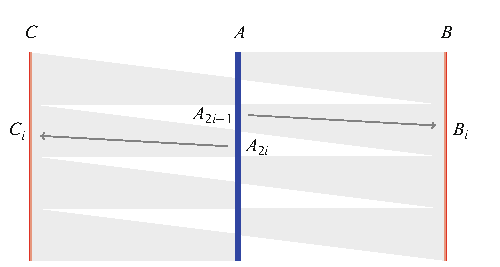
\includegraphics[width=.65\textwidth]{assets/fig-1-4-counterexample.pdf}
\end{center}

% 原书印刷21--25页，PDF物理49--53页.
\subsection{Kantorovich问题作为Monge问题的松弛}\label{sec:1.5}

再次令$K(\gamma):=\int_{\Omega\times\Omega}c\,d\gamma$. 我们知道，对任何映射$\mathrm{T}$，都有
\[
M(\mathrm{T})=\int_\Omega c(x,\mathrm{T}(x))\,d\mu
=\int_{\Omega\times\Omega}c\,d\gamma_\mathrm{T}=K(\gamma_\mathrm{T}),
\]
所以Monge问题可以改写为
\[
\min\{J(\gamma):\gamma\in\Pi(\mu,\nu)\},
\qquad
J(\gamma)=\begin{cases}
K(\gamma)=M(\mathrm{T}),&\gamma=\gamma_\mathrm{T},\\
+\infty,&\text{其他情形}.
\end{cases}
\]
这很容易理解：$J$的定义迫使最小化仅限于由传输映射诱导的计划. 这有助于把(MP)和(KP)视为定义在\emph{同一组可行对象}上的两个问题，唯一差别是待最小化的泛函为$J$还是$K$.

现在的问题是：Kantorovich为什么决定用$K$代替$J$？能否容易地证明$\inf K=\inf J$？如果$K$的极小元恰好形如$\gamma=\gamma_\mathrm{T}$，这当然成立，因为此时两个最小值相等. 但能否在一般情形下为这个过程提供依据？主要的数学依据来自下面的松弛概念.

\begin{sourcebox}{知识回顾：松弛}\label{box:1.10}
设$F:X\to\mathbb R\cup\{+\infty\}$是度量空间$X$上给定的有下界泛函. 我们把$F$的\emph{松弛}定义为泛函$\overline F:X\to\mathbb R\cup\{+\infty\}$：在所有下半连续且满足$G\le F$的泛函$G:X\to\mathbb R\cup\{+\infty\}$中，它是最大的一个. 这一泛函存在，因为任意一族下半连续函数的上确界仍然下半连续. 此外，我们还有一个容易证明的表示公式：
\[
\overline F(x)=\inf\{\liminf_n F(x_n):x_n\to x\}.
\]
定义还推出$\inf F=\inf\overline F$（后一项，即$\overline F$的下确界，在$X$紧时通常是最小值）. 这很容易验证：$F\ge\overline F$推出$\inf F\ge\inf\overline F$；另一方面，令$\ell:=\inf F$，则$F\ge\ell$，而常值函数是下半连续的. 因此$\overline F\ge\ell$，从而$\inf\overline F\ge\inf F$.
\end{sourcebox}

我们断言，在一定假设下，$K$正是$J$的松弛. 在这种情形中，这个松弛恰好不仅半连续，而且连续，并在$\{J<+\infty\}$上与$J$一致.

假设如下：取紧集$\Omega\subset\mathbb R^d$，假设$c$连续，$\mu$无原子（即对每个$x\in\Omega$，都有$\mu(\{x\})=0$）. 假设紧性是为了简化叙述，而结论在更一般的假设下也可能成立. 关于这一主题可参阅\cite{b253,b8}.

我们需要若干预备结果. 第一个涉及一维情形；我们会在\orig{86}{第2章}详细分析，但现在就可以陈述.

\begin{lemma}\label{obj:1.27}
若$\mu,\nu$是实直线$\mathbb R$上的两个概率测度，且$\mu$无原子，则至少存在一个传输映射$\mathrm{T}$满足$\mathrm{T}_\#\mu=\nu$.
\end{lemma}
\begin{proof}
只需考虑\autoref{obj:1.23}给出的单调递增映射$\mathrm{T}$. 这个映射还使二次成本最优，但这里我们并不关心这一点.
\end{proof}

\begin{lemma}\label{obj:1.28}
存在Borel映射$\sigma_d:\mathbb R^d\to\mathbb R$，它是单射，其像是$\mathbb R$的Borel子集，并且逆映射也是Borel可测的.
\end{lemma}
\begin{proof}
首先，只需对$d=2$证明结论，然后便可归纳：若已经给定$\mathbb R^{d-1}$上的映射$\sigma_{d-1}$，则可以令
\[
\sigma_d(x_1,x_2,\ldots,x_d)
=\sigma_2(x_1,\sigma_{d-1}(x_2,x_3,\ldots,x_d))
\]
构造$\sigma_d$.

其次，只需在$]0,1[^2$上定义这样的映射，因为可以用
\[
(x,y)\longmapsto
\left(\frac12+\frac1\pi\arctan x,\frac12+\frac1\pi\arctan y\right)
\]
从$\mathbb R^2$转到$]0,1[^2$.

然后，对十进制（或二进制）表示$x=0,x_1x_2x_3\ldots$与$y=0,y_1y_2y_3\ldots$，考虑把$(x,y)$送到$0,x_1y_1x_2y_2x_3y_3\ldots$的映射. 为避免歧义，我们约定不允许十进制表示以循环的$9$结尾（即$0.347299999\ldots$必须写成$0.3473$）. 因此，像不会是整个区间，例如$0.39393939\ldots$这样的点就无法通过该映射得到. 但这个点集确实是Borel可测的.

也不难验证该映射及其逆映射都是Borel可测的：通过指定实数前$2k$位数字所定义的每个区间，其原像恰是$\mathbb R^2$中的一个矩形，即分别指定两个分量前$k$位数字所定义的两个区间之积. 这些特殊区间构成Borel $\sigma$-代数的一组基，因而证明了所需的可测性.
\end{proof}

\begin{corollary}\label{obj:1.29}
若$\mu,\nu$是$\mathbb R^d$上的两个概率测度，且$\mu$无原子，则至少存在一个传输映射$\mathrm{T}$满足$\mathrm{T}_\#\mu=\nu$.
\end{corollary}
\begin{proof}
只需考虑从$(\sigma_d)_\#\mu$到$(\sigma_d)_\#\nu$的传输映射$\mathrm{T}$，然后与$\sigma_d$和$(\sigma_d)^{-1}$复合即可.
\end{proof}

\begin{remark}\label{obj:1.30}
这里，我们通过\autoref{obj:1.28}，给出了环境空间为$\mathbb R^d$时，在无原子测度$\mu$与任意测度$\nu$之间显式构造传输映射的方法. 事实上，这一事实要一般得多：众所周知，任何配备无原子测度的测度空间都与带Lebesgue测度的$[0,1]$同构.\footnote{注意，这正是\cite{b175}用来得到一般空间上传输映射存在性的论证；\cite{b253}指出，与把任意空间送到$[0,1]$的同构复合后，成本函数不再连续. 不过，可用\autoref{obj:1.8}处理，因为它允许使用如下形式的成本：连续函数与分别关于$x$和$y$的可测映射的复合.} 但当显式构造已足以处理欧氏情形、并满足我们的目的时，我们不想引入这类论证.
\end{remark}

最后还需要一个引理：

\begin{lemma}\label{obj:1.31}
设$X$是紧度量空间，配备概率测度$\varrho\in\mathscr P(X)$. 考虑划分序列$G_n$，其中每个$G_n$都是一族互不相交的子集$C_{i,n}$，对每个$n$都有$\bigcup_{i\in I_n}C_{i,n}=X$. 假设$\operatorname{size}(G_n):=\max_i\operatorname{diam}(C_{i,n})$在$n\to\infty$时趋于$0$，并考虑$X$上的概率测度序列$\varrho_n$，满足对每个$n$及$i\in I_n$都有$\varrho_n(C_{i,n})=\varrho(C_{i,n})$. 则$\varrho_n\rightharpoonup\varrho$.
\end{lemma}
\begin{proof}
令$m_{i,n}:=\varrho_n(C_{i,n})=\varrho(C_{i,n})$. 只需取连续函数$\phi\in C(X)$并注意到
\begin{equation*}
\begin{aligned}
\left|\int_X\phi\,d\varrho_n-\int_X\phi\,d\varrho\right|
&\le\sum_{i\in I_n}\left|\int_{C_{i,n}}\phi\,d\varrho_n-\int_{C_{i,n}}\phi\,d\varrho\right|\\
&\le\omega(\operatorname{diam}(C_{i,n}))\sum_{i\in I_n}m_{i,n}
=\omega(\operatorname{diam}(C_{i,n}))\to0,
\end{aligned}
\end{equation*}
其中$\omega$是$\phi$的连续模. 依据在于：当两个测度在集合$C\subset X$上具有相同质量时，由于$\phi$在该集合上的振幅不超过$\omega(\operatorname{diam}(C))$，两个积分之差至多为这个数乘以共同质量.

这证明$\int\phi\,d\varrho_n\to\int\phi\,d\varrho$，从而$\varrho_n\to\varrho$.
\end{proof}

现在可以证明以下结论.

\begin{theorem}\label{obj:1.32}
在紧子集$\Omega\subset\mathbb R^d$上，只要$\mu$无原子，由传输映射诱导的计划$\gamma_\mathrm{T}$组成的集合就在计划集$\Pi(\mu,\nu)$中稠密.
\end{theorem}
\begin{proof}
固定$n$，任取$\Omega$的一个划分，使各集合$K_{i,n}$的直径小于$1/(2n)$（例如小立方体）. 集合$C_{i,j,n}:=K_{i,n}\times K_{j,n}$构成$\Omega\times\Omega$的一个网格尺度小于$1/n$的划分.

现在任取测度$\gamma\in\Pi(\mu,\nu)$. 由\autoref{obj:1.31}，只需构造把$\mu$送到$\nu$的传输$\mathrm{T}$，使$\gamma_\mathrm{T}$在每个集合$C_{i,j,n}$上的质量都与$\gamma$相同. 为此，定义列$\operatorname{Col}_{i,n}:=K_{i,n}\times\Omega$，并以$\gamma_{i,n}$表示$\gamma$在$\operatorname{Col}_{i,n}$上的限制. 其边缘测度记为$\mu_{i,n}$与$\nu_{i,n}$. 对每个$i$，考虑把$\mu_{i,n}$送到$\nu_{i,n}$的传输映射$\mathrm{T}_{i,n}$. 由\autoref{obj:1.29}它存在，因为对每个$(i,n)$都有$\mu_{i,n}\le\mu$，所以这些测度无原子. 由于各$\mu_{i,n}$集中于互不相交的集合，把传输$\mathrm{T}_{i,n}$“粘合”起来便得到把$\mu$送到$\nu$的传输$\mathrm{T}$（这里使用了$\sum_i\mu_{i,n}=\mu$与$\sum_i\nu_{i,n}=\nu$）.

只需验证$\gamma_\mathrm{T}$在每个$C_{i,j,n}$上赋予与$\gamma$相同的质量，\footnote{注意，\cite{b8,b253}以更复杂的方式证明了同一事实；事实上，对每一列使用唯一一个传输映射就足够了. 相同想法也曾在\cite{b146}中用于另一个涉及Lipschitz传输映射的稠密性结果.}而这很容易. 事实上，这一质量等于$\gamma_{\mathrm{T}_{i,n}}$的相应质量，并且
\begin{equation*}
\begin{aligned}
\gamma_{\mathrm{T}_{i,n}}(C_{i,j,n})
&=\mu_{i,n}(\{x:x\in K_{i,n},\ \mathrm{T}_{i,n}(x)\in K_{j,n}\})\\
&=\mu_{i,n}(\{x:\mathrm{T}_{i,n}(x)\in K_{j,n}\})\\
&=\nu_{i,n}(K_{j,n})=\gamma(K_{i,n}\times K_{j,n}).
\end{aligned}
\end{equation*}
\end{proof}

松弛结论只是它的一个推论.

\begin{theorem}\label{obj:1.33}
在上述假设下，$K$是$J$的松弛. 特别地，$\inf J=\min K$，所以Monge问题与Kantorovich问题具有相同的下确界.
\end{theorem}
\begin{proof}
首先，由于$K$连续，它下半连续；又有$K\le J$，所以$K$必不大于$J$的松弛. 只需证明：对每个$\gamma$，都能找到传输序列$\mathrm{T}_n$，使$\gamma_{\mathrm{T}_n}\rightharpoonup\gamma$且$J(\gamma_{\mathrm{T}_n})\to K(\gamma)$，这样松弛泛函的序列刻画（见定义）中的下确界便不大于$K$，从而证明相等. 事实上，由于在$\gamma=\gamma_{\mathrm{T}_n}$时两个泛函$K,J$一致，而$K$连续，我们只需构造满足$\gamma_{\mathrm{T}_n}\rightharpoonup\gamma$的序列$\mathrm{T}_n$. 由\autoref{obj:1.32}这是可能的.
\end{proof}

% 原书印刷25--41页，PDF物理53--69页；结束于1.7标题之前.
\subsection[凸性、c-凹性、循环单调性、对偶与最优性]{凸性、$c$-凹性、循环单调性、对偶与最优性}\label{sec:1.6}

\subsubsection[凸函数与c-凹函数]{凸函数与$c$-凹函数}\label{sec:1.6.1}

本节把$c$-凹函数的性质与更为熟悉的凸函数作比较. 我们先回顾凸分析中的一些概念.

\begin{sourcebox}{知识回顾：凸函数}\label{box:1.11}
凸函数的定义始终相同：$f:\mathbb R^d\to\mathbb R\cup\{+\infty\}$是凸的，当且仅当对所有$x,y\in\mathbb R^d$及$t\in[0,1]$都有
\[
f((1-t)x+ty)\le(1-t)f(x)+tf(y).
\]
我们不特别讨论定义在子集$\Omega\subset\mathbb R^d$上的凸函数（为使定义有意义，$\Omega$应为凸集），因为总能在$\Omega$外令$f=+\infty$而将其延拓，同时保持凸性.

一个简单的稳定性性质如下：若$f_\alpha$是一族凸函数，那么由$f(x):=\sup_\alpha f_\alpha(x)$定义的$f$也凸. 只需写出
\[
f_\alpha((1-t)x+ty)\le(1-t)f_\alpha(x)+tf_\alpha(y)
\le(1-t)f(x)+tf(y)
\]
并对$\alpha$取上确界，就容易验证这一点. 也可以使用上图集（一个函数凸，当且仅当它的上图集凸），再注意到凸集之交仍然凸.

定义在$\mathbb R^d$上的实值凸函数自动连续且局部Lipschitz（一般地，它们在定义域$\{f<+\infty\}$的内部连续且局部Lipschitz）. 但在$\{f<+\infty\}$与$\{f=+\infty\}$的交界处可能不连续. 因而我们通常至少要求下半连续性.

\begin{theorem*}
函数$f:\mathbb R^d\to\mathbb R\cup\{+\infty\}$凸且下半连续，当且仅当存在一族仿射函数$f_\alpha$使$f(x):=\sup_\alpha f_\alpha(x)$. 这族函数也可取为所有不大于$f$的仿射函数.
\end{theorem*}

一个方向很容易（若$f$是仿射函数的上确界，由于仿射蕴含凸，所以$f$凸）. 逆命题背后的几何直觉在于：凸且下半连续函数的上图集是$\mathbb R^d\times\mathbb R$中的闭凸集，可写成所有包含它的半空间之交. 严格证明需要使用几何形式的Hahn--Banach定理.
\end{sourcebox}

\begin{sourcebox}{知识回顾：Legendre变换与次微分}\label{box:1.12}
\begin{definition*}[Legendre--Flenchel变换]
对任意给定函数$f:\mathbb R^d\to\mathbb R\cup\{+\infty\}$，可定义其变换
\[
f^*(y):=\sup_x x\cdot y-f(x).
\]
\end{definition*}
\begin{example*}
$x\mapsto\frac1p|x|^p$的Legendre变换是$x\mapsto\frac1q|x|^q$，其中$\frac1p+\frac1q=1$.
\end{example*}
函数$f$凸且下半连续，当且仅当存在$g$使$f=g^*$（因为某个函数的Legendre变换所组成的函数类，恰与可表示为仿射函数上确界的函数类一致）. 为说明每个仿射函数的上确界都能表示为$g^*$，只需取$f(y)=\sup_\alpha x_\alpha\cdot y+b_\alpha$；然后，对每个向量$x$，令$g(x)=-\sup\{b_\alpha:x_\alpha=x\}$（若没有$\alpha$满足$x_\alpha=x$，就令$g(x)=+\infty$），再验证$f=g^*$.

\begin{proposition*}
函数$f:\mathbb R^d\to\mathbb R\cup\{+\infty\}$凸且下半连续，当且仅当$f^{**}=f$.
\end{proposition*}
这一事实的证明可视为Hahn--Banach定理的应用. 完整证明（包括无限维情形）例如见\cite{b23}.

\begin{definition*}[次微分]
对每个凸函数$f$，定义其在$x$处的\emph{次微分}为集合
\[
\partial f(x)=\{p\in\mathbb R^d:f(y)\ge f(x)+p\cdot(y-x)\quad\forall y\in\mathbb R^d\}.
\]
\end{definition*}
可以证明，当$x$位于集合$\{f<+\infty\}$内部时，$\partial f(x)$总非空. 在$f$可微的每一点，$\partial f$退化为单点集$\{\nabla f\}$.

对于凸函数$f$及$f^*$的次微分，有
\[
p\in\partial f(x)\iff x\in\partial f^*(p)\iff f(x)+f^*(p)=x\cdot p.
\]
这有助于证明以下等价关系：取两个共轭函数$f,f^*$（其中$f=f^{**}$），则$f$为$C^1$，当且仅当$f^*$严格凸. 原因是，$C^1$意味着每个集合$\partial f(x)$中至多有一个$p$，而严格凸意味着同一个向量不能属于多于一个点处的次微分. 特别地，若$h$严格凸，则多值映射$\partial h$可求逆，逆映射单值，从而得到映射$(\partial h)^{-1}$；在\autoref{obj:1.17}的陈述中应使用这一映射代替$(\nabla h)^{-1}$.

最后，注意凸函数的次微分满足如下单调性：若$p_1\in\partial f(x_1)$且$p_2\in\partial f(x_2)$，则$(p_1-p_2)\cdot(x_1-x_2)\ge0$.
\end{sourcebox}

注意与$c$-凹函数（或$\bar c$-凹函数；在对称情形中这一区别没有意义）的类比：它们被定义为某个函数的$\bar c$-变换（或$c$-变换）. 事实上，除去符号的改变，$c$-凹性正是作为凸性的推广来定义的. 注意，我们允许凸函数取值$+\infty$，允许凹函数和$c$-凹函数取值$-\infty$. 但我们不希望凸函数恒等于$+\infty$，也不希望$c$-凹函数恒等于$-\infty$.

与其证明$f^{**}=f$这一结论，我们可以证明关于$c$-凹函数的如下更一般的结论.\footnote{注意，这一结果容易证明，因为$c$-凹函数恰被定义为某个函数的$c$-变换；而凸函数通常不是通过仿射函数的上确界来定义，而是通过凸性不等式来定义. 所以凸函数的对应定理通常需要使用Hahn--Banach定理.}

\begin{proposition}\label{obj:1.34}
假设$c$为实值函数. 对任意$\varphi:X\to\mathbb R\cup\{-\infty\}$，都有$\varphi^{c\bar c}\ge\varphi$. 等式$\varphi^{c\bar c}=\varphi$成立，当且仅当$\varphi$为$c$-凹函数；一般地，$\varphi^{c\bar c}$是不小于$\varphi$的最小$c$-凹函数.
\end{proposition}
\begin{proof}
先证明$\varphi^{c\bar c}\ge\varphi$. 写成
\begin{equation*}
\begin{aligned}
\varphi^{c\bar c}(x)
&=\inf_y c(x,y)-\varphi^c(y)\\
&=\inf_y c(x,y)-\inf_{x'}c(x',y)-\varphi(x').
\end{aligned}
\end{equation*}
考虑到$\inf_{x'}c(x',y)-\varphi(x')\le c(x,y)-\varphi(x)$，便有
\[
\varphi^{c\bar c}(x)\ge\inf_y c(x,y)-c(x,y)+\varphi(x)=\varphi(x).
\]
类似地，对任意$\zeta:Y\to\mathbb R\cup\{-\infty\}$，有$\zeta^{\bar c c}\ge\zeta$.

再证明当$\varphi$为$c$-凹函数时，$\varphi^{c\bar c}=\varphi$. 此时可写成
\[
\varphi=\zeta^{\bar c}
\implies\varphi^c=\zeta^{\bar c c}\ge\zeta
\implies\varphi^{c\bar c}\le\zeta^{\bar c}=\varphi,
\]
最后一个不等式来自$c$-变换与$\bar c$-变换会反转函数间的不等式（因为定义中有负号）. 因而，此时$\varphi^{c\bar c}\le\varphi$，从而$\varphi^{c\bar c}=\varphi$.

最后，证明对任意$\varphi$，函数$\varphi^{c\bar c}$是不小于$\varphi$的最小$c$-凹函数. 任取$c$-凹函数$\widetilde\varphi=\chi^{\bar c}$并假设$\widetilde\varphi\ge\varphi$. 则
\begin{equation*}
\begin{aligned}
\chi^{\bar c}\ge\varphi
&\implies\chi^{\bar c c}\le\varphi^c
\implies\chi\le\varphi^c\\
&\implies\widetilde\varphi=\chi^{\bar c}\ge\varphi^{c\bar c},
\end{aligned}
\end{equation*}
即得所需不等式.
\end{proof}

本小节最后介绍关于凸函数的一个概念，稍后再将其转到$c$-凹函数的框架.

把凸函数次微分的图定义为
\[
\operatorname{Graph}(\partial f):=\{(x,p):p\in\partial f(x)\}
=\{(x,p):f(x)+f^*(p)=x\cdot p\}.
\]
我们已经知道这个图是单调的，即对$i=1,2$有$(x_i,p_i)\in\operatorname{Graph}(\partial f)$时，
\[
(p_2-p_1)\cdot(x_2-x_1)\ge0.
\]
但并非所有单调图都是某个凸函数次微分的图，甚至未必包含在这样的图中.\footnote{例如，取$\mathbb R^2$中的$90^\circ$旋转$R$，并考虑集合$A=\{(x,Rx),x\in\mathbb R^d\}$. 它满足单调性不等式，因为对任意$x_1,x_2$都有$(Rx_1-Rx_2)\cdot(x_1-x_2)=0$. 但映射$x\mapsto Rx$不是凸函数的梯度（它根本不是梯度），也不可能包含在某个凸函数次微分的图中.}

所以，仅凭单调性不足以刻画凸函数的梯度和次微分（更确切地说，单调的梯度向量函数是凸函数的梯度，但单调性本身不能推出它是梯度）.

更强的概念是循环单调性.

\begin{definition}\label{obj:1.35}
若集合$A\subset\mathbb R^d\times\mathbb R^d$满足：对每个$k\in\mathbb N$、每个置换$\sigma$及任意有限组点$(x_1,p_1),\ldots,(x_k,p_k)\in A$，都有
\[
\sum_{i=1}^k x_i\cdot p_i\ge\sum_{i=1}^k x_i\cdot p_{\sigma(i)},
\]
则称$A$为\emph{循环单调的}.
\end{definition}

“循环”一词指的是：由于每个$\sigma$都是互不相交循环的复合，只对循环置换验证该性质就足够了，即在定义中用$\sum_{i=1}^k x_i\cdot p_{i+1}$代替$\sum_{i=1}^k x_i\cdot p_{\sigma(i)}$（自然约定$p_{k+1}=p_1$）.

注意，取$k=2$便得到通常的单调性定义，因为
\[
x_1\cdot p_1+x_2\cdot p_2\ge x_1\cdot p_2+x_2\cdot p_1
\iff(p_1-p_2)\cdot(x_1-x_2)\ge0.
\]
Rockafellar的一个著名定理（\cite{b260}，定理24.8）表明，每个循环单调集合都包含在某个凸函数次微分的图中. 这里不证明它，因为我们将把它视为关于$c$-凹函数的一个定理的特例.

\subsubsection[c-循环单调性与对偶]{$c$-循环单调性与对偶}\label{sec:1.6.2}

先把循环单调性的定义转到$c$-凹情形.

\begin{definition}\label{obj:1.36}
给定函数$c:X\times Y\to\mathbb R\cup\{+\infty\}$，若集合$\Gamma\subset X\times Y$满足：对每个$k\in\mathbb N$、每个置换$\sigma$及任意有限组点$(x_1,y_1),\ldots,(x_k,y_k)\in\Gamma$，都有
\[
\sum_{i=1}^k c(x_i,y_i)\le\sum_{i=1}^k c(x_i,y_{\sigma(i)}),
\]
则称$\Gamma$为\emph{$c$-循环单调的}（简称$c$-CM）.
\end{definition}

与凸情形一样，“循环”一词指的是只需考虑循环置换. “单调”一词则沿用自$c(x,y)=-x\cdot y$的情形.

值得回顾下面的定理，它推广了凸分析中Rockafellar的一个定理. 这一证明的经典参考文献是\cite{b269}，但有趣的是，它实际上可追溯到更早的论文，例如\cite{b261}（经济学中的行为可理性化框架，见该文定理1），或\cite{b91}（液晶的应用，作为距离成本下离散Kantorovich对偶性证明的一部分，见该文引理2）.

\begin{theorem}\label{obj:1.37}
若$\Gamma\ne\varnothing$是$X\times Y$中的$c$-CM集合，且$c:X\times Y\to\mathbb R$（注意，要求$c$不取值$+\infty$），则存在$c$-凹函数$\varphi:X\to\mathbb R\cup\{-\infty\}$（不恒等于$-\infty$）满足
\[
\Gamma\subset\{(x,y)\in X\times Y:\varphi(x)+\varphi^c(y)=c(x,y)\}.
\]
\end{theorem}
\begin{proof}
我们给出函数$\varphi$的显式公式，并证明其良定义且满足所要求的性质.

固定一点$(x_0,y_0)\in\Gamma$，对$x\in X$令
\begin{equation*}
\begin{aligned}
\varphi(x)=\inf\bigl\{&c(x,y_n)-c(x_n,y_n)+c(x_n,y_{n-1})-c(x_{n-1},y_{n-1})\\
&+\cdots+c(x_1,y_0)-c(x_0,y_0):\\
&n\in\mathbb N,\ (x_i,y_i)\in\Gamma\text{ 对所有 }i=1,\ldots,n\bigr\}.
\end{aligned}
\end{equation*}
由于$c$为实值且$\Gamma$非空，$\varphi$不取值$+\infty$.

若对$y\in Y$令
\begin{equation*}
\begin{aligned}
-\psi(y)=\inf\bigl\{&-c(x_n,y)+c(x_n,y_{n-1})-c(x_{n-1},y_{n-1})\\
&+\cdots+c(x_1,y_0)-c(x_0,y_0):\\
&n\in\mathbb N,\ (x_i,y_i)\in\Gamma\text{ 对所有 }i=1,\ldots,n,\ y_n=y\bigr\}.
\end{aligned}
\end{equation*}
由定义，$\psi(y)>-\infty$当且仅当$y\in(\pi_y)(\Gamma)$. 此外，由构造有$\varphi=\psi^{\bar c}$，这证明$\varphi$为$c$-凹函数.\footnote{注意，这里没有讨论$\varphi$的可测性：从其$c$-凹性可直接得到，因为它还是连续的，但这依赖于$c$一致连续的假设. 一般情形下，可测性和可积性更为棘手.} $\varphi$不恒等于$-\infty$可由$\varphi(x_0)\ge0$看出：事实上，取$x=x_0$，则对任意点链$(x_i,y_i)\in\Gamma$，都有
\[
\sum_{i=0}^n c(x_{i+1},y_i)\ge\sum_{i=0}^n c(x_i,y_i),
\]
这里约定$x_{n+1}=x_0$. 这表明$\varphi(x_0)$定义中的下确界非负.

为证明$\Gamma$上$\varphi(x)+\varphi^c(y)=c(x,y)$，只需证明同一集合上有$\varphi(x)+\varphi^c(y)\ge c(x,y)$，因为$c$-变换的定义总给出反向不等式. 此外，由$\varphi^c=\psi^{\bar c c}$及$\psi^{\bar c c}\ge\psi$，只需验证$\varphi(x)+\psi(y)\ge c(x,y)$.

设$(x,y)\in\Gamma$并固定$\varepsilon>0$. 由$\varphi=\psi^{\bar c}$，可找到$\bar y\in\pi_y(\Gamma)$使$c(x,\bar y)-\psi(\bar y)<\varphi(x)+\varepsilon$. 特别地，$\psi(\bar y)\ne\pm\infty$. 从$\psi$的定义得到$-\psi(y)\le-c(x,y)+c(x,\bar y)-\psi(\bar y)$（因为从$\bar y$出发的每条链都可通过添加点$(x,y)\in\Gamma$来补全）.

合并这些信息，得到
\[
-\psi(y)\le-c(x,y)+c(x,\bar y)-\psi(\bar y)
<-c(x,y)+\varphi(x)+\varepsilon.
\]
由于$\varepsilon$任意，这推出$c(x,y)\le\varphi(x)+\psi(y)$.
\end{proof}

现在可以证明以下结论.

\begin{theorem}\label{obj:1.38}
若$\gamma$是成本$c$下的最优传输计划，且$c$连续，则$\operatorname{spt}(\gamma)$是$c$-CM集合.
\end{theorem}
\begin{proof}
反设存在$k,\sigma$及$(x_1,y_1),\ldots,(x_k,y_k)\in\operatorname{spt}(\gamma)$，使
\[
\sum_{i=1}^k c(x_i,y_i)>\sum_{i=1}^k c(x_i,y_{\sigma(i)}).
\]
取$\varepsilon<\frac1{2k}\bigl(\sum_{i=1}^k c(x_i,y_i)-\sum_{i=1}^k c(x_i,y_{\sigma(i)})\bigr)$. 由$c$连续，存在$r$，使对所有$i=1,\ldots,k$及所有$(x,y)\in B(x_i,r)\times B(y_i,r)$都有$c(x,y)>c(x_i,y_i)-\varepsilon$，且对所有$(x,y)\in B(x_i,r)\times B(y_{\sigma(i)},r)$都有$c(x,y)<c(x_i,y_{\sigma(i)})+\varepsilon$.

令$V_i:=B(x_i,r)\times B(y_i,r)$. 因为$(x_i,y_i)\in\operatorname{spt}(\gamma)$，对每个$i$有$\gamma(V_i)>0$. 定义测度
\[
\gamma_i:=\frac{\gamma\mathbin{\vrule height 1.4ex depth -.3ex width .07ex\vrule height .07ex depth 0ex width .7ex}V_i}{\gamma(V_i)},
\qquad\mu_i:=(\pi_x)_\#\gamma_i,\quad\nu_i:=(\pi_y)_\#\gamma_i.
\]
取$\varepsilon_0<\frac1k\min_i\gamma(V_i)$.

对每个$i$任意构造测度$\widetilde\gamma_i\in\Pi(\mu_i,\nu_{\sigma(i)})$（例如取$\widetilde\gamma_i=\mu_i\otimes\nu_{\sigma(i)}$）. 定义
\[
\widetilde\gamma:=\gamma-\varepsilon_0\sum_{i=1}^k\gamma_i
+\varepsilon_0\sum_{i=1}^k\widetilde\gamma_i.
\]
我们要证明$\widetilde\gamma$在传输问题中比$\gamma$更优，即$\widetilde\gamma\in\Pi(\mu,\nu)$且$\int c\,d\widetilde\gamma<\int c\,d\gamma$，从而得到矛盾.

首先验证$\widetilde\gamma$为正测度. 只需验证$\gamma-\varepsilon_0\sum_{i=1}^k\gamma_i$为正，为此条件$\varepsilon_0\gamma_i<\frac1k\gamma$就足够. 这一条件成立，因为$\varepsilon_0\gamma_i=(\varepsilon_0/\gamma(V_i))\gamma\mathbin{\vrule height 1.4ex depth -.3ex width .07ex\vrule height .07ex depth 0ex width .7ex}V_i$且$\varepsilon_0/\gamma(V_i)\le1/k$.

再验证$\widetilde\gamma$的边缘条件. 有
\begin{equation*}
\begin{aligned}
(\pi_x)_\#\widetilde\gamma
&=\mu-\varepsilon_0\sum_{i=1}^k(\pi_x)_\#\gamma_i
+\varepsilon_0\sum_{i=1}^k(\pi_x)_\#\widetilde\gamma_i\\
&=\mu-\varepsilon_0\sum_{i=1}^k\mu_i+\varepsilon_0\sum_{i=1}^k\mu_i=\mu,\\
(\pi_y)_\#\widetilde\gamma
&=\nu-\varepsilon_0\sum_{i=1}^k(\pi_y)_\#\gamma_i
+\varepsilon_0\sum_{i=1}^k(\pi_y)_\#\widetilde\gamma_i\\
&=\nu-\varepsilon_0\sum_{i=1}^k\nu_i+\varepsilon_0\sum_{i=1}^k\nu_{\sigma(i)}=\nu.
\end{aligned}
\end{equation*}
最后估计$\int c\,d\gamma-\int c\,d\widetilde\gamma$并证明它为正，便结束证明. 有
\begin{equation*}
\begin{aligned}
\int c\,d\gamma-\int c\,d\widetilde\gamma
&=\varepsilon_0\sum_{i=1}^k\int c\,d\gamma_i
-\varepsilon_0\sum_{i=1}^k\int c\,d\widetilde\gamma_i\\
&\ge\varepsilon_0\sum_{i=1}^k(c(x_i,y_i)-\varepsilon)
-\varepsilon_0\sum_{i=1}^k(c(x_i,y_{\sigma(i)})+\varepsilon)\\
&=\varepsilon_0\left(\sum_{i=1}^k c(x_i,y_i)
-\sum_{i=1}^k c(x_i,y_{\sigma(i)})-2k\varepsilon\right)>0.
\end{aligned}
\end{equation*}
这里使用了：$\gamma_i$集中于$B(x_i,r)\times B(y_i,r)$，$\widetilde\gamma_i$集中于$B(x_i,r)\times B(y_{\sigma(i)},r)$，并且它们质量为$1$（因为已除以$\gamma(V_i)$进行缩放）.
\end{proof}

由上一条定理以及\autoref{obj:1.37}，便得到我们从\autoref{sec:1.2}以来一直等待的对偶结论.\footnote{我们强调，这只是一条可能的路线：这里通过循环单调性证明对偶；也可以先证明对偶（见\autoref{sec:1.6.3}），再通过\autoref{obj:1.42}那样的论证证明循环单调性.}

\begin{theorem}\label{obj:1.39}
设$X,Y$是Polish空间，$c:X\times Y\to\mathbb R$一致连续且有界. 则问题(DP)存在解$(\varphi,\varphi^c)$，并且$\max(\mathrm{DP})=\min(\mathrm{KP})$.
\end{theorem}
\begin{proof}
先考虑最小化问题(KP). 由于$c$连续，它存在解$\gamma$. 此外，由\autoref{obj:1.38}，$\gamma$的支集$\Gamma$是$c$-循环单调的. 由于$c$为实值，可应用\autoref{obj:1.37}，得到一个$c$-凹函数$\varphi$满足
\[
\Gamma\subset\{(x,y)\in\Omega\times\Omega:\varphi(x)+\varphi^c(y)=c(x,y)\}.
\]
由$c$-凹性（及$\bar c$-凹性），$\varphi,\varphi^c$连续. 此外，由$\varphi^c(y)=\inf_x c(x,y)-\varphi(x)$可得$\varphi^c$的上界（因为假设$c$有界），再转为$\varphi$的下界. 对称地，也能得到$\varphi$的上界和$\varphi^c$的下界，故两者都连续且有界.

因此，$(\varphi,\varphi^c)$可作为(DP)中的可行对. 现在考虑
\begin{equation*}
\begin{aligned}
\int_X\varphi\,d\mu+\int_Y\varphi^c\,d\nu
&=\int_{X\times Y}(\varphi(x)+\varphi^c(y))\,d\gamma\\
&=\int_{X\times Y}c(x,y)\,d\gamma.
\end{aligned}
\end{equation*}
最后一个等式是因为$\gamma$集中于$\Gamma$，其上有$\varphi(x)+\varphi^c(y)=c(x,y)$. 前一个等式则来自$\gamma$的边缘测度分别为$\mu,\nu$. 利用$\gamma$的最优性，最终得到
\[
(\mathrm{DP})\ge\int\varphi\,d\mu+\int\varphi^c\,d\nu
=\int c(x,y)\,d\gamma=(\mathrm{KP}),
\]
从而推出$(\mathrm{DP})=(\mathrm{KP})$，因为我们已知$(\mathrm{DP})\le(\mathrm{KP})$. 证明同时说明，$(\varphi,\varphi^c)$是(DP)的最优对.
\end{proof}

我们还希望处理上一条定理未涵盖的若干情形. 首先，为呼应\autoref{sec:1.3.1}，给出关于$\mathbb R^d$上二次情形的一个简短陈述. 与\autoref{obj:1.39}相比，区别在于成本$c(x,y)=\frac12|x-y|^2$既不有界，也不一致连续.

\begin{theorem}\label{obj:1.40}
设$\mu,\nu$是$\mathbb R^d$上的概率测度，$c(x,y)=\frac12|x-y|^2$. 假设$\int|x|^2\,dx,\int|y|^2\,dy<+\infty$. 考虑(DP)的如下变体：
\begin{equation*}\tag{DP-var}\label{eq:DP-var}
\begin{aligned}
\sup\biggl\{&\int_{\mathbb R^d}\varphi\,d\mu+\int_{\mathbb R^d}\psi\,d\nu:\\
&\varphi\in L^1(\mu),\ \psi\in L^1(\nu),\ \varphi\oplus\psi\le c\biggr\}.
\end{aligned}
\end{equation*}
则\eqref{eq:DP-var}存在解$(\varphi,\psi)$，而函数$x\mapsto\frac12|x|^2-\varphi(x)$与$y\mapsto\frac12|y|^2-\psi(y)$都是凸函数，且互为Legendre变换的共轭. 此外，$\max(\mathrm{DP\text{-}var})=\min(\mathrm{KP})$.
\end{theorem}
\begin{proof}
应用与\autoref{obj:1.39}相同的论证，可得一对函数$(\varphi,\psi)$，其中$\varphi$为$c$-凹函数、$\psi=\varphi^c$，并且最优传输计划$\gamma$支集中的每个$(x,y)$都满足$\varphi(x)+\varphi^c(y)=c(x,y)$. 由\autoref{obj:1.21}可得，$x\mapsto\frac12|x|^2-\varphi(x)$与$y\mapsto\frac12|y|^2-\psi(y)$凸且互相共轭. 特别地，$\frac12|x|^2-\varphi(x)$被一个线性函数从下方控制，故$\varphi$被一个二次多项式从上方控制. 由对$\mu$的假设，这证明$\varphi_+\in L^1(\mu)$. 对$\psi$也同样成立，即$\psi_+\in L^1(\nu)$. 现在可以对$\varphi\oplus\psi$关于$\gamma$积分，得到
\begin{equation*}
\begin{aligned}
\int_{\mathbb R^d}\varphi\,d\mu+\int_{\mathbb R^d}\psi\,d\nu
&=\int_{\mathbb R^d\times\mathbb R^d}\varphi\oplus\psi\,d\gamma\\
&=\int_{\mathbb R^d\times\mathbb R^d}c\,d\gamma\ge0.
\end{aligned}
\end{equation*}
这证明$\int_{\mathbb R^d}\varphi\,d\mu,\int_{\mathbb R^d}\psi\,d\nu>-\infty$，故$\varphi\in L^1(\mu)$且$\psi\in L^1(\nu)$.

随后如前便可得结论.
\end{proof}

接下来，对$c$不连续、而只下半连续的情形也作一些说明. 回顾，这一假设足以保证最优传输计划存在.

第一个结果涉及对偶公式的有效性，即
\begin{equation}\label{eq:1.6}
\begin{aligned}
\min(\mathrm{KP})=\sup\biggl\{&\int_X\varphi\,d\mu+\int_Y\psi\,d\nu:\\
&\varphi\in C(X),\ \psi\in C(Y),\ \varphi\oplus\psi\le c\biggr\}.
\end{aligned}
\end{equation}
到目前为止，我们在$c$一致连续且有界时证明了这一等式，同时还证明对偶问题存在一个达到最大值的函数对. 还知道一个不等式总成立：左侧最小值总不小于右侧最大值. 更确切地说，我们能够处理一致连续的情形（因为希望保证形如$\varphi(x)=\inf_y c(x,y)-\psi(y)$的$c$-凹函数连续）.

为处理有下界的下半连续成本$c$，我们使用如下事实：存在连续函数序列$c_k$（每个都是$k$-Lipschitz的）单调递增地收敛到$c$. 需要下面的引理.

\begin{lemma}\label{obj:1.41}
假设$c_k,c$下半连续且有下界，$c_k$单调递增地收敛到$c$. 则
\begin{equation*}
\begin{aligned}
&\lim_{k\to\infty}\min\left\{\int c_k\,d\gamma:\gamma\in\Pi(\mu,\nu)\right\}\\
&\qquad=\min\left\{\int c\,d\gamma:\gamma\in\Pi(\mu,\nu)\right\}.
\end{aligned}
\end{equation*}
\end{lemma}
\begin{proof}
由单调递增收敛条件，有$c_k\le c$，所以左侧极限（由单调性而存在）显然不大于右侧的量. 现在，对每个成本$c_k$选取一个最优解，构成序列$\gamma_k\in\Pi(\mu,\nu)$. 由$\Pi(\mu,\nu)$的紧性，可以在取子列后假设$\gamma_k\rightharpoonup\bar\gamma$. 固定一个指标$j$. 对$k\ge j$有$c_k\ge c_j$，因此
\begin{equation*}
\begin{aligned}
&\lim_k\min\left\{\int c_k\,d\gamma:\gamma\in\Pi(\mu,\nu)\right\}\\
&\qquad=\lim_k\int c_k\,d\gamma_k
\ge\liminf_k\int c_j\,d\gamma_k.
\end{aligned}
\end{equation*}
由积分成本$c_j$的半连续性，
\[
\liminf_k\int c_j\,d\gamma_k\ge\int c_j\,d\bar\gamma.
\]
于是得到
\[
\lim_k\min\left\{\int c_k\,d\gamma,\ \gamma\in\Pi(\mu,\nu)\right\}
\ge\int c_j\,d\bar\gamma.
\]
由于$j$任意，而由单调收敛有$\lim_j\int c_j\,d\bar\gamma=\int c\,d\bar\gamma$，我们还有
\begin{equation*}
\begin{aligned}
&\lim_k\min\left\{\int c_k\,d\gamma,\ \gamma\in\Pi(\mu,\nu)\right\}\\
&\qquad\ge\int c\,d\bar\gamma
\ge\min\left\{\int c\,d\gamma,\ \gamma\in\Pi(\mu,\nu)\right\}.
\end{aligned}
\end{equation*}
证明完毕. 注意，这还同时给出$\bar\gamma$对于极限成本$c$的最优性.
\end{proof}

现在可以确立半连续成本下对偶公式的有效性.

\begin{theorem}\label{obj:1.42}
若$X,Y$是Polish空间，$c:X\times Y\to\mathbb R\cup\{+\infty\}$下半连续且有下界，则对偶公式$\min(\mathrm{KP})=\sup(\mathrm{DP})$成立.
\end{theorem}
\begin{proof}
考虑由$k$-Lipschitz函数组成、单调递增地逼近$c$的序列$c_k$. 同一对偶公式对$c_k$成立，因而有
\begin{equation*}
\begin{aligned}
\min\left\{\int c_k\,d\gamma:\gamma\in\Pi(\mu,\nu)\right\}
&=\max\left\{\int\varphi\,d\mu+\int\psi\,d\nu:\varphi\oplus\psi\le c_k\right\}\\
&\le\sup\left\{\int\varphi\,d\mu+\int\psi\,d\nu:\varphi\oplus\psi\le c\right\},
\end{aligned}
\end{equation*}
其中最大值和上确界都是在$C_b$函数$\varphi,\psi$中计算的. 不等式来自$c_k\le c$，因此满足$\varphi(x)+\psi(y)\le c_k(x,y)$的每一对$(\varphi,\psi)$也满足$\varphi(x)+\psi(y)\le c(x,y)$. 令$k\to+\infty$，由\autoref{obj:1.41}便得结论. 注意，对成本$c$不能保证存在达到最大值的函数对$(\varphi,\psi)$.
\end{proof}

对偶公式也允许证明下面的$c$-循环单调性定理.

\begin{theorem}\label{obj:1.43}
若$c$下半连续且$\gamma$为最优传输计划，则$\gamma$集中于某个$c$-CM集合$\Gamma$（一般而言该集合不闭）.
\end{theorem}
\begin{proof}
由上一条定理，对偶公式成立. 这意味着在对偶问题中取一个极大化函数对序列$(\varphi_h,\psi_h)$，就有
\begin{equation*}
\begin{aligned}
\int(\varphi_h(x)+\psi_h(y))\,d\gamma
&=\int\varphi_h\,d\mu+\int\psi_h\,d\nu\\
&\longrightarrow\int c\,d\gamma,
\end{aligned}
\end{equation*}
因为$\int c\,d\gamma$是原问题的最小值，也就是对偶问题的最大值. 此外，有$c(x,y)-\varphi_h(x)+\psi_h(y)\ge0$；这意味着定义在$X\times Y$上的函数$f_h:=c(x,y)-\varphi_h(x)-\psi_h(y)$在$L^1(X\times Y;\gamma)$中收敛到$0$（因为它们非负，且积分趋于$0$）. 因此，取一个不重新编号的子列后，它们还$\gamma$-几乎处处逐点收敛到$0$. 设$\Gamma\subset X\times Y$是一个$\gamma(\Gamma)=1$且其上该收敛成立的集合.

任取$k,\sigma$以及$(x_1,y_1),\ldots,(x_k,y_k)\in\Gamma$，有
\begin{equation*}
\begin{aligned}
\sum_{i=1}^k c(x_i,y_i)
&=\lim_h\sum_{i=1}^k\varphi_h(x_i)+\psi_h(y_i)\\
&=\lim_h\sum_{i=1}^k\varphi_h(x_i)+\psi_h(y_{\sigma(i)})\\
&\le\sum_{i=1}^k c(x_i,y_{\sigma(i)}),
\end{aligned}
\end{equation*}
这证明该集合为$c$-CM.
\end{proof}

\begin{remark}\label{obj:1.44}
我们对下半连续成本$c$证明的对偶公式与连续成本下的公式不同之处在于：对偶问题(DP)未必存在解. 事实上，若按\eqref{eq:DP-var}重新表述对偶问题，就能先应用\autoref{obj:1.43}，说明最优$\gamma$集中于某个$c$-CM集合$\Gamma$，再通过\autoref{obj:1.37}构造势$\varphi$，从而得到最优解. 这在$c$为实值的假设下成立，不依赖其连续性.\footnote{但要注意，这一构造需要使用最优$\gamma$；当$c$下半连续时其存在性有保证，在某些特殊情形也可能存在，例如可以应用\autoref{obj:1.8}时. 此外，对非一致连续的成本$c$，\autoref{obj:1.37}中的函数$\varphi$存在可测性问题.}
\end{remark}

\subsubsection{对偶性的一个直接证明}\label{sec:1.6.3}

在\autoref{sec:1.6.2}中，我们偿还了\autoref{sec:1.2}欠下的对偶性之债：借助$c$-循环单调性论证，在相当一般的假设下证明了$\min(\mathrm{KP})=\sup(\mathrm{DP})$，没有对偶间隙.

这里给出另一个证明，它不依赖$c$-循环单调性，而是基于一个简单的凸分析技巧.\footnote{虽然并非严格必要，我们仍愿为完整性而给出这一证明；它也不同于其他文献，例如\cite{b292}的论证，其中主要工具是\cite{b90}第1章的一个定理，应用于恰当选取的函数与空间. 这里的证明由C. Jimenez建议，本质上改编自\cite{b70}第4节.} 我们限于紧的情形，并只使用以下事实：若$H$凸且下半连续，则$H^{**}=H$（见\autoref{sec:1.6.1}中的\autoref{box:1.12}）.

假设$X,Y$为紧度量空间，$c:X\times Y\to\mathbb R$连续. 对每个$p\in C(X\times Y)$，定义
\begin{equation*}
\begin{aligned}
H(p):=-\max\biggl\{&\int_X\varphi\,d\mu+\int_Y\psi\,d\nu:\\
&\varphi(x)+\psi(y)\le c(x,y)-p(x,y)\biggr\}.
\end{aligned}
\end{equation*}
它等于成本$c-p$下(DP)的值的相反数. 此值可取到已由\autoref{obj:1.11}证明；该命题也给出了最优$\varphi,\psi$的连续模界（与$c-p$相同）以及振幅界（若令$\varphi(x_0)=0$，那么$\varphi,\psi$都被一个仅依赖$\sup|c-p|$的常数控制）.

\begin{lemma}\label{obj:1.45}
函数$H:C(X\times Y)\to\mathbb R$凸，且关于紧空间$X\times Y$上的一致收敛下半连续.
\end{lemma}
\begin{proof}
先证明凸性. 取$p_0,p_1$及其最优势$(\varphi_0,\psi_0)$与$(\varphi_1,\psi_1)$. 对$t\in[0,1]$，定义$p_t=(1-t)p_0+tp_1$、$\varphi_t=(1-t)\varphi_0+t\varphi_1$及$\psi_t=(1-t)\psi_0+t\psi_1$. 函数对$(\varphi_t,\psi_t)$在定义$-H(p_t)$的最大化问题中可行. 因而
\[
H(p_t)\le-\left(\int_X\varphi_t\,d\mu+\int_Y\psi_t\,d\nu\right)
=(1-t)H(p_0)+tH(p_1),
\]
这证明凸性.

对半连续性，取$p_n\to p$. 抽取实现$H(p_n)$的下极限的子列$p_{n_k}$. 由一致收敛，序列$p_{n_k}$等度连续且有界（使用Ascoli--Arzel\`a定理的逆命题）. 因此，对应的最优势$(\varphi_{n_k},\psi_{n_k})$也等度连续且有界；再抽取子列后，可假设$\varphi_{n_k}\to\varphi$、$\psi_{n_k}\to\psi$一致成立. 显然，由$\varphi_{n_k}(x)+\psi_{n_k}(y)\le c(x,y)-p_{n_k}(x,y)$可得$\varphi(x)+\psi(y)\le c(x,y)-p(x,y)$. 故
\begin{equation*}
\begin{aligned}
H(p)&\le-\left(\int_X\varphi\,d\mu+\int_Y\psi\,d\nu\right)\\
&=\lim_k H(p_{n_k})=\liminf_n H(p_n),
\end{aligned}
\end{equation*}
这证明下半连续性.
\end{proof}

现在计算$H^*:\mathscr M(X\times Y)\to\mathbb R\cup\{+\infty\}$. 对$\gamma\in\mathscr M(X\times Y)$，有
\begin{equation*}
\begin{aligned}
H^*(\gamma):={}&\sup_p\int_{X\times Y}p\,d\gamma\\
&+\sup\left\{\int_X\varphi\,d\mu+\int_Y\psi\,d\nu:
\varphi(x)+\psi(y)\le c(x,y)-p(x,y)\right\}.
\end{aligned}
\end{equation*}
它可写成对$p,\varphi,\psi$统一取一次上确界的形式. 注意，若$\gamma\notin\mathscr M_+(X\times Y)$，则存在$p\le0$使$\int p_0\,d\gamma>0$；可取$\varphi=0$、$\psi=0$、$p=c+np_0$，并令$n\to\infty$，便得$H^*(\gamma)=+\infty$. 相反，若$\gamma\in\mathscr M_+(X\times Y)$，则应选取尽可能大的$p$，即$p(x,y)=c(x,y)-\varphi(x)-\psi(y)$. 这给出
\begin{equation*}
\begin{aligned}
H^*(\gamma)=\sup_{\varphi,\psi}\biggl(&\int_{X\times Y}c(x,y)\,d\gamma
+\int_X\varphi\,d\mu-\int_{X\times Y}\varphi(x)\,d\gamma\\
&+\int_Y\psi\,d\nu-\int_{X\times Y}\psi(x)\,d\gamma\biggr).
\end{aligned}
\end{equation*}
但这正是\autoref{sec:1.2}中为改写(KP)的约束而引入的表达式（见\eqref{eq:1.3}）. 事实上，
\[
H^*(\gamma)=\begin{cases}
K(\gamma),&\gamma\in\Pi(\mu,\nu),\\
+\infty,&\text{其他情形}.
\end{cases}
\]
于是得到对偶定理.

\begin{theorem}\label{obj:1.46}
若$X,Y$为紧空间且$c$连续，则$\min(\mathrm{KP})=\sup(\mathrm{DP})$（凸分析证明）.
\end{theorem}
\begin{proof}
有$\max(\mathrm{DP})=-H(0)=-H^{**}(0)$（因为$H$凸且下半连续，见\autoref{box:1.12}）. 此外，
\[
H^{**}(0)=\sup_\gamma\langle0,\gamma\rangle-H^*(\gamma)
=-\inf H^*=-\min(\mathrm{KP}).
\]
\end{proof}

\subsubsection{最优性的充分条件与稳定性}\label{sec:1.6.4}

\autoref{sec:1.6.1}和\autoref{sec:1.6.2}中关于$c$-变换的讨论，使我们能够证明最优传输中的最优性充分条件，至少当成本满足\autoref{obj:1.16}的扭转条件时如此. 与\autoref{sec:1.3}一样，先在紧性假设下给出一般陈述，再对二次情形给出不需要紧性的另一证明.

\begin{theorem}\label{obj:1.47}
设$\Omega\subset\mathbb R^d$紧，$c$为在$\Omega\times\Omega$上满足扭转条件的$C^1$成本函数. 给定$\mu\in\mathscr P(\Omega)$与$\varphi\in c\text{-}\operatorname{conc}(\Omega)$，假设$\varphi$在$\mu$-几乎处处可微，且$\mu(\partial\Omega)=0$. 假设映射$\mathrm{T}$满足$\nabla_xc(x,\mathrm{T}(x))=\nabla\varphi(x)$. 则$\mathrm{T}$对于测度$\mu$与$\nu:=\mathrm{T}_\#\mu$之间的传输成本$c$是最优的.
\end{theorem}
\begin{proof}
考虑函数$\varphi$，它可写成$\varphi(x)=\inf_y c(x,y)-\psi(y)$，其中$\psi:\Omega\to\mathbb R$为某个函数. 可假设$\psi$为$\bar c$-凹函数，因而连续（事实上，由上一小节的讨论可取$\psi=\varphi^c$）. 固定$x_0\in\Omega$，使$\nabla\varphi(x_0)$存在且$x_0\notin\partial\Omega$. 由紧性与连续性，下确界$\inf_y c(x,y)-\psi(y)$在某点$y_0$取到. 这给出
\[
\varphi(x)\le h(x-y_0)-\psi(y_0)\quad\text{对每个 }x,
\qquad\varphi(x_0)=h(x_0-y_0)-\psi(y_0).
\]
因此$x\mapsto h(x-y_0)-\varphi(x)$在$x=x_0$处取最小值（注意，我们通过关于$y$的最优性定义了$y_0$，但现在使用关于$x$的最优性）. 因而
\[
\nabla\varphi(x_0)=\nabla_xc(x_0,y_0).
\]
由假设，$y\mapsto\nabla_xc(x_0,y)$为单射，这推出$y_0=\mathrm{T}(x_0)$. 所以$\varphi(x_0)+\psi(\mathrm{T}(x_0))=c(x_0,\mathrm{T}(x_0))$，且同一等式对$\mu$-几乎处处的$x_0$成立. 对$\mu$积分得到
\begin{equation*}
\begin{aligned}
\int\varphi\,d\mu+\int\psi\,d\nu
&=\int\varphi\,d\mu+\int\psi\circ \mathrm{T}\,d\mu\\
&=\int c(x,\mathrm{T}(x))\,d\mu(x).
\end{aligned}
\end{equation*}
这证明$\mathrm{T}$最优，因为最后一个积分就是Monge问题中$\mathrm{T}$的成本，而由于$(\varphi,\psi)$在(DP)中可行，有$\int\varphi\,d\mu+\int\psi\,d\nu\le(\mathrm{DP})\le(\mathrm{KP})$.
\end{proof}

按照先前的约定，下面对$c(x,y)=\frac12|x-y|^2$给出另一证明.

\begin{theorem}\label{obj:1.48}
设$\mu\in\mathscr P(\mathbb R^d)$满足$\int|x|^2\,d\mu(x)<\infty$，且$u:\mathbb R^d\to\mathbb R\cup\{+\infty\}$凸并在$\mu$-几乎处处可微. 令$\mathrm{T}=\nabla u$，并假设$\int|\mathrm{T}(x)|^2\,d\mu(x)<+\infty$. 则对于测度$\mu$与$\nu:=\mathrm{T}_\#\mu$之间的传输成本$c(x,y):=\frac12|x-y|^2$，$\mathrm{T}$是最优的.
\end{theorem}
\begin{proof}
首先注意，对凸函数$u$有以下性质：
\[
\begin{aligned}
u(x)+u^*(y)&\ge x\cdot y&&\text{对所有 }x,y\in\mathbb R^d,\\
u(x)+u^*(y)&=x\cdot y&&\text{若 }y=\nabla u(x).
\end{aligned}
\]
现在，任取传输计划$\gamma\in\Pi(\mu,\nu)$，写出
\begin{equation*}
\begin{aligned}
\int_{\mathbb R^d\times\mathbb R^d}(x\cdot y)\,d\gamma(x,y)
&\le\int_{\mathbb R^d\times\mathbb R^d}(u(x)+u^*(y))\,d\gamma(x,y)\\
&=\int_{\mathbb R^d}u(x)\,d\mu(x)
+\int_{\mathbb R^d}u^*(\mathrm{T}(x))\,d\mu(x)\\
&=\int_{\mathbb R^d}(x\cdot \mathrm{T}(x))\,d\mu(x).
\end{aligned}
\end{equation*}
这证明$\int(x\cdot y)\,d\gamma\le\int(x\cdot y)\,d\gamma_\mathrm{T}$. 从仅依赖于$\mu,\nu$的积分
\[
\int\frac12(|x|^2+|y|^2)\,d\gamma
=\int\frac12(|x|^2+|y|^2)\,d\gamma_\mathrm{T}
\]
中减去这些量，便得
\[
\int_{\mathbb R^d\times\mathbb R^d}\frac12|x-y|^2\,d\gamma
\ge\int_{\mathbb R^d\times\mathbb R^d}\frac12|x-y|^2\,d\gamma_\mathrm{T},
\]
即得结论.
\end{proof}

对刚给出的两个不同证明再作一点说明：我们需要证明点$\mathrm{T}(x)$在所有可能的点$y$中具有某些最优性. 第一种情形中，我们先证明存在最优点$y_0$，再从一阶最优性条件推出$y_0=\mathrm{T}(x_0)$. 第二种情形中，我们使用凸函数极小元的刻画：梯度为零的点总是极小元. 这正是“若$y=\nabla u(x)$则$u(x)+u^*(y)=x\cdot y$”这一性质背后的想法.

现在转向几乎任意成本都可使用的更一般判据. 主要想法是：我们已证明最优计划必集中于$c$-CM集合，但逆命题也成立——集中于$c$-CM集合的计划是最优的，至少在最合理的情形下如此. 我们在最简单的情形，即$c$一致连续且有界时证明这一点. 实际上，从下一个证明可见，主要工具是\autoref{obj:1.37}，它只要求成本有限；但为避免可积性问题，需要连续性与紧性（此时所有函数都可测且有界）. 此外，我们会把这一充分条件用于另一个有趣的问题，即最优计划的稳定性；这还会由于其他原因而需要这些假设. 去掉这些假设后（特别是允许成本取无穷值时），逆命题是否仍成立是一个微妙的问题：成本取值$+\infty$时的反例见\cite{b10}，而若干有趣的肯定结果证明见\cite{b30,b60,b254}.

\begin{theorem}\label{obj:1.49}
给定$\gamma\in\mathscr P(X\times Y)$，假设$X,Y$为Polish空间，$c:X\times Y\to\mathbb R$一致连续且有界，并且$\operatorname{spt}(\gamma)$为$c$-CM集合. 则$\gamma$是其边缘测度$\mu=(\pi_x)_\#\gamma$与$\nu=(\pi_y)_\#\gamma$之间、成本为$c$的最优传输计划.
\end{theorem}
\begin{proof}
\autoref{obj:1.37}保证存在$c$-凹函数$\varphi$，使$\operatorname{spt}(\gamma)$包含于集合$\{(x,y):\varphi(x)+\varphi^c(y)=c(x,y)\}$. 由$c$的连续性，$\varphi,\varphi^c$都连续，因此分别在$X,Y$上有界.

由已知的对偶性质，
\begin{equation*}
\begin{aligned}
(\mathrm{KP})&\le\int c(x,y)\,d\gamma
=\int(\varphi(x)+\varphi^c(y))\,d\gamma\\
&=\int\varphi\,d\mu+\int\varphi^c\,d\nu
\le(\mathrm{DP})=(\mathrm{KP}),
\end{aligned}
\end{equation*}
这表明$\gamma$最优（且$(\varphi,\varphi^c)$求解了对偶问题）.
\end{proof}

现在能够证明下面的稳定性结果；这里只陈述紧的情形.

\begin{theorem}\label{obj:1.50}
设$X,Y$为紧度量空间，$c:X\times Y\to\mathbb R$连续. 假设$\gamma_n\in\mathscr P(X\times Y)$是一列传输计划，对成本$c$，它们都是各自边缘测度$\mu_n:=(\pi_x)_\#\gamma_n$与$\nu_n:=(\pi_y)_\#\gamma_n$之间的最优计划，并且$\gamma_n\rightharpoonup\gamma$. 则$\mu_n\rightharpoonup\mu:=(\pi_x)_\#\gamma$、$\nu_n\rightharpoonup\nu:=(\pi_y)_\#\gamma$，而$\gamma$是$\mu$与$\nu$之间的最优传输.
\end{theorem}
\begin{proof}
令$\Gamma_n:=\operatorname{spt}(\gamma_n)$. 取子列后，可假设$\Gamma_n\to\Gamma$关于Hausdorff拓扑成立（见下文）. 由\autoref{obj:1.38}，每个支集$\Gamma_n$都是$c$-CM集合；而$c$-CM集合的Hausdorff极限仍是$c$-CM的. 事实上，固定$(x_1,y_1),\ldots,(x_k,y_k)\in\Gamma$，则存在点$(x_1^n,y_1^n),\ldots,(x_k^n,y_k^n)\in\Gamma_n$，使每个$i=1,\ldots,k$都有$(x_i^n,y_i^n)\to(x_i,y_i)$. $\Gamma_n$的循环单调性给出
\[
\sum_{i=1}^k c(x_i^n,y_i^n)\le\sum_{i=1}^k c(x_i^n,y_{\sigma(i)}^n).
\]
令$n\to\infty$，推出
\[
\sum_{i=1}^k c(x_i,y_i)\le\sum_{i=1}^k c(x_i,y_{\sigma(i)}).
\]
这证明$\Gamma$为$c$-CM. 此外，由$\gamma_n\rightharpoonup\gamma$及$\Gamma_n\to\Gamma$可知$\operatorname{spt}(\gamma)\subset\Gamma$. 因而$\operatorname{spt}(\gamma)$为$c$-CM，进而$\gamma$最优.
\end{proof}

最后给出\autoref{obj:1.50}的一个简单而有用的推论. 为固定记号，对给定成本$c:X\times Y\to\mathbb R$及$\mu\in\mathscr P(X),\nu\in\mathscr P(Y)$，定义
\[
\mathscr T_c(\mu,\nu):=\min\left\{\int_{X\times Y}c\,d\gamma:\gamma\in\Pi(\mu,\nu)\right\}.
\]

\begin{theorem}\label{obj:1.51}
设$X,Y$为紧度量空间，$c:X\times Y\to\mathbb R$连续. 假设$\mu_n\in\mathscr P(X)$及$\nu_n\in\mathscr P(Y)$是两个概率测度序列，满足$\mu_n\rightharpoonup\mu$与$\nu_n\rightharpoonup\nu$. 则$\mathscr T_c(\mu_n,\nu_n)\to\mathscr T_c(\mu,\nu)$.
\end{theorem}
\begin{proof}
令$\gamma_n$是成本$c$下从$\mu_n$到$\nu_n$的最优传输计划. 取子列后，可假设$\gamma_n\rightharpoonup\gamma$. \autoref{obj:1.50}给出$\gamma$的最优性. 这意味着（沿着该子列，但由于它是任意的）
\[
\mathscr T_c(\mu_n,\nu_n)=\int_{X\times Y}c\,d\gamma_n
\longrightarrow\int_{X\times Y}c\,d\gamma=\mathscr T_c(\mu,\nu),
\]
即得结论.
\end{proof}

\begin{sourcebox}{知识回顾：Hausdorff收敛}\label{box:1.13}
\begin{definition*}
在紧度量空间$X$中，两个紧子集之间的Hausdorff距离定义为
\[
d_H(A,B):=\max\{\max\{d(x,A):x\in B\},\ \max\{d(x,B):x\in A\}\}.
\]
\end{definition*}
\textbf{性质.} 有以下等价定义：
\begin{enumerate}
\item $d_H(A,B)=\max\{|d(x,A)-d(x,B)|:x\in X\}$；
\item $d_H(A,B)=\inf\{\varepsilon>0:A\subset B_\varepsilon,\ B\subset A_\varepsilon\}$，其中$A_\varepsilon,B_\varepsilon$分别为$A,B$的$\varepsilon$-邻域.
\end{enumerate}
\begin{theorem*}[Blaschke]
$d_H$是一个距离：它非负、对称，只在两个集合相同时为零，并满足三角不等式. 在这个距离下，$X$的紧子集所成的集合本身成为一个紧度量空间.
\end{theorem*}
这一主题的详细讨论（含证明）见\cite{b12}. 这里只证明我们需要的一个简单事实.

\begin{proposition*}
若$d_H(A_n,A)\to0$，且$\mu_n$是一列正测度，满足$\operatorname{spt}(\mu_n)\subset A_n$及$\mu_n\rightharpoonup\mu$，则$\operatorname{spt}(\mu)\subset A$.
\end{proposition*}
\begin{proof}[证明草图]
对每个$n$都有$\int d(x,A_n)\,d\mu_n=0$，因为$\mu_n$支撑于$A_n$. 由于$d(x,A_n)\to d(x,A)$一致成立且$\mu_n\rightharpoonup\mu$，借助一致收敛与测度弱收敛之间的对偶性，得到$\int d(x,A_n)\,d\mu_n\to\int d(x,A)\,d\mu$. 这推出$\int d(x,A)\,d\mu=0$，因而$\mu$集中于$A$.
\end{proof}
\end{sourcebox}

再用一个关于Kantorovich势稳定性的结果作为结束.

\begin{theorem}\label{obj:1.52}
设$X,Y$为紧度量空间，$c:X\times Y\to\mathbb R$连续. 假设$\mu_n\in\mathscr P(X)$与$\nu_n\in\mathscr P(Y)$是两个概率测度序列，满足$\mu_n\rightharpoonup\mu$及$\nu_n\rightharpoonup\nu$. 对每个$n$，令$(\varphi_n,\psi_n)$为成本$c$下从$\mu_n$到$\nu_n$传输的一对$c$-凹Kantorovich势. 则取子列后，有$\varphi_n\to\varphi$、$\psi_n\to\psi$，收敛一致成立，且$(\varphi,\psi)$是$\mu,\nu$的一对Kantorovich势.
\end{theorem}
\begin{proof}
我们知道$c$-凹函数与$c$具有相同的连续模，因此在作常数平移后，可应用Ascoli--Arzel\`a定理. 有$\varphi_n\to\widetilde\varphi$与$\psi_n\to\widetilde\psi$，收敛一致成立. 由$\varphi_n(x)+\psi_n(y)\le c(x,y)$，令$n\to\infty$可得$\widetilde\varphi(x)+\widetilde\psi(y)\le c(x,y)$. 此外，
\begin{equation*}
\begin{aligned}
\mathscr T_c(\mu_n,\nu_n)
&=\int\varphi_n\,d\mu_n+\int\psi_n\,d\nu_n\\
&\longrightarrow\int\widetilde\varphi\,d\mu+\int\widetilde\psi\,d\nu.
\end{aligned}
\end{equation*}
但还有$\mathscr T_c(\mu_n,\nu_n)\to\mathscr T_c(\mu,\nu)$（\autoref{obj:1.50}）. 因而函数对$(\widetilde\varphi,\widetilde\psi)$在对偶问题中可行，并达到最大值
\[
\int\widetilde\varphi\,d\mu+\int\widetilde\psi\,d\nu=\mathscr T_c(\mu,\nu).
\]
因此，它们是Kantorovich势.

若极限处的Kantorovich势唯一，则显然整个序列都收敛，无需取子列.
\end{proof}

% 原书印刷41下部--57页，PDF物理69--85；不含物理69页上部的定理1.52.
\subsection{讨论}\label{sec:1.7}
\setcounter{theorem}{52}
\setcounter{boxcounter}{13}
\setcounter{equation}{6}
\setcounter{footnote}{12}

本节介绍若干其他观点（概率语言、极分解），与经济学和金融学的联系，以及一些推广；还将简要介绍最优运输映射及最优势的正则性问题.

\subsubsection{概率解释}\label{sec:1.7.1}

迄今为止，我们完全略去了涉及概率的解释；事实上，这类解释在当前框架中十分自然. 暂时换一种语言，可以如下描述这一情形.

给定某些空间（通常为 $\mathbb R^d$）上的两个概率测度 $\mu$ 与 $\nu$，可将它们理解为两个随机变量的分布. 不过，我们不指定这两个随机变量的联合分布（它对应于 $\gamma$），而考虑优化问题
\[
 \min\bigl\{\mathbb E[c(X,Y)]:X\sim\mu,\ Y\sim\nu\bigr\},
\]
其中 $\mathbb E$ 表示期望，它相对于概率空间 $\Omega$ 上的某个概率 $\mathbb P$ 而言；该概率空间与极小化本身无关，但可认为它“足够大”，或者把它也作为优化的一部分. 这一期望显然依赖于 $(X,Y)$ 的联合分布，而联合分布正是主要的未知量.

对于实值（或向量值）随机变量，取 $c(X,Y)=|X-Y|^p$ 的特殊情形可写为
\[
 \min\bigl\{\|X-Y\|_{L^p}:X\sim\mu,\ Y\sim\nu\bigr\}.
\]
$p=2$ 的情形更有意思，因为这时可用协方差来表述问题. 确切地说，令 $x_0=\mathbb E[X]=\int x\,\mathrm d\mu$，$y_0=\mathbb E[Y]=\int y\,\mathrm d\nu$，二者分别是 $X$ 与 $Y$ 的均值. 有
\begin{equation*}
\begin{aligned}
 \mathbb E[|X-Y|^2]
 &=\mathbb E[|(X-x_0)-(Y-y_0)+(x_0-y_0)|^2]\\
 &=\mathbb E[|X-x_0|^2]+\mathbb E[|Y-y_0|^2]+|x_0-y_0|^2\\
 &\quad+2\mathbb E[X-x_0]\cdot(x_0-y_0)
       -2\mathbb E[Y-y_0]\cdot(x_0-y_0)\\
 &\quad-2\mathbb E[(X-x_0)\cdot(Y-y_0)].
\end{aligned}
\end{equation*}
在此式中，前三项分别只依赖于 $X$ 与 $Y$ 各自的分布：第一项为 $X$ 的方差，第二项为 $Y$ 的方差，第三项为两个均值之间的距离平方. 接下来的两项为零，因为 $X-x_0$ 与 $Y-y_0$ 的均值均为零. 因而，问题归结为极大化 $\mathbb E[(X-x_0)\cdot(Y-y_0)]$. 换言之，需要在给定两个随机变量分布的情况下，寻找使其协方差最大（也就是在某种意义下使其依赖性最大）的联合分布. 在实值随机变量的情形（见\hyperref[sec:2]{下一章}），答案是：当 $X$ 与 $Y$ 完全依赖，且其中一个是另一个的递增函数时，就得到最优耦合. 在多维情形中，这种递增性自然被其他单调性所取代.

\subsubsection{极分解}\label{sec:1.7.2}

线性代数中的一个经典结论指出，每个矩阵 $A\in\mathrm M^{N\times N}$ 都可分解为乘积 $A=S\cdot U$，其中 $S$ 对称且半正定，$U$ 是酉矩阵，即 $U\cdot U^t=\mathrm{I}$. 当 $A$ 非奇异时，该分解唯一（否则 $U$ 不唯一），而且此时 $S$ 正定. 还可以看出，该分解中的矩阵 $U$ 也是下列问题的一个解（当 $A$ 非奇异时是唯一解）：
\[
 \max\{A:R:R\cdot R^t=\mathrm{I}\},
\]
其中 $A:R$ 表示矩阵之间的标量积，定义为 $A:R:=\operatorname{Tr}(A\cdot R^t)$.

确实，可以写成
\[
 A:R=(S\cdot U):R
 =\operatorname{Tr}(S\cdot U\cdot R^t)
 =\sum_{i,j}S^{ii}U^{ij}R^{ij},
\]
这里选取坐标使 $S$ 为对角矩阵（从而 $S^{ii}\geq0$）. 注意，$U\cdot U^t=\mathrm{I}$ 要求以 $u(i)^j:=U^{ij}$ 为分量的向量 $u(i)$ 是单位向量；同样，由矩阵 $R$ 定义单位向量 $r(i)$. 于是
\begin{equation*}
\begin{aligned}
 A:R
 &=\sum_{i,j}S^{ii}U^{ij}R^{ij}
   =\sum_i S^{ii}u(i)\cdot r(i)\\
 &\leq\sum_i S^{ii}
   =\operatorname{Tr}(S)
   =\operatorname{Tr}(S\cdot U\cdot U^t)\\
 &=\operatorname{Tr}(A\cdot U^t)=A:U.
\end{aligned}
\end{equation*}
还要注意，极大化 $A:R$ 等价于极小化 $\|A-R\|^2$，这里矩阵的范数定义为它与自身的标量积的平方根. 确实，$\|A-R\|^2=\|A\|^2-2A:R+\|R\|^2$，而 $\|A\|^2$ 与 $\|R\|^2=\operatorname{Tr}(R\cdot R^t)=\operatorname{Tr}(\mathrm{I})=N$ 都是常数.

类似地，Y.~Brenier 在有关二次最优运输的早期工作中注意到，Monge--Kantorovich 理论能够给向量场提供与线性映射类似的分解（见\cite{b82,b84}，另见\cite{b174}）.

其陈述如下：
\begin{theorem}\label{obj:1.53}\index{B020@Brenier定理（Brenier Theorem）|hyperpage}
给定向量映射 $\xi:\Omega\to\mathbb R^d$，其中 $\Omega\subset\mathbb R^d$. 考虑 $\Omega$ 上经归一化的 Lebesgue 测度 $\mathscr L_\Omega$，并假设 $\xi_\#\mathscr L_\Omega$ 绝对连续. 则存在凸函数 $u:\Omega\to\mathbb R$ 以及保测映射 $s:\Omega\to\Omega$（即 $s_\#\mathscr L_\Omega=\mathscr L_\Omega$），使得 $\xi=(\nabla u)\circ s$. 此外，$s$ 与 $\nabla u$ 都在几乎处处意义下唯一确定，且 $s$ 解下列问题：
\[
 \max\left\{\int\xi(x)\cdot r(x)\,\mathrm dx:
                 r_\#\mathscr L_\Omega=\mathscr L_\Omega\right\}.
\]
\end{theorem}
注意，取 $\Omega=B(0,1)$ 时，关于非奇异矩阵的陈述恰好对应于此：有关像测度的假设对应于线性映射 $x\mapsto Ax$ 的非退化性，矩阵 $S$ 是凸函数 $x\mapsto\frac12(Sx)\cdot x$ 的梯度，而酉矩阵 $U$ 保测.

下面给出这一陈述的证明；另见\cite{b84}.
\begin{proof}
令 $\mu=\xi_\#\mathscr L_\Omega$，并取从 $\mu$ 到 $\mathscr L_\Omega$、以二次函数为成本的最优运输. 此运输是某个凸函数的梯度，将这个凸函数记作 $u^*$. 令 $s:=(\nabla u^*)\circ\xi$，注意
\[
 s_\#\mathscr L_\Omega
 =(\nabla u^*)_\#(\xi_\#\mathscr L_\Omega)
 =(\nabla u^*)_\#\mu=\mathscr L_\Omega,
\]
所以 $s$ 保测. 然后取 $u^*$ 的 Legendre 变换 $u$，并注意
\[
 (\nabla u)\circ s
 =(\nabla u)\circ(\nabla u^*)\circ\xi=\xi;
\]
事实上，$u$ 与 $u^*$ 的梯度都几乎处处有定义，而且总有 $(\nabla u)\circ(\nabla u^*)=\mathrm{id}$. 这样便得到所需分解.

$\nabla u$ 的唯一性来自如下事实：$\xi=(\nabla u)\circ s$ 且 $s$ 保测，蕴含 $(\nabla u)_\#\mathscr L_\Omega=\mu$. 将一个给定测度（这里为 $\mathscr L_\Omega$）运输至另一个给定测度（这里为 $\mu$）的凸函数梯度只有一个，它就是二者之间的最优运输.

一旦 $\nabla u$ 唯一，复合 $\nabla u^*$ 就得到 $s$ 的唯一性.

对于 $s$ 的最优性，利用 $\nabla u$ 的最优性即可. 将二次成本的极小化改写为标量积的极大化，便有
\[
 \int(\nabla u(x)\cdot x)\,\mathrm dx
 \geq\int_{\Omega\times\mathbb R^d}(y\cdot x)\,\mathrm d\gamma(x,y)
\]
对每个 $\gamma\in\Pi(\mathscr L_\Omega,\mu)$ 成立. 若取保测映射 $r:\Omega\to\Omega$ 并构造 $\gamma=(r,\xi)_\#\mathscr L_\Omega$，则得到
\begin{equation*}
\begin{aligned}
 \int(\xi(x)\cdot r(x))\,\mathrm dx
 &=\int(y\cdot x)\,\mathrm d\gamma(x,y)\\
 &\leq\int(\nabla u(x)\cdot x)\,\mathrm dx\\
 &=\int(\nabla u(s(x))\cdot s(x))\,\mathrm dx\\
 &=\int(\xi(x)\cdot s(x))\,\mathrm dx,
\end{aligned}
\end{equation*}
这就给出了 $s$ 的最优性.
\end{proof}

\subsubsection{匹配问题与经济学解释}\label{sec:1.7.3}

最优运输问题有若干“抽象的”经济学解释. 在这些解释中，运输方案 $\gamma$ 表示经济中不同参与者之间的匹配，函数 $c(x,y)$ 也不再代表从 $x$ 移动到 $y$ 的成本，而是表示对象 $x$ 与 $y$ 的相容程度，或将 $x$ 与 $y$ 配对的“效用”的相反数.\footnote{有关最优运输在经济学中若干应用的系统介绍，另见\cite{b228}.} 要注意，经济学通常极大化效用，而非极小化成本.

第一个简单且众所周知的例子是生产率的极大化. 某公司拥有一定数量、类型各异的雇员（以变量 $x$ 表示类型，以测度 $\mu$ 表示这些类型的分布，即各类型雇员的数量），并有一些待分配的任务（以 $y$ 表示任务的不同种类，以 $\nu$ 表示不同任务的分布）. 若已知类型为 $x$ 的雇员执行任务 $y$ 时的生产率 $p(x,y)$，那么公司的目标就是求解
\[
 \max\left\{\int p(x,y)\,\mathrm d\gamma:
                       \gamma\in\Pi(\mu,\nu)\right\}.
\]
这个问题容易理解，但我们还想分析一些 Kantorovich 势同样发挥作用的问题.

\phantomsection\label{idx:i142-p45}\index{S142@稳定婚姻（stable marriage）|hyperpage}
第一个例子是稳定婚姻. 给定女性群体 $W$ 和男性群体 $M$，分别用 $W$ 上的测度 $\mu$ 和 $M$ 上的测度 $\nu$ 表示. 用 $u_w(x,y)$ 表示女士 $x$ 对先生 $y$ 的兴趣，用 $u_m(x,y)$ 表示先生 $y$ 对女士 $x$ 的兴趣. 问题是寻找一组稳定婚姻，即寻找 $W\times M$ 上的测度 $\gamma$，描述有多少 $x$ 型女性与多少 $y$ 型男性结婚. 这个 $\gamma$ 显然必须属于 $\Pi(\mu,\nu)$；我们还希望选出的 $\gamma$ 稳定，也就是说，不会出现某一对 $(x,y)$ 决定各自与现有伴侣离婚而走到一起. 我们关注的是\emph{可转移效用}情形：假设 $x$ 与 $y$ 一旦结婚，就商定如何分配总效用 $u_w(x,y)+u_m(x,y)$. 将其分为女士 $x$ 的效用盈余 $\varphi(x)$（她现在是 $y$ 夫人，但仍用她的婚前姓名称呼她）与先生 $y$ 的效用盈余 $\psi(y)$. 注意，这时真正起作用的只有和 $U(x,y):=u_w(x,y)+u_m(x,y)$. 稳定婚姻是三元组 $(\gamma,\varphi,\psi)$，满足 $U(x,y)=\varphi(x)+\psi(y)$ 在 $\gamma$-几乎处处成立（表示 $\varphi$ 与 $\psi$ 分配了总效用），并且对所有 $(x,y)$ 有 $U(x,y)\leq\varphi(x)+\psi(y)$（表示没有一对 $(x,y)$ 愿意离开现状）. 容易看出，这对应于一个最优 $\gamma$ 及其势. 文献\cite{b125} 对此问题有有趣的讨论. 另一方面，不可转移效用情形复杂得多，也不对应于运输问题.

在上例中，势表示分配后的效用；还可以考虑势真正表示价格的情形. 确切地说，设变量 $x$ 表示市场上供应的商品，$\mu$ 表示这些商品的分布（各类型有多少），并将其视为固定. 变量 $y$ 表示消费者的类型，$\nu$ 是其分布. 以 $u(x,y)$ 表示消费者 $y$ 购买商品 $x$ 时的效用. 目标是确定商品的价格，以及谁购买什么. 暂且假设各商品的价格 $\varphi(x)$ 已知，那么每个消费者都通过求解 $\max_x u(x,y)-\varphi(x)$ 来决定购买什么. 将此值记为 $\varphi^u(y)$；这略微滥用了记号，因为此前我们通常采用极小化而非极大化. 用测度 $\gamma\in\Pi(\mu,\nu)$ 描述消费者的选择，其中 $\gamma(A\times B)$ 表示购买商品 $x\in A$ 的 $y\in B$ 型消费者的数量. 约束 $\gamma\in\Pi(\mu,\nu)$ 表示市场供需所给出的约束（称市场出清）. 另一个自然条件是，每个消费者只购买对自己最优的商品，即 $\gamma$ 集中在满足 $\varphi^u(y)=u(x,y)-\varphi(x)$ 的点对 $(x,y)$ 上；换言之，在给定 $\varphi$ 时，$x$ 是 $y$ 的最优选择.

\phantomsection\label{idx:i53-p46}\index{E053@均衡（equilibria）|hyperpage}
这就导出如下问题：
\begin{equation*}
\begin{gathered}
 \text{寻找 }(\gamma,\varphi)\text{，使 }\gamma\in\Pi(\mu,\nu),\\
 \varphi(x)+\varphi^u(y)=u(x,y)\quad\gamma\text{-几乎处处}.
\end{gathered}
\end{equation*}
我们再次看到一个极大化成本 $u$ 的最优运输问题. 确实，点对 $(\gamma,\varphi)$ 可以表征为 Kantorovich 问题
\[
 \max\left\{\int u\,\mathrm d\gamma:\gamma\in\Pi(\mu,\nu)\right\}
\]
以及对偶问题
\[
 \min\left\{\int\varphi\,\mathrm d\mu+\int\varphi^u\,\mathrm d\nu\right\}
\]
的解. 顺便说来，这一最优运输解释表明，一个简单的均衡条件（市场出清，且消费者仅作理性选择）会带来好结果：总体满意度 $\int u\,\mathrm d\gamma$ 得到极大化.

可以注意到，函数 $\varphi$ 与 $\varphi^u$ 的值只确定到相差加性常数，这意味着该过程只选定不同商品价格的相对差异，而非完整价格表. 不过，自然的假设可保证对偶问题的解在相差加性常数的意义下唯一（例如，$x$ 与 $y$ 属于 Euclid 空间，$u(x,y)$ 可微，并且两个测度之一几乎处处具有严格正的密度时，就是如此）. 此时，只要已知某个特殊商品 $\bar x$ 的价格，一切便唯一确定. 将“空”商品纳入市场，就得到一个典型例子. 用 $x_0$ 表示“不购买任何商品”这一特殊商品. 可以将效用归一化，使每个 $y$ 均满足 $u(y,x_0)=0$，但这并非真正重要的条件. 然而，可以假设任何卖方在出售该空商品时，都不会收取非零价格. 这便固定了 $\varphi(x_0)=0$，从而可计算其他价格. 若测度 $\mu$ 满足 $\mu(\{x_0\})>0$，则意味着市场上没有足够的商品来满足全部需求，一部分消费者会留在“市场之外”，也就是购买空商品.

当商品集合上的测度 $\mu$ 不固定时，可得到另一个有趣问题. 考虑一类由某个公司独家出售的商品，该公司是这一市场的垄断者. 假设可行商品集合 $X$（即公司在技术上能够生产的商品）已知，且包含空商品 $x_0$. 于是，公司希望同时选择测度 $\mu$（各类型商品的产量）和满足 $\varphi(x_0)=0$ 的价格表 $\varphi:X\to\mathbb R$，以极大化利润；假设每个消费者都按照 $x\mapsto u(x-y)-\varphi(x)$ 的极大化来购买商品.

这个问题有两种表述方式：前一个问题（$\mu$ 固定时）的均衡条件诱导出 $\mu$ 与 $\varphi$ 之间的关系，因此可以选择其中任意一个作为问题的变量.

或许最容易描述的方式是：公司选择价格表 $\varphi$，每个消费者 $y$ 选择最优商品 $X(y)\in\operatorname*{argmin}_x u(x,y)-\varphi(x)$，于是公司的总收入（假设生产成本为零）为
\[
 \int\varphi(X(y))\,\mathrm d\nu(y)=\int\varphi\,\mathrm d\mu,
 \qquad\mu=X_\#\nu.
\]
测度 $\mu$ 同时也是公司实际实施的商品生产测度. 换言之，公司将根据消费者的选择调整生产. 无论如何，在选择 $\varphi$ 以极大化 $\int\varphi(X(y))\,\mathrm d\nu(y)$ 时，必须考虑映射 $X$ 对 $\varphi$ 的依赖. 也可用函数 $c:X\to\mathbb R$ 表示生产成本，将其纳入问题；这时极大化的量变为
\[
 \int(\varphi-c)(X(y))\,\mathrm d\nu(y)=\int(\varphi-c)\,\mathrm d\mu.
\]
若最优点 $X(y)$ 不唯一，就应重新审视这一表述，因为消费者不同的最优选择可能使公司的收入截然不同. 文献\cite{b178} 提出了不同的松弛表述，称为“乐观”与“悲观”表述. 不过，稍后将看到，在一个十分合理的情形中不存在歧义.

另一种方式与之互补：可以赋予公司选择生产测度 $\mu$ 的权利；根据前面的讨论，市场随之出清，从而确定一个测度 $\gamma\in\Pi(\mu,\nu)$ 和一个势 $\varphi$. 公司的目标是极大化 $\int(\varphi-c)\,\mathrm d\mu$，其中 $\mu$ 未知，而 $\varphi$ 依赖于 $\mu$. 注意，这是测度空间上的一个优化问题，涉及从给定测度 $\nu$ 到 $\mu$ 的运输中的 Kantorovich 势 $\varphi$.

研究最多的是 $x$ 与 $y$ 分别属于凸集 $X,Y\subset\mathbb R^d$，且函数 $u(x,y)=x\cdot y$ 为标量积的情形. 如果把商品描述为一组参数（以汽车为例，可以使用座位数、行李厢容积、油耗、最高车速等），并用消费者对各参数的重视程度描述消费者，这种情形就十分自然. 类型为 $y=(y_1,\ldots,y_n)$ 的消费者，愿意为商品第 $i$ 个参数每增加一个单位，多付出 $y_i$ 个货币单位. 因此，系数 $y_i$ 的值给出了商品各项特征相对于货币的价值（以汽车为例，较富裕的人不太在意金钱，或非常喜欢汽车、极其需要汽车的人，其系数通常会较高）. 空商品可选为点 $x_0=0\in\mathbb R^d$.

\phantomsection\label{idx:i120-p48}\index{P120@委托人--代理人问题（principal-agent problem）|hyperpage}
此时容易验证，$\varphi^u$ 就是凸分析中的 Legendre 变换 $\varphi^*$. 凸分析中的标准论证表明，若 $\varphi^*$ 在 $y$ 处可微，那么 $\max_x x\cdot y-\varphi(x)$ 中的最优选择 $x$ 恰为 $x=\nabla\varphi^*(y)$；当 $\nu$ 绝对连续时，凸函数的可微性使该选择几乎处处唯一. 于是，映射 $\nabla\varphi^*(y)$ 将 $\nu$ 送至 $\mu$，反过来，$\nabla\varphi$ 将 $\mu$ 送至 $\nu$. 因而，优化问题写为
\[
 \max\left\{\int\varphi_\mu\,\mathrm d\mu:
                            \mu\in\mathscr P(X)\right\},
\]
其中，对每个 $\mu$，$\varphi_\mu$ 是满足 $(\nabla\varphi)_\#\mu=\nu$ 和 $\varphi(x_0)=0$ 的唯一凸函数. 也可取 $\psi=\varphi^*$ 为未知量，将其改写为凸函数类中的优化问题；因为在这种情况下，需要极大化
\[
 \int\psi^*\,\mathrm d(\nabla\psi)_\#\nu
 =\int\bigl(\psi^*(\nabla\psi(y))-c(\nabla\psi(y))\bigr)\,\mathrm d\nu,
\]
而我们知道 $\psi^*(\nabla\psi(y))+\psi(y)=y\cdot\nabla\psi(y)$，故问题变成
\begin{equation*}
\begin{aligned}
 \max\biggl\{&\int\bigl(y\cdot\nabla\psi(y)-\psi(y)
                           -c(\nabla\psi(y))\bigr)\,\mathrm d\nu(y):\\
             &\min\psi=0,\quad\psi\text{ 为凸函数}\biggr\}.
\end{aligned}
\end{equation*}
约束 $\min\psi=0$ 来自 $0=\psi^*(0)=\sup_y 0\cdot y-\psi(y)$. 这是一个标准的变分法问题，但被限制在凸函数类中. 文献\cite{b262} 对其进行了深入研究，通常称之为\emph{委托人--代理人问题}（principal-agent problem）.

\phantomsection\label{idx:i96-p48}\index{M096@Ma--Trudinger--Wang条件（Ma-Trudinger-Wang）|hyperpage}
对于更一般的耦合函数 $u(x,y)$，文献\cite{b168} 研究了该问题的细致性质，特别研究了对效用 $u$ 施加哪些假设能够使优化问题成为凸优化问题. 有趣的是，保证这种凸性的条件，与\autoref{sec:1.7.6} 中就正则性所要提到的 MTW 假设有关.

\subsubsection{多边缘运输问题}\label{sec:1.7.4}\index{M104@多边际问题（multi-marginal problems）|hyperpage}

最优运输理论中这一较新的部分正日益受到重视，并在许多不同领域得到应用. 这里仅简述这一主题已经开展或可以开展的工作.

不难设想，不再使用两个因子 $X$ 和 $Y$ 上边缘分布给定的测度 $\gamma\in\mathscr P(X\times Y)$，而是考虑两个以上的边缘. 取空间 $X_1,X_2,\ldots,X_N$，定义 $\mathscr X:=X_1\times X_2\times\cdots\times X_N$，取成本函数 $c:\mathscr X\to\mathbb R\cup\{+\infty\}$ 和测度 $\mu_i\in\mathscr P(X_i)$，求解
\[
 \min\left\{\int_{\mathscr X}c(x_1,\ldots,x_N)\,\mathrm d\gamma:
       \gamma\in\mathscr P(\mathscr X),\ (\pi_i)_\#\gamma=\mu_i\right\},
\]
其中 $\pi_i:\mathscr X\to X_i$ 为典范投影映射. 可以与双边缘情形相同的方式处理对偶，得到形如下式的问题：
\begin{equation*}
\begin{aligned}
 \max\biggl\{&\sum_i\int_{X_i}\varphi_i\,\mathrm d\mu_i:
        \varphi_i:X_i\to\mathbb R,\\
       &\sum_i\varphi_i(x_i)\leq c(x_1,\ldots,x_N)\biggr\}.
\end{aligned}
\end{equation*}
运输映射的存在性（即存在映射 $\mathrm{T}_i:X_1\to X_i$，$i\geq2$，使最优 $\gamma$ 具有 $\gamma=(\mathrm{id},\mathrm{T}_2,\ldots,\mathrm{T}_N)_\#\mu_1$ 的形式）比通常的情形微妙得多. 在某种意义下，这相当于把上述运输问题视为 $X_1$ 与 $X_2\times\cdots\times X_N$ 之间的双边缘 Monge 问题. 然而，源空间与目标空间之间的“维数”差异使最优映射的存在性更难处理. 另一方面，$X_2\times\cdots\times X_N$ 上的像测度其实并未给定，固定的只是它在 $X_2,\ldots,X_N$ 上的边缘. 这意味着还应考虑额外的最优性性质.

这类问题可以有多种解释. 关于多边缘运输问题及其在物理学和经济学中应用的系统综述，见\cite{b249}.

在这一框架最早处理的一些例子中，可以举出成本
\[
 c(x_1,\ldots,x_N):=\sum_{i,j}|x_i-x_j|^2,
\]
它具有许多与双边缘情形类似的性质（见\cite{b177}）；还有行列式成本，其目标是极大化
\begin{equation*}
\begin{gathered}
 c(x_1,\ldots,x_d):=\det(x_1,\ldots,x_d),\qquad\text{或}\\
 c(x_1,\ldots,x_d):=|\det(x_1,\ldots,x_d)|.
\end{gathered}
\end{equation*}
这里，$\mathbb R^d$ 中 $d$ 个向量组成的族的行列式，是以这些向量为列的矩阵的行列式\mbox{（见\cite{b109}）.} $d>2$ 时该问题才有意思，因为在二维中，由 $\det(x,y)=x\cdot Ry$（其中 $R$ 为 $90^\circ$ 旋转）可通过变量代换回到 Brenier 问题（另比较\hyperref[ex:2]{习题2}）. 文献\cite{b177} 的情形还将在\hyperref[sec:5.5.5]{第5.5.5节}讨论重心时出现.

不过，我们更愿意介绍一些重要应用自然导出多边缘运输问题的例子. 例如，在经济学中（见\cite{b108}），可以考虑涉及两个以上参与者的合约：卖方将商品交给买方并换取货币，是两个参与者之间的合约；某人想建造房屋，购买土地并雇用木匠和建筑师时，则至少涉及四个参与者. 此时，空间 $\mathscr X$ 中的一点表示参与者 $x_1,x_2,\ldots,x_N$ 之间的一份可能合约，$c(x_1,\ldots,x_N)$ 是该合约的总效用.

\phantomsection\label{idx:i116-p49}\index{P116@势能（potential energy）|hyperpage}
\phantomsection\label{idx:i38-p49}\index{D038@密度泛函理论（Density Functional Theory）|hyperpage}
在物理学的一些近期工作中，电子密度泛函理论（Electronic Density Functional Theory）框架提供了一个完全不同的背景（见\cite{b97,b128}）. 为了极其简化地描述这些问题，考虑围绕原子核运动的 $N$ 个电子. 在量子物理学中，电子的构型由波函数 $\psi:\Omega^N\to\mathbb C$ 描述，其中 $\Omega$ 是电子所处的物理区域（通常 $\Omega=\mathbb R^3$）. 为简单起见，忽略自旋问题，以及 $\psi$ 的对称性依赖于粒子是费米子还是玻色子这一事实. 只考虑 $|\psi|^2$ 在变量置换下不变. 这个标量函数也表示电子位置的联合分布. 因此，由 $(\pi_1)_\#(|\psi|^2)$ 给出的概率测度 $\varrho\in\mathscr P(\mathbb R^3)$ 表示单个电子位置的分布. 状态的能量表示为下列各项之和：
\begin{equation*}
\begin{aligned}
 &\hbar\int_{\Omega^N}|\nabla\psi|^2\,\mathrm dx
 +\int_{\Omega^N}\bigl(V(x_1)+\cdots+V(x_N)\bigr)|\psi|^2\,\mathrm dx\\
 &\qquad+\int_{\Omega^N}
       \left(\sum_{i<j}\frac1{|x_i-x_j|}\right)|\psi|^2\,\mathrm dx.
\end{aligned}
\end{equation*}
第一项表示动能，第二项表示势能（例如由原子核产生），最后一项是电子之间的电相互作用能. 参数 $N$ 表示原子的原子序数，因此其范围是从二到一两百. 一旦取半经典极限 $\hbar\to0$，上述能量的极小化就变成一个多边缘运输问题（见\cite{b128,b129}；$N>2$ 时严格的极限论证仍在进行）. 这样可去掉能量中的第一项，而第二项容易看出只依赖于 $\varrho$. 因此，唯一的未知量是 $N$ 个电子位置的联合分布，即概率 $\gamma\in\mathscr P((\Omega)^N)$，由 $\gamma=|\psi|^2\,\mathrm dx_1\cdots\mathrm dx_N$ 给出，各边缘均等于 $\varrho$. 成本 $c$ 为
\[
 c(x_1,\ldots,x_N):=\sum_{i<j}\frac1{|x_i-x_j|},
\]
因而 $\gamma$ 应在边缘约束下极小化 $\int c\,\mathrm d\gamma$. $c$ 既非有界也非处处有限（只要两个电子互相靠近，它就趋于 $+\infty$），即便在“容易的” $N=2$ 情形，这也是一个很大的困难. 顺便说来，这是一个有趣的运输问题：满足 $x_i=x_j$ 的构型成本最高，因此即便各边缘完全相同，该问题仍然有意义且引人入胜，尤其在边缘相同时如此；对随距离递增的成本，则并非这样.

可以看到，我们已经遇到数个边缘相同时仍有意义的“对称”成本函数的例子（文献\cite{b177} 和\cite{b109} 的成本不具有这一特点）. 这引出了关于对称极小解的若干问题. 确实，所有这些问题都可限制在分量置换下不变的方案 $\gamma$ 的集合上. N.~Ghoussoub 及其合作者深入研究了对称运输问题的理论，并将它与极分解理论的一个变体以及自对偶凸问题联系起来；可参阅\cite{b179,b180}，此处不再展开.

\phantomsection\label{idx:i98-p50}\index{M098@曲线上的测度（measures on curves）|hyperpage}
本小节最后强调另一个要点：在演化问题中，特别是在流体力学中，一个自然的 Lagrange 观点是用可能轨迹集合上的测度描述整体运动. 这通常需要使用定义在 $[0,1]$ 上的连续或 Lipschitz 路径集合上的概率，但对这一框架所作的任何时间离散化，都可理解为 $\Omega^N$ 上的测度；其中 $\Omega$ 是状态空间，$N$ 表示时间步数，每步长度为 $\tau=1/N$. 这时，各边缘在某种意义上是“有序的”，成本也考虑到了这一特征；例如，自然的成本可以为
\begin{equation*}
\begin{aligned}
 c(x_1,\ldots,x_N)&=\sum_{i=1}^{N-1}|x_i-x_{i+1}|,\qquad\text{或}\\
 c(x_1,\ldots,x_N)&=\sum_{i=1}^{N-1}\frac{|x_i-x_{i+1}|^2}{\tau},
\end{aligned}
\end{equation*}
二者分别是离散路径的总长度和总动能（其中 $|x-y|^2/\tau$ 表示速度 $|x-y|/\tau$ 在长度为 $\tau$ 的时间区间上的积分）. 还要提到，后一成本的连续对应物，即对于 $\omega\in\mathscr C:=H^1([0,1];\Omega)$ 定义的 $c(\omega):=\int_0^1|\omega'(t)|^2\,\mathrm dt$，\phantomsection\label{idx:i78-p51}\index{I078@不可压缩流体（incompressible fluids）|hyperpage}
出现在 Brenier 对不可压缩 Euler 方程的变分表述中（见\cite{b83}），由此导出形如
\begin{equation*}
\begin{aligned}
 \min\biggl\{&\int_Hc(\omega)\,\mathrm dQ(\omega):
        Q\in\mathscr P(\mathscr C),\\
       &(e_t)_\#Q=\mathscr L_\Omega,
         \quad(e_0,e_1)_\#Q=\gamma_{0,1}\biggr\}
\end{aligned}
\end{equation*}
的极小化问题. 这里 $e_t:\mathscr C\to\Omega$ 是取值映射 $e_t(\omega):=\omega(t)$，$\mathscr L_\Omega$ 是 $\Omega$ 上归一化的 Lebesgue 测度，$\gamma_{0,1}$ 是 $\mathscr P(\Omega\times\Omega)$ 中的给定测度，且其两个边缘均等于 $\mathscr L_\Omega$.

\subsubsection{鞅最优运输与金融应用}\label{sec:1.7.5}\index{M104@多边际问题（multi-marginal problems）|hyperpage}\index{O113@期权定价（option pricing）|hyperpage}

本小节介绍数理金融中涉及多边缘最优运输的两个问题. 要分析它们，首先应了解期权是什么. 期权是一种合约，赋予持有人在给定条件下买入或卖出某种金融资产的权利，从而可能带来金钱收益. 最典型的是欧式看涨期权，其条款是：“在时刻 $T$，你有权以价格 $K$ 买入该资产.” 如果届时价格为 $S_T$ 且高于 $K$，你就获得收益 $S_T-K$；如果价格低于 $K$，则不行使期权，最终收益为 $(S_T-K)_+$. 更一般地，凡是给予持有人某种收益、且该收益为给定资产（如股票）在时刻 $T$ 的价值 $S_T$ 的函数的金融合约，都称为期权. 这一价值是随时间演化的随机变量（以概率 $\mathbb P$ 为基础）. 还有一些更复杂的奇异期权，其收益依赖于资产价值的整个历史 $(S_t)_t$. 数理金融的主要问题之一，是给出计算这些合约合理价格的公式. 这建立在无套利假设上：合约唯一合理的价格，是使市场不存在套利\footnote{不存在套利通常称为“没有免费午餐”（no free lunch）.}机会的价格；套利是指在买卖该合约及相关标的资产时，能够无中生有地创造正的金额. 更精确地说，由于所有价值都是随机变量，这意味着以概率 $1$ 产生非负金额，并以严格正的概率产生严格正的金额. 数理金融中的一个一般定理（有关参考文献可见\cite{b139}）指出，所有这些无套利价格，实际上都是合约在某个概率 $\mathbb Q$ 下的期望值. 一般来说 $\mathbb Q$ 不同于 $\mathbb P$（但 $\mathbb P\ll\mathbb Q$ 且 $\mathbb Q\ll\mathbb P$，因此两者具有相同的零测集），并且在 $\mathbb Q$ 下，市场中所有资产的价值都是鞅. 因而，例如，欧式看涨期权的价格应为 $\mathbb E^{\mathbb Q}[(S_T-K)_+]$. 注意，知道每个 $K$ 对应的这个价格，就知道了 $S_T$ 在 $\mathbb Q$ 下的分布.

金融中可能出现的第一个问题如下：考虑一种复杂期权，其收益同时依赖于若干资产在时刻 $T$ 的价值 $S_T^i$. 需要计算 $\mathbb E^{\mathbb Q}[f(S_T^1,S_T^2,\ldots,S_T^N)]$. 然而，这依赖于这些资产在未知概率 $\mathbb Q$ 下的联合分布. 假设该期权是市场上的新品种，但对每种资产 $S^i$、每个执行价格 $K$，相应的欧式看涨期权都已在市场上正常交易，那么我们便知道各资产在 $\mathbb Q$ 下的边缘分布 $\mu^i$，而只缺少联合分布. 可以通过计算
\[
 \min/\max\left\{\int f(x_1,x_2,\ldots,x_N)\,\mathrm d\gamma:
                  (\pi_i)_\#\gamma=\mu_i\right\}
\]
来估计该期权的合理价格，这无非是一个运输问题. 这里忽略了 $\mathbb Q$ 应使资产价值过程成为鞅的约束，因为这些约束已经包含在各资产自身的分布中，不涉及联合分布. 确实，此处不同边缘代表不同的金融资产，而不是不同的时刻，因此鞅条件不起作用.\footnote{这个问题本可放在\autoref{sec:1.7.4}，但我们选择在此介绍，以便引入鞅的框架.}

另一个更有意思的问题来自只考虑一种资产、却使用多个时间步对应的多个边缘. 这样便可以考虑依赖于资产价值整个历史的奇异期权. 考虑定义于若干时刻的过程 $(S_t)_t$（为简单起见，考虑离散时间模型：$t=0,1,\ldots,N$）. 假设某期权支付 $f(S_0,S_1,\ldots,S_N)$. 还假设对每个到期时刻 $t$、每个执行价格 $K$，市场都有欧式看涨期权交易，由此得到未知鞅测度 $\mathbb Q$ 下 $S_t$ 的分布. 那么，可通过求解
\begin{equation*}
\begin{aligned}
 \min/\max\bigl\{&\mathbb E^{\mathbb Q}[f(S_0,S_1,\ldots,S_N)]:
      (S_t)_\#\mathbb Q=\mu^t,\\
      &(S_t)_t\text{ 在 }\mathbb Q\text{ 下为鞅}\bigr\}
\end{aligned}
\end{equation*}
来估计期权价格. 用测度 $\gamma=(S_0,S_1,\ldots,S_N)_\#\mathbb Q$，还可将它写为
\[
 \min/\max\left\{\int f(x_1,x_2,\ldots,x_N)\,\mathrm d\gamma:
       (\pi_i)_\#\gamma=\mu_i,\ \gamma\in\operatorname{Mart}_N\right\},
\]
其中集合 $\operatorname{Mart}_T$ 是离散时间鞅测度 $\gamma$ 的集合，对每个 $t\leq N-1$，它满足
\begin{equation}\label{eq:1.7}
 \int x_{t+1}\phi(x_0,x_1,\ldots,x_t)\,\mathrm d\gamma
 =\int x_t\phi(x_0,x_1,\ldots,x_t))\,\mathrm d\gamma.
\end{equation}
这些问题现在称为鞅最优运输问题，超出了此前介绍的通常运输问题的框架. 顺便指出，一般没有理由期待最优运输映射存在；即使最简单的双边缘情形也不是如此. 原因在于，形如 $\gamma_{\mathrm{T}}=(\mathrm{id},\mathrm{T})_\#\mu$ 的鞅测度只能对应 $\mathrm{T}=\mathrm{id}$. 这可由\eqref{eq:1.7} 看出，因为它给出
\begin{equation*}
\begin{aligned}
 \int \mathrm{T}(x)\phi(x)\,\mathrm d\mu
 &=\int y\phi(x)\,\mathrm d\gamma_{\mathrm{T}}
  =\int x\phi(x)\,\mathrm d\gamma_{\mathrm{T}}\\
 &=\int x\phi(x)\,\mathrm d\mu.
\end{aligned}
\end{equation*}
由于 $\phi$ 是任意测试函数，得到 $\mathrm{T}(x)=x$ 在 $\mu$-几乎处处成立. 这意味着，除非 $\nu=\mu$，否则双边缘鞅运输问题不存在由运输映射诱导的可行运输方案. 另一方面，可以将 $\gamma$ 实现为两个运输映射的组合；文献\cite{b31,b193} 证明了这类最优性结果. 鞅最优运输问题的一般介绍可见\cite{b32,b173}.

\phantomsection\label{idx:i147-p53}\index{S147@超额对冲（super-hedging）|hyperpage}
本小节最后介绍另一种方法，它基于最优对冲思想并导出同样的问题. 设 $f(S_0,\allowbreak\ldots,\allowbreak S_N)$ 是公司可能面临的损失，取决于资产 $S$ 的价格（即公司因债务或其他合约而必须支付的金额）. 公司希望利用市场中的机会“覆盖”（或“对冲”）这一金额. 为此，公司可以
\begin{itemize}
 \item 购买依赖于资产在时刻 $t$ 的价值的通常期权，即购买到时价值为 $\phi(S_t)$ 的合约，其已知价格为 $\int\phi\,\mathrm d\mu_t$；
 \item 购买一定数量的资产本身：在时刻 $t\leq N-1$，可以按价格 $S_t$ 买入，再按价格 $S_{t+1}$ 卖出. 买入数量只能根据时刻 $t$ 已有的信息选择，也就是说，可以买入（随后卖出）形如 $\psi(S_0,S_1,\ldots,S_t)$ 的数量；这样便以零成本覆盖金额 $\psi(S_0,S_1,\ldots,S_t)(S_{t+1}-S_t)$.
\end{itemize}
最优对冲问题变成
\begin{equation*}
\begin{aligned}
 \min\biggl\{&\sum_{t=0}^N\int\varphi_t\,\mathrm d\mu_t:\quad
     \sum_{t=0}^N\varphi_t(x_t)\\
    &+\sum_{t=0}^{N-1}\psi(x_0,x_1,\ldots,x_t)(x_{t+1}-x_t)
         \geq f(x_0,x_1,\ldots,x_N)\biggr\}.
\end{aligned}
\end{equation*}
由边缘约束和鞅条件\eqref{eq:1.7}，不难验证，此问题正是上述鞅运输问题的对偶.

\subsubsection{Monge--Amp\`ere 方程与正则性}\label{sec:1.7.6}\index{M101@Monge--Ampère方程（Monge-Ampère equation）|hyperpage}\index{R130@正则性（regularity）!133@势与映射的（for potentials and maps）|hyperpage}

我们已在\autoref{sec:1.3.1} 看到，二次情形的最优运输具有 $\mathrm{T}(x)=\nabla u(x)$ 的形式，其中 $u$ 为凸函数. 若该函数光滑且严格凸，两个测度 $\mu$ 与 $\nu$ 都绝对连续（设密度分别为 $f$ 与 $g$），则可将条件 $\mathrm{T}_\#\mu=\nu$ 写成偏微分方程的形式. 确切地说，若 $\mu=f(x)\,\mathrm dx$、$\nu=g(y)\,\mathrm dy$，且 $\mathrm{T}$ 为 $C^1$ 单射，那么这个条件等价于 Jacobian 条件
\[
 \det(D\mathrm{T}(x))=\frac{f(x)}{g(\mathrm{T}(x))},
\]
它可由一个简单的变量代换计算得到，说明如下.

\begin{sourcebox}{知识回顾：变量代换与像测度}\label{box:1.14}\index{D039@Jacobi行列式（determinant of the Jacobian）|hyperpage}
\begin{proposition*}
假设 $\varrho\in L^1(\Omega)$ 是 $\Omega\subset\mathbb R^d$ 上的正密度，$\mathrm{T}:\Omega\to\mathbb R^d$ 是 Lipschitz 单射，因而几乎处处可微. 假设在 $\{\varrho>0\}$ 上几乎处处有 $\det(D\mathrm{T})\neq0$. 则像测度 $\mathrm{T}_\#\varrho$ 绝对连续，其密度 $\varrho_{\mathrm{T}}$ 为
\[
 \varrho_{\mathrm{T}}(y)=\frac{\varrho(\mathrm{T}^{-1}(y))}{\det(D\mathrm{T}(\mathrm{T}^{-1}(y)))}.
\]
若 $\mathrm{T}$ 非单射，则公式变为 $\mathrm{T}_\#\varrho=\varrho_{\mathrm{T}}\cdot\mathscr L^d$，其中 $\varrho_{\mathrm{T}}$ 由
\[
 \varrho_{\mathrm{T}}(y)=\sum_{x:\mathrm{T}(x)=y}\frac{\varrho(x)}{\det(D\mathrm{T}(x))}
\]
给出.

\phantomsection\label{idx:i30-p54}\index{C030@可数Lipschitz（countably Lipschitz）|hyperpage}
若 $\mathrm{T}$ 不是 Lipschitz 映射，但存在可测集 $E_i$，使 $|\Omega\setminus\bigcup_iE_i|=0$，且 $\mathrm{T}$ 在每个 $E_i$ 上 Lipschitz 连续，则上述公式仍然成立（关于可数 Lipschitz 函数，另见\hyperref[obj:3.13]{定义3.13}）. 此处的微分 $D\mathrm{T}$ 实际上是 $\mathrm{T}$ 限制在各个使其 Lipschitz 连续的集合上之后的微分，因此与 $\mathrm{T}$ 的近似微分一致，见\hyperref[sec:3.3.2]{第3.3.2节}.
\end{proposition*}
\end{sourcebox}

特别地，当 $\mathrm{T}=\nabla u$ 时（此处假设 $u$ 严格凸，仅为保证 $\mathrm{T}$ 单射），上式变成所谓的 Monge--Amp\`ere 方程
\begin{equation}\label{eq:1.8}
 \det(D^2u(x))=\frac{f(x)}{g(\nabla u(x))},
\end{equation}
这是一个椭圆型非线性偏微分方程. 非线性既来自右端的 $g(\nabla u)$，也来自高阶项 $\det(D^2u)$. 这一 Jacobian 项是非线性的，但在假设矩阵 $D^2u$ 为正时（凸函数就是如此）具有一定单调性，因为 $0\leq A\leq B\implies\det(A)\leq\det(B)$. 这种单调性很退化，但足以将这个非线性偏微分方程归为完全非线性（退化）椭圆方程. 关于这一方程的一般理论，例如可参阅\cite{b190}.

在我们的情形中，重要的是理解该方程的意义及应与之配合的边界条件.

\phantomsection\label{idx:i136-p55}\index{S136@第二边值问题（second boundary value problem）|hyperpage}
先考虑边界条件. 鉴于这一偏微分方程的运输意义，若考虑 $\mu\in\mathscr P(\Omega)$ 和 $\nu\in\mathscr P(\Omega')$，规定 $u$ 或 $\nabla u$ 在 $\partial\Omega$ 上的行为并无意义. 自然条件只是 $\nabla u(\Omega)=\Omega'$，它是关于 $u$ 的一个整体条件. 粗略地说，而且仅当 $u$ 为同胚时，这对应于 $u(\partial\Omega)=\partial\Omega'$. 这种特殊的“边界”条件通常称为 Monge--Amp\`ere 方程的\emph{第二边值问题}.

对\eqref{eq:1.8}，可以定义几种不同的解：
\begin{itemize}
 \item 若 $(\nabla u)_\#(f\cdot\mathscr L^d)=g\cdot\mathscr L^d$，则称 $u$ 在 Brenier 意义下满足\eqref{eq:1.8}；这事实上就是最优运输中应赋予该方程的意义；
 \item 若通过 $\varrho(A):=|\bigcup_{x\in A}\partial u(x)|$ 定义的测度 $\varrho$ 绝对连续，且其密度几乎处处等于\eqref{eq:1.8} 的右端，则称 $u$ 在 Alexandroff 意义下满足\eqref{eq:1.8}（注意：$\varrho$ 是测度这一事实并不显然，必须使用凸函数的性质，例如\cite{b190} 中的引理1.1.12和定理1.1.13）；
 \item 若 $u$ 满足黏性理论要求的通常比较性质，但将比较限制于正则凸测试函数，则称 $u$ 在黏性意义下满足\eqref{eq:1.8}；行列式的单调性使这种限制成为可能；
 \item 若 $u$ 属于 $C^2$ 类，且方程逐点成立，则称 $u$ 在经典意义下满足\eqref{eq:1.8}.
\end{itemize}
注意，除第一种以外，所有这些概念也可用于更一般的方程 $\det D^2u=f$（$f$ 固定，不具有 $f/g\circ \mathrm{T}$ 的结构），而第一种仅适用于这一特殊的运输情形.

\eqref{eq:1.8} 的解的正则性能够给出最优运输映射的正则性. Caffaelli 在20世纪90年代研究了这一问题，得到了很强的结果. 我们要使用的结果在\cite{b292} 的定理50中有很好的概括：
\begin{theorem}\label{obj:1.54}\index{H072@Hölder正则性（Hölder regularity）|hyperpage}
若 $f$ 与 $g$ 均属于 $C^{0,\alpha}(\Omega)$，在整个 $\Omega$ 上均有正常数上界和正常数下界，且 $\Omega$ 是凸开集，则\eqref{eq:1.8} 的唯一 Brenier 解 $u$ 属于 $C^{2,\alpha}(\Omega)\cap C^{1,\alpha}(\overline\Omega)$，并且 $u$ 在经典意义下满足该方程（从而也在 Alexandroff 意义及黏性意义下满足它）.
\end{theorem}
这里只详述一条通往该结果的可能文献路径. Brenier 解不易直接处理，因此思路是考虑黏性解，后者一般容易用 Perron 方法证明存在性. 随后证明黏性解的一些正则性，直至得到经典解. 一旦得到 Monge--Amp\`ere 方程的经典凸解，它也就是 Brenier 解. 由于这种解在相差加性常数的意义下唯一，便得到 Brenier 解的正则性结论. 关于黏性解的结果可见\cite{b98,b100} 以及\cite{b99}. 文献\cite{b98} 给出了一些条件，以便在 $f$ 有上、下界时保证 $\det D^2u=f$ 的解严格凸. 对同一个方程，文献\cite{b100} 在严格凸的前提下证明了 $C^{1,\alpha}$ 正则性. 这样一来，$f/g(\nabla u)$ 成为 $C^{0,\alpha}$ 函数，而\cite{b99} 证明了 $f\in C^{0,\alpha}$ 时，$\det D^2u=f$ 的解具有 $C^{2,\alpha}$ 正则性.

\phantomsection\label{idx:i22-p56}\index{B022@BV函数（BV functions）|hyperpage}
这一正则性理论的一些近期改进由 De Philippis 与 Figalli 获得. 他们研究了如下自然问题：若 $f$ 与 $g$ 有上、下界，则运输映射是 BV 映射（因为它是凸函数的梯度），并且它连续（因为 $u\in C^{1,\alpha}$）；其导数没有跳跃部分（由于连续性）. 由此便问，是否有 $\mathrm{T}\in W^{1,1}$，即 $u\in W^{2,1}$？答案是肯定的，见\cite{b147,b148,b150}；甚至还能证明更精细的估计：$D^2u$ 不仅属于 $L^1$，而且稍好一些，包括某些 $L^{1+\varepsilon}$ 结果，Schmidt 在\cite{b281} 中也证明了此类结果. 关于 Monge--Amp\`ere 方程与最优运输的联系及其正则性的系统综述，见\cite{b149}.

处理二次成本以外的成本时，情况复杂得多. 若成本 $c$ 满足扭转条件（twist condition），则仍可用一个梯度表示最优映射 $\mathrm{T}$，即 $\mathrm{T}(x)=(\nabla_xc(x,\cdot))^{-1}(\nabla\varphi(x))$. 写成 $\nabla_xc(x,\mathrm{T}(x))=\nabla\varphi(x)$ 并求导，得到
\[
 D^2_{xx}c(x,\mathrm{T}(x))+D^2_{xy}c(x,\mathrm{T}(x))D\mathrm{T}(x)=D^2\varphi(x),
\]
这意味着关于 $\det(D\mathrm{T})$ 的方程为
\begin{equation*}
\begin{aligned}
 &\det(D^2_{xy}c(x,\mathrm{T}(x)))\det(D\mathrm{T}(x))\\
 &\qquad=\det\bigl(D^2\varphi(x)-D^2_{xx}c(x,\mathrm{T}(x))\bigr),
\end{aligned}
\end{equation*}
也就是
\begin{equation*}
\begin{aligned}
 &\det\bigl(D^2\varphi(x)-D^2_{xx}c(x,\mathrm{T}(x))\bigr)\\
 &\qquad=\det(D^2_{xy}c(x,\mathrm{T}(x)))\frac{f(x)}{g(\mathrm{T}(x))}.
\end{aligned}
\end{equation*}
它是形如
\[
 \det\bigl(D^2\varphi(x)-A(x,\nabla\varphi(x))\bigr)
   =F(x,\nabla\varphi(x))
\]
的 Monge--Amp\`ere 型方程.

\phantomsection\label{idx:i153-p56}\index{T153@扭曲条件（twist condition）|hyperpage}
\phantomsection\label{idx:i96-p56}\index{M096@Ma--Trudinger--Wang条件（Ma-Trudinger-Wang）|hyperpage}
\phantomsection\label{idx:i83-p56}\index{K083@Kantorovich势（Kantorovich potentials）|hyperpage}
一般成本下 Kantorovich 势的正则性长期以来是一个难题，在\cite{b292} 中还被列为未解决问题. Ma、Trudinger 与 Wang 的一篇重要论文使情况变得相当清楚：他们在\cite{b219} 中找到了成本 $c$ 的一个关键假设，从而能够基于某些 Pogorelov 型方法建立正则性估计. 关于 $c$ 的这一假设非常技术性，要求其四阶导数满足某些不等式. 此处不写出这些不等式，但应指出，Loeper 后来在\cite{b216} 中证明了这些假设是尖锐的. 特别地，$c(x,y)=|x-y|^2$ 满足该假设，但它是一个极限情形；对 $p\in(1,+\infty)$，其他任何幂成本 $|x-y|^p$ 都不满足. 对每个 $\varepsilon>0$，成本 $\sqrt{\varepsilon^2+|x-y|^2}$ 也满足 MTW 假设，由此可以得到对线性成本 $|x-y|$ 的某些逼近结果（见\cite{b210}）. 区域 $\Omega$ 的凸性也要替换为一种适当的 $c$-凸性概念，此处不详述. 正如\autoref{sec:1.7.3} 所见，文献\cite{b168} 也强调了它与 $c$-凹函数相关凸性之间的联系. 在这一发现之后，该理论得到了深入研究，并考察了许多成本；还可以研究流形上的距离平方，此时这一条件转化为流形上的曲率条件. 关于整个理论的一篇有趣综述，见\cite{b164}.

\clearpage\phantomsection\addcontentsline{toc}{section}{参考文献}
\nocite{*}
\bibliographystyle{plain}
\bibliography{bib/references}
\end{document}
